\documentclass[a4paper,oneside,12pt,pdftex]{book}

\usepackage[top=4cm,left=4cm,bottom=2.5cm,right=2.5cm]{geometry}
\usepackage[utf8]{inputenc}
\usepackage[bahasa]{babel}
\usepackage{fontenc}
\usepackage{graphicx}
\usepackage{amsmath}
\usepackage{amssymb}
\usepackage{times}
\usepackage{setspace}
\usepackage{listings}
\usepackage{color}
\usepackage{url}
\usepackage{pdfpages}
\usepackage{longtable}
\usepackage{multirow}
\usepackage{subfigure}
\usepackage[subfigure,titles]{tocloft}
\usepackage{sectsty}
\usepackage{titlesec}
\usepackage[]{hyphenat}
\usepackage{cite}
\usepackage{caption}
\usepackage{hanging}
\usepackage[]{hyperref}

\hypersetup{  
	pdftitle={Rancang-Bangun RESTU's an Engine for Synthetic Thespian Units (RESTU): Subsistem Penentuan Posisi Pengguna Berdasarkan Sinyal Suara (SpeaCal)},  
	pdfauthor={Aditya Arie Nugraha},  
    pdfproducer={Program Magister Teknik Elektro, Sekolah Teknik Elektro dan Informatika, Institut Teknologi Bandung},
	breaklinks, colorlinks,
	linkcolor=black, citecolor=black, filecolor=black, urlcolor=black
}

\renewcommand{\thechapter}{\Roman{chapter}}
\renewcommand{\thesection}{\arabic{chapter}.\arabic{section}}
\renewcommand{\thesubsection}{\arabic{chapter}.\arabic{section}.\arabic{subsection}}
\titleformat{\chapter}[display]
	%{\centering\normalfont\large\bfseries}
	{\centering\normalfont\large}
	{\MakeUppercase{\chaptertitlename}\ \thechapter}{0pt}{\large\MakeUppercase}
\titlespacing*{\chapter}{0pt}{0pt}{30pt}
\sectionfont{\normalsize\bfseries}
\subsectionfont{\normalsize\bfseries}
\subsubsectionfont{\normalsize\bfseries}

\renewcommand{\cftdotsep}{2}
\renewcommand{\cftchapdotsep}{\cftdotsep}
\renewcommand{\cftchappresnum}{\MakeUppercase{\chaptername}~~~~}
\renewcommand{\cftchapaftersnumb}{}
\renewcommand{\cftchapfont}{\normalfont\normalsize}
\renewcommand{\cftchappagefont}{}
\renewcommand{\cftchapaftersnum}{.}

\setlength{\cftbeforechapskip}{.5em}
\setlength{\cftbeforesecskip}{.5em}
\setlength{\cftbeforesubsecskip}{.5em}
\setlength{\cftbeforefigskip}{.5em}

\setlength{\cftchapnumwidth}{6em}
\renewcommand{\cftsecindent}{3em}
\setlength{\cftsecnumwidth}{3em}
\renewcommand{\cftsubsecindent}{3em}
\setlength{\cftsubsecnumwidth}{3em}
\renewcommand{\cftfigpresnum}{\figurename~~}
\setlength{\cftfignumwidth}{6.75em}
\renewcommand{\cfttabpresnum}{\tablename~~}
\setlength{\cfttabnumwidth}{6.75em}

\makeatletter
\def\@chapter[#1]#2{\ifnum \c@secnumdepth >\m@ne
\refstepcounter{chapter}%
\typeout{\@chapapp\space\thechapter.}%
\addcontentsline{toc}{chapter}%
{\protect\numberline{\thechapter}#1}%
\else
\addcontentsline{toc}{chapter}{#1}%
\fi
\chaptermark{#1}%
\if@twocolumn
\@topnewpage[\@makechapterhead{#2}]%
\else
\@makechapterhead{#2}%
\@afterheading
\fi}
\makeatother

\widowpenalty=10000
\clubpenalty=5000

\captionsetup{format=plain,labelsep=space,justification=centering}

\def\chapterautorefname{Bab}
\def\sectionautorefname{Subbab}
\def\subsectionautorefname{Subbab}
\def\figureautorefname{Gambar}
\def\subfigureautorefname{Gambar}
\def\tableautorefname{Tabel}
\def\equationautorefname{Persamaan}

\def\UrlFont{\small\tt}

\lstset{ %
language=C,
alsolanguage=C++,
basicstyle=\footnotesize\ttfamily,
numbers=left,
numberfirstline=true,    
numberstyle=\scriptsize,      
stepnumber=1,
numbersep=5pt,
backgroundcolor=\color{white},
showspaces=false,
showstringspaces=false,
showtabs=false, 
frame=leftline,
tabsize=2,
captionpos=b,
breaklines=true,
breakatwhitespace=false,
title=\lstname,
xleftmargin=18pt,
xrightmargin=18pt,
aboveskip=0pt,
belowskip=-12pt,
escapeinside={\%*}{*)}
}

\setlength\fboxsep{0pt}
\setlength\fboxrule{0.5pt}

%%%
% THESIS BEGIN!
%%%

\hyphenpenalty=1000
\tolerance=500

\hyphenation{
	me-ru-pa-kan
	men-des-krip-si-kan
	ber-da-sar-kan
	Wei-zen-ba-um
	re-pre-sen-ta-si
	azi-muth
	mul-ti-touch
	mi-kro-fon
	en-vi-ron-ment
	di-im-ple-men-ta-si-kan
	me-nye-le-sai-kan
	trans-form
	pe-rang-kat
	mem-per-o-leh
	mem-per-ki-ra-kan
	di-ha-rap-kan
	di-per-o-leh
	peng-am-bil-an
}

\begin{document}
\onehalfspacing
\pagestyle{plain}

%%%
% Bagian Persiapan
%%%

\addtocontents{toc}{\hfill {Halaman} \par}
\addtocontents{lof}{\hfill {Halaman} \par}
\pagenumbering{roman}

\addcontentsline{toc}{section}{Lembar Sampul Dokumen}

\begin{wrapfigure}{l}{0.125\textwidth}
\vspace{-0.5cm}

\includegraphics[height=2.6cm]{Ganesha}
%\rule{\linewidth}{0.2mm}
\end{wrapfigure}
\noindent\textbf{\textsf{\LARGE Dokumen Pengembangan Produk}}\\[0.8cm]
\textsf{\large LAB. SISTEM KENDALI \& KOMPUTER, STEI -- ITB}
\rule{\linewidth}{0.2mm}
\vspace{0.5cm}
\begin{center}
\textbf{\textcolor{sectioncolor}{\textsf{\large Lembar Sampul Dokumen}}}\\[1.1cm]
\end{center}

\arrayrulecolor{white}
\setlength\doublerulesep{11pt}

\begin{tabular}{p{4cm}>{\columncolor{backgroundcolor}}p{10.5cm}}
Judul Dokumen & DOKUMEN DESAIN PRODUK:\\[0.1cm]
 & \cellcolor{backgroundcolor}\emph{PUSPA}\\
\hline\hline
\end{tabular}

\begin{tabular}{p{4cm}p{10.5cm}}
Jenis Dokumen & \cellcolor{backgroundcolor}DSG: DESAIN PRODUK\\
 & \hspace{1.25cm}\textmd{\textsf{\scriptsize Catatan: Dokumen ini dikendalikan penyebarannya oleh LSKK, STEI -- ITB}}\\[0.4cm]
\end{tabular}

\begin{tabular}{p{4cm}p{10.5cm}}
Nomor Dokumen & \cellcolor{backgroundcolor}DSG\\
\hline\hline
\end{tabular}

\begin{tabular}{p{4cm}p{10.5cm}}
Nomor Revisi & \cellcolor{backgroundcolor} 02\\
\hline\hline
\end{tabular}

\begin{tabular}{p{4cm}p{10.5cm}}
Nama Berkas & \cellcolor{backgroundcolor}B300.pdf\\
\hline\hline
\end{tabular}

\begin{tabular}{p{4cm}p{10.5cm}}
Tanggal Penerbitan & \cellcolor{backgroundcolor}17 Maret 2010\\
\hline\hline
\end{tabular}

\begin{tabular}{p{4cm}p{10.5cm}}
Unit Penerbit & \cellcolor{backgroundcolor}PUSPA Dev Team\\
\hline\hline
\end{tabular}

\begin{tabular}{p{4cm}p{10.5cm}}
Banyak Halaman & \cellcolor{backgroundcolor}12\\
 & \\[1.1cm]
\end{tabular}

\arrayrulecolor{black}
\setlength\arrayrulewidth{1pt}

\begin{tabular}{|l|l|l|l|l|l|}
\hline
\multicolumn{6}{|l|}{\cellcolor{backgroundcolor}Data Pengusul}\\
\hline
Pengusul & Nama & \multicolumn{2}{l|}{Erik Prabowo} & Jabatan & \textit{Engineer}\\
 & & \multicolumn{2}{l|}{Rio Andita Setiabakti} & & \textit{Engineer}\\
\hline
\multicolumn{2}{|l|}{Tanggal} & \multicolumn{2}{l|}{17 Maret 2010} & Tanda &\\
\multicolumn{2}{|l|}{} & \multicolumn{2}{l|}{} & Tangan &\\
\hline
\multicolumn{2}{|l|}{Lembaga} & \multicolumn{4}{l|}{Rumah Tenda}\\
\multicolumn{2}{|l|}{} & \multicolumn{4}{l|}{Rakreasi}\\
\hline
\multicolumn{2}{|l|}{Alamat} & \multicolumn{4}{l|}{Jln. Ligar Kencana Blok B No. 8 Bandung 40191}\\
\multicolumn{2}{|l|}{} & \multicolumn{4}{l|}{Jln. Tubagus Ismail VIII No. 68 Bandung 40124}\\
\hline
Telepon & {\footnotesize 022-2509262} & Faks & {\footnotesize 022-2509262} & \textit{e-mail} & {\footnotesize\href{mailto:eprabowo@rumahtenda.web.id}{eprabowo@rumahtenda.web.id}}\\
 & {\footnotesize 022-82523428} & & {\footnotesize 022-82523428} & & {\footnotesize\href{mailto:rio.andita@gmail.com}{rio.andita@gmail.com}}\\
\hline
\end{tabular}

\vspace{0.75cm}

\arrayrulecolor{black}
\setlength\arrayrulewidth{0.6pt}

\setcounter{page}{2}

\begin{titlepage}
\begin{center}
\vfil

%\large{\textbf{\uppercase{Subsistem Penentuan Posisi Pengguna Berdasarkan Sinyal Suara Untuk \textit{RESTU's an Engine for Synthetic Thespian Units} (RESTU)}}}\linebreak

\large{\textbf{\uppercase{Rancang-Bangun \textit{RESTU's an Engine for Synthetic Thespian Units} (RESTU): Subsistem Penentuan Posisi Pengguna Berdasarkan Sinyal Suara (SpeaCal)}}}

\vskip 4cm


\large{\textbf{Oleh}}\linebreak
\large{\textbf{Aditya Arie Nugraha}}\linebreak

\vskip 4cm

\large{Bandung, .................................}\linebreak

\vskip 1cm

\large{Menyetujui}\linebreak

\vskip .5cm

\begin{tabular}{c c c}
Pembimbing I, & \qquad \quad & Pembimbing II, \\ 
\\
\\
\\
\\
\textbf{Dr. Ary Setijadi Prihatmanto} & & \textbf{Ir. Tunggal Mardiono, M.Sc.} \\ 
\end{tabular}

\vfil
\end{center} 
\end{titlepage}

\setlength{\parindent}{0pt}
\setlength{\parskip}{12pt}

\newpage
\phantomsection
\addcontentsline{toc}{chapter}{\uppercase{Abstrak}}
\begin{center}
\large{\textbf{\uppercase{Abstrak}}}\linebreak

\vskip .5cm

%\large{\textbf{\uppercase{Subsistem Penentuan Posisi Pengguna Berdasarkan Sinyal Suara Untuk \textit{RESTU's an Engine for Synthetic Thespian Units} (RESTU)}}}\linebreak

\large{\textbf{\uppercase{Rancang-Bangun \textit{RESTU's an Engine for Synthetic Thespian Units} (RESTU): Subsistem Penentuan Posisi Pengguna Berdasarkan Sinyal Suara (SpeaCal)}}}

\vskip .5cm

\normalsize{\textbf{Oleh}}\linebreak
\large{\textbf{Aditya Arie Nugraha\linebreak
NIM: 23209346\linebreak
\uppercase{Program Magister Teknik Elektro}}}\linebreak
\end{center}

\singlespacing
Sebagai sebuah \textit{engine} untuk membangun sistem \textit{embodied conversational agent} (ECA),  \textit{RESTU's an Engine for Synthetic Thespian Units} (RESTU) membutuhkan subsistem yang dapat memberikan informasi posisi pengguna. Informasi tersebut dapat dimanfaatkan untuk meningkatkan interaksi agen virtual dengan pengguna, misalnya dengan terjadinya kontak mata antara agen virtual dan pengguna. Posisi pengguna dapat diperkirakan berdasarkan sinyal suara yang tertangkap oleh mikrofon atau citra yang tertangkap oleh kamera.

Penelitian ini bertujuan merancang, mengimplementasikan, dan menguji subsistem penentuan posisi pengguna berdasarkan sinyal suara, serta mengintegrasikannya dengan RESTU. Untuk memperkirakan posisi pengguna, subsistem yang kemudian diberi nama SpeaCal ini mencoba memanfaatkan parameter \textit{time difference of arrival} (TDOA) dan \textit{peak-to-peak amplitude ratio} (PtPAR) yang digunakan sebagai masukan jaringan syaraf tiruan (JST).

Perangkat keras yang digunakan untuk mengimplementasikan SpeaCal adalah komputer atau laptop, \textit{USB sound card} dengan satu kanal masukan dan \textit{sample rate} 24 KHz, serta mikrofon. SpeaCal menggunakan sebuah \textit{microphone array} yang tersusun dari empat buah mikrofon.

Dari proses pengambilan data untuk JST, diketahui bahwa TDOA yang dihasilkan oleh SpeaCal tidak dapat digunakan sebagai masukan JST karena tingkat konsistensinya sangat rendah dan cenderung tidak valid. Hal ini disebabkan oleh syarat \textit{time-constraint} yang penting bagi perhitungan TDOA tidak dapat dipenuhi. Oleh karena itu, penentuan posisi pengguna pada SpeaCal hanya menggunakan parameter PtPAR.

Dua set data yang menyusun 240 data latih dan 60 data uji digunakan untuk melatih JST. JST yang dihasilkan kemudian diuji dengan tiga set data lain yang secara total memuat 200 data. JST terbaik yang diperoleh memiliki 3 lapisan dengan 16 neuron tersembunyi. \textit{Mean squared error} (MSE) pelatihan dan pengujian JST tersebut mencapai 0,0001499649 dan 0,005309. Pengujian dengan tiga set data lain menghasilkan MSE 0,139543; 0,210295; dan 0,464500.

JST tersebut kemudian digunakan dalam pengujian SpeaCal yang telah diintegrasikan dengan RESTU. Dalam proses pengujian, diketahui bahwa SpeaCal mampu menghasilkan informasi perkiraan posisi pengguna (sumber suara) untuk RESTU secara \textit{real-time}, meskipun hasilnya seringkali masih tidak akurat.

\vskip .5cm
\hangpara{6em}{1}
Kata kunci: penentuan posisi pewicara, \textit{time difference of arrival}, \textit{peak-to-peak amplitude ratio}, jaringan syaraf tiruan, \textit{microphone array}

\onehalfspacing
\newpage
\phantomsection
\begin{abstract}
\end{abstract}

\newpage
\phantomsection
\begin{center}
\large{\textbf{PEDOMAN PENGGUNAAN TESIS}}
\end{center}

Tesis S2 yang tidak dipublikasikan, terdaftar dan tersedia di Perpustakaan Institut Teknologi Bandung, dan  terbuka untuk umum dengan ketentuan bahwa hak cipta ada pada pengarang. Referensi kepustakaan diperkenankan dicatat, tetapi pengutipan atau peringkasan hanya dapat dilakukan seizin pengarang dan harus disertai dengan kebiasaan ilmiah untuk menyebutkan sumbernya.

Memperbanyak atau menerbitkan sebagian atau seluruh tesis haruslah seizin Direktur Program Pascasarjana, Institut Teknologi Bandung.

Perpustakaan yang meminjam tesis ini untuk keperluan anggotanya harus mengisi nama dan tanda tangan peminjam dan tanggal pinjam.
\newpage
\phantomsection
\addcontentsline{toc}{chapter}{\uppercase{Kata Pengantar}}
\begin{center}
\large{KATA PENGANTAR}
\end{center}

Alhamdulillahi rabbil ‘alamin. Puji syukur penulis panjatkan ke hadirat Allah SWT atas segala rahmat dan karunia yang dilimpahkan sehingga penulis dapat menyelesaikan tesis ini. Shalawat dan salam tercurah kepada Rasulullah Muhammad SAW beserta keluarganya.

Selama melaksanakan tesis ini, penulis mendapat bantuan dan dukungan dari berbagai pihak. Untuk itu, penulis  mengucapkan terima kasih kepada:

\begin{enumerate}
\item bapak Dr. Ary Setijadi Prihatmanto, ST., MT., selaku Pembimbing I, yang telah memberikan bimbingan dan dorongan semangat selama pelaksanaan tesis, terutama dalam hal penyelesaian produk RESTU;
\item bapak Ir. Tunggal Mardiono, M.Sc., selaku Pembimbing II, yang telah memberikan bimbingan dan perhatian bahkan terhadap hal-hal yang tidak terkait dengan tesis;
\item ibu Dr. Ir. Aciek Ida Wuryandari, MT., bapak Dr. Ir. Hilwadi Hindersyah, M.Sc., dan bapak Dr. Pranoto Hidaya Rusmin, ST., MT., selaku Tim Penguji Sidang Tesis, yang telah memberikan kesempatan bagi penulis
untuk mempresentasikan hasil penelitian dan mengemukakan pendapat;
\item Departemen Pendidikan Nasional atas bantuan Beasiswa Unggulan yang diterima penulis selama menjalani pendidikan program magister;
\item papa, mama, tante, dan kakak-kakak, beserta seluruh keluarga yang senantiasa memberikan semangat dan do’anya;
\item Brenda Ariesty Kusumasari, seorang \textit{supporter} setia dan sahabat seperjuangan untuk 'mengejar' Juli;
\item rekan Andik Taufiq, Nur Ichsan Utama, Erik Prabowo Kamal, Willy Derbyanto, dan Rio Andita Setiabakti (Alm.), tim utama dalam pengembangan RESTU;
\item rekan M. Hakim Adiprasetya dan Syarif Rousyan Fikri, tim \textit{support} dalam pengembangan RESTU;
\item rekan-rekan \textit{Microsoft Innovation Centre} (MIC) dan \textit{Digital Signal Processing Research and Technology Group} (DSP-RTG);
\item rekan-rekan Teknologi Media Digital dan Game (TMDG) angkatan 2009;
\item seluruh staf dan karyawan Laboratorium Sistem Kendali dan Komputer; dan
\item semua pihak yang membantu, yang tidak dapat penulis sebutkan satu persatu.
\end{enumerate}

Penulis menyadari bahwa tesis ini bukanlah tanpa kelemahan, baik dari segi ilmu yang disampaikan maupun teknik penulisannya. Oleh karena itu, penulis mengharapkan adanya kritik dan saran yang dapat disampaikan melalui \textit{email} dengan alamat \href{mailto:aa.nugraha@yahoo.com}{\small\texttt{aa.nugraha@yahoo.com}}. Akhir kata, penulis berharap tesis ini dapat memberikan ilmu dan manfaat bagi yang membacanya.

\vskip 2em

Bandung, Juni 2011

Penulis

\setlength{\parindent}{0pt}
\setlength{\parskip}{0pt}

\singlespacing
\newpage
\phantomsection \label{daftarisi}
\addcontentsline{toc}{chapter}{\uppercase{\contentsname}}
\tableofcontents
\newpage
\phantomsection \label{daftargambar}
\addcontentsline{toc}{chapter}{\uppercase{\listfigurename}}
\listoffigures
\onehalfspacing

\singlespacing
\newpage
\phantomsection
\subsection*{\textcolor{subsectioncolor}{\textsf{DAFTAR SINGKATAN \& ISTILAH}}}
\addcontentsline{toc}{subsection}{DAFTAR SINGKATAN \& ISTILAH}

\begin{tabular}{|c|c|}
\hline
{\scshape Singkatan} & {\scshape Arti}\\
\hline
3D & 3 Dimensional\\
\hline
CS & ClientSocket (modul)\\
\hline
DM & DialogueManager (modul)\\
\hline
FD & FaceDetector (modul)\\
\hline
GUI & Graphical User Interface\\
\hline
KB & KnowledgeBase (modul)\\
\hline
NLA & NaturalLanguageAnalyser (modul)\\
\hline
NLG & NaturalLanguageGenerator (modul)\\
\hline
NLP & Natural Language Processing\\
\hline
PUSPA & {\scshape Puspa}'s an Understanding Synthespian that Provides Assistance\\
\hline
SR & SpeechRecogniser (modul)\\
\hline
SS & ServerSocket (modul)\\
\hline
SS & SpeechSynthesiser (modul)\\
\hline
ST & Synthespian (modul)\\
\hline
STT & Speech-To-Text\\
\hline
Surel & Surat elektronik\\
\hline
Synthespian & Synthetic thespian\\
\hline
TM & TaskManager (modul)\\
\hline
TTS & Text-To-Speech\\
\hline
UI & UserInterface (modul)\\
\hline
\end{tabular}


%%%
% Tubuh Utama Thesis
%%%

\onehalfspacing
\newpage
\pagenumbering{arabic}
\setlength{\parskip}{12pt}

\chapter{\uppercase{Pendahuluan}}
\label{chap:pendahuluan}

\section{Latar Belakang Masalah}
\label{sec:latar_belakang}

% penggunaan natural language untuk HCI

%Bahasa alami, yang dalam \cite{depdiknas2011} juga disebut sebagai bahasa manusia, merupakan bahasa yang digunakan dalam komunikasi antar manusia baik dalam wujud tulisan, ucapan, mau pun isyarat. Seiring perkembangan teknologi komputasi, teknologi bahasa manusia (\textit{human language technology}), yang juga dikenal sebagai pemrosesan bahasa alami (\textit{natural language processing}), berusaha memanfaatkan bahasa alami untuk komunikasi yang terjadi dalam interaksi antara manusia dan komputer. Perkembangan teknologi bahasa manusia didorong oleh keinginan manusia untuk memperoleh antarmuka pengguna yang intuitif dan mudah digunakan, yang salah satunya dilakukan dengan cara menggunakan bahasa manusia saat pengguna berinteraksi dengan komputer \cite{zadrozny2000, mctear2002}.

% conversational agent (ELIZA, ALICE)

Istilah \textit{dialog system}, \textit{chatterbot}, atau \textit{conversational agent} (CA) digunakan untuk menyebut sistem komputer yang mampu bercakap-cakap dengan manusia menggunakan bahasa alami \cite{shawar2007}. Sistem ini dikenal sejak Alan Turing mendeskripsikan metode pengujian kecerdasaan buatan (kemudian dikenal sebagai \textit{Turing Test}) yang dilakukan dengan cara melakukan percakapan antara manusia dan komputer menggunakan bahasa alami \cite{turing1950}. Meskipun demikian, \textit{dialog system} sendiri baru terwujud pada pertengahan dekade 1960, ketika Joseph Weizenbaum mengembangkan ELIZA. Program yang ditujukan untuk mempelajari komunikasi antara manusia dan komputer menggunakan bahasa alami ini menganalisis dan melakukan dekomposisi teks masukan berdasarkan kata kunci yang ditemukan di dalamnya. Program kemudian menyusun tanggapan menggunakan aturan-aturan yang sesuai dengan kata kunci dan proses dekomposisi yang sebelumnya dilakukan \cite{weizenbaum1966, jurafsky2009}. Sejak kemunculan ELIZA, beberapa \textit{chatterbot} dengan pendekatan-pendekatan yang berbeda bermunculan, antara lain: PARRY, SHRDLU, MegaHAL, CONVERSE, Elizabeth, Hexbot, dan ALICE \cite{shawar2007, stephens-}. Salah satu \textit{chatterbot} yang kemudian cukup berpengaruh pada perkembangan aplikasi \textit{chatterbot} dalam satu dekade terakhir adalah \textit{Artificial Linguistic Internet Computer Entity} (ALICE). \textit{Chatterbot} yang meraih Loebner Prize, sebuah penghargaan yang diberikan kepada \textit{chatterbot} yang dinilai menyerupai manusia oleh para juri pada kontes tahunan Turing Test, pada tahun 2000, 2001, dan 2004 ini menggunakan metode pencocokan pola seperti halnya ELIZA \cite{wallace2009, loebner2011}. Selain mengembangkan sebuah \textit{chatterbot}, Richard Wallace, pengembang ALICE, juga mengembangkan \textit{Artificial Intelligence Markup Language} (AIML). Skema \textit{Extensible Markup Language} (XML) ini mempermudah pengembangan \textit{chatterbot}, terutama dalam hal membangun basis pengetahuannya. Hal ini memicu semakin banyaknya aplikasi \textit{chatterbot}, terutama yang berbasis internet, untuk berbagai keperluan, dengan berbagai basis pengetahuan, dan dalam berbagai bahasa \cite{wallace2003, gasperis2010, alice2011}.

% spoken dialog system

Perkembangan teknologi ucapan (\textit{speech technology}) memungkinkan digunakannya suara ucapan manusia sebagai masukan \textit{dialog system} dengan memanfaatkan teknologi pengenalan ucapan. Sistem yang dikenal dengan nama \textit{spoken dialog system} ini kemudian memberi tanggapan dalam suara ucapan yang dimungkinkan oleh teknologi sintesis ucapan. Singkatnya, komunikasi dengan bahasa alami antara manusia dan komputer pada \textit{spoken dialog system} berbasis ucapan, tidak lagi berbasis teks seperti pada \textit{dialog system} terdahulu. Selain perkembangan antarmuka tersebut, perkembangan juga terjadi pada metode penyusunan tanggapan. Pada \textit{spoken dialog system}, dikenal adanya \textit{dialog manager}. \textit{Dialog manager} berperan seperti bagian pencocokan pola pada ELIZA. Akan tetapi, berbeda dengan metode pencocokan pola pada ELIZA yang hanya mempertimbangkan masukan yang akan ditanggapi, \textit{dialog manager} pada \textit{spoken dialog system} mempertimbangkan konteks percakapan, yang disimpulkan dari percakapan yang terjadi sebelumnya, dalam menyusun tanggapan \cite{mctear2002, jurafsky2009, cole1997}.

% embodied conversational agent (ECA) dan implementation of ECA (museum, tour guide, etc.)

\textit{Conversational agent}, yang sebelumnya hanya mampu menerima masukan dan memberi keluaran dalam bentuk teks atau suara saja, kemudian berevolusi menjadi \textit{conversational agent} yang memiliki wujud, misalnya berupa karakter manusia dalam bentuk 3-dimensi (3D), yang dikenal sebagai \textit{embodied conversational agent} (ECA) atau \textit{embodied conversational interface agent}. Wujud yang dimiliki oleh agen memungkinkan lebih banyak cara yang dapat digunakan dalam komunikasi antara manusia dan komputer, misalnya arah tatapan mata, gerakan badan, dan mimik muka. Dengan kata lain, agen memiliki kemampuan untuk melakukan komunikasi non-verbal dengan pengguna, seperti yang dilakukan dalam komunikasi tatap muka antar manusia, sehingga berpotensi menciptakan komunikasi yang lebih alami dan pengalaman interaksi yang lebih kaya bagi penggunanya \cite{beun2003, cassell1999, cassell2000, cassell2000a, rehm2005, rickel2002, foster2007}. Beberapa contoh implementasi ECA, antara lain: agen serba guna Greta \cite{niewiadomski2009}, agen properti REA \cite{cassell1999}, tutor pembelajaran bahasa Baldi \cite{massaro2006}, dan pemandu museum Ada dan Grace \cite{swartout2010}. Ada dan Grace, yang namanya diambil dari Ada Lovelace dan Grace Hopper (dua tokoh wanita di sejarah perkembangan komputer), merupakan agen pemandu museum virtual yang ada di Museum of Science, Boston, tepatnya di bagian "InterFaces" yang memamerkan benda-benda bersejarah di bidang komputer, robotika, dan teknologi komunikasi. Ada dan Grace dapat menjawab pertanyaan pengunjung, menjelaskan dan menyarankan suatu benda museum, serta menjelaskan bagaimana sistem dialog mereka bekerja (\autoref{fig:ada_grace}). Pengetahuan dan karakter kedua agen didesain berbeda untuk memungkinkan terjadinya dialog yang lebih hidup dan memberikan pengalaman yang lebih kaya bagi pengunjung saat menjelajah museum \cite{themuseumofscienceboston-, uscinstituteforcreativetechnologies-}.

\begin{figure}[ht!]
\vskip 1em
\centering
 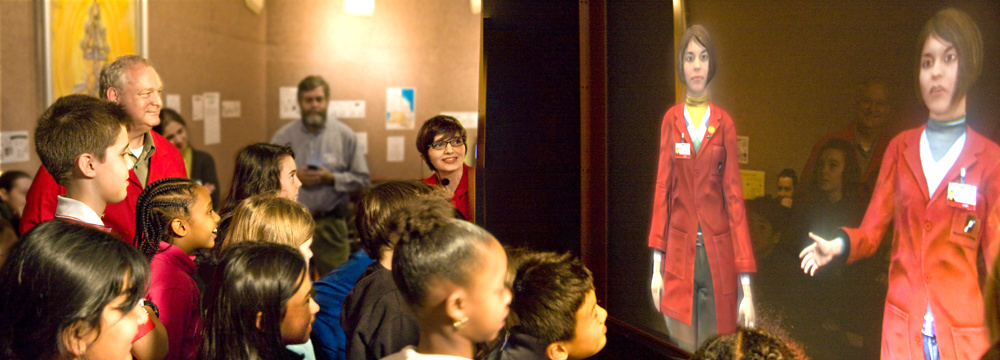
\includegraphics[width=0.9\textwidth,keepaspectratio=true]{images/ada_grace.jpg}
 \caption[Interaksi pemandu museum virtual Ada dan Grace dengan pengunjung di Museum of Science, Boston]{Interaksi pemandu museum virtual Ada dan Grace dengan pengunjung di Museum of Science, Boston \cite{armedwithscience-}.}
 \label{fig:ada_grace}
\vskip .5em
\end{figure}

Secara umum, implementasi ECA belum terlihat di Indonesia. Padahal, ECA dapat dimanfaatkan di berbagai bidang, misalnya di bidang pendidikan dan bidang pariwisata. ECA dapat dimanfaatkan sebagai tutor dalam proses pembelajaran. ECA juga dapat dimanfaatkan untuk membangun kios informasi pariwisata yang kemudian dapat ditempatkan di lokasi-lokasi yang mudah dijangkau oleh wisatawan, seperti di bandara, stasiun, terminal, hotel, atau bahkan di objek pariwisatanya sendiri. Implementasi ECA sebagai pemandu museum seperti Ada dan Grace dapat juga dilakukan di Indonesia untuk menarik lebih banyak orang untuk mengunjungi museum mengingat jumlah rata-rata pengunjung museum-museum di Indonesia pada kurun waktu 2006-2008 hanya mencapai 4,3 juta atau hanya 1,8 persen dari 237 juta lebih penduduk Indonesia (data tahun 2010) \cite{dppobappenas2009, bps2010}.

% RESTU's an Engine for Synthetic Thespian Units

Oleh karena itu, tim PUSPA dan SAMsON dari Program Magister Teknik Elektro, Sekolah Teknik Elektro dan Informatika (STEI), Institut Teknologi Bandung (ITB) bekerjasama dalam mengembangkan \textit{RESTU's an Engine for Synthetic Thespian Units} (RESTU), yang merupakan \textit{engine} untuk membangun ECA. Sebagai sebuah \textit{engine}, RESTU terdiri dari bagian interaksi dan bagian kognisi. Secara umum, bagian interaksi memanfaatkan monitor untuk menampilkan wujud agen, mikrofon sebagai telinga, kamera sebagai mata, dan speaker sebagai mulut. Sedangkan, bagian kognisi dapat dipilih untuk memanfaatkan AIML atau menggunakan \textit{artificial general intelligence} (AGI). Tim PUSPA sendiri memiliki tujuan membangun \textit{PUSPA’s an Understanding Synthespian that Provides Assistance} (PUSPA), yaitu sebuah ECA yang berperan sebagai asisten pribadi. Sedangkan, tim SAMsON memiliki tujuan membangun \textit{Smart Assistant for Museum's Objects Navigation} (SAMsON), yaitu sebuah ECA yang berperan sebagai pemandu museum \cite{nugraha2010}.

\begin{figure}[ht!]
\vskip 1em
\centering
 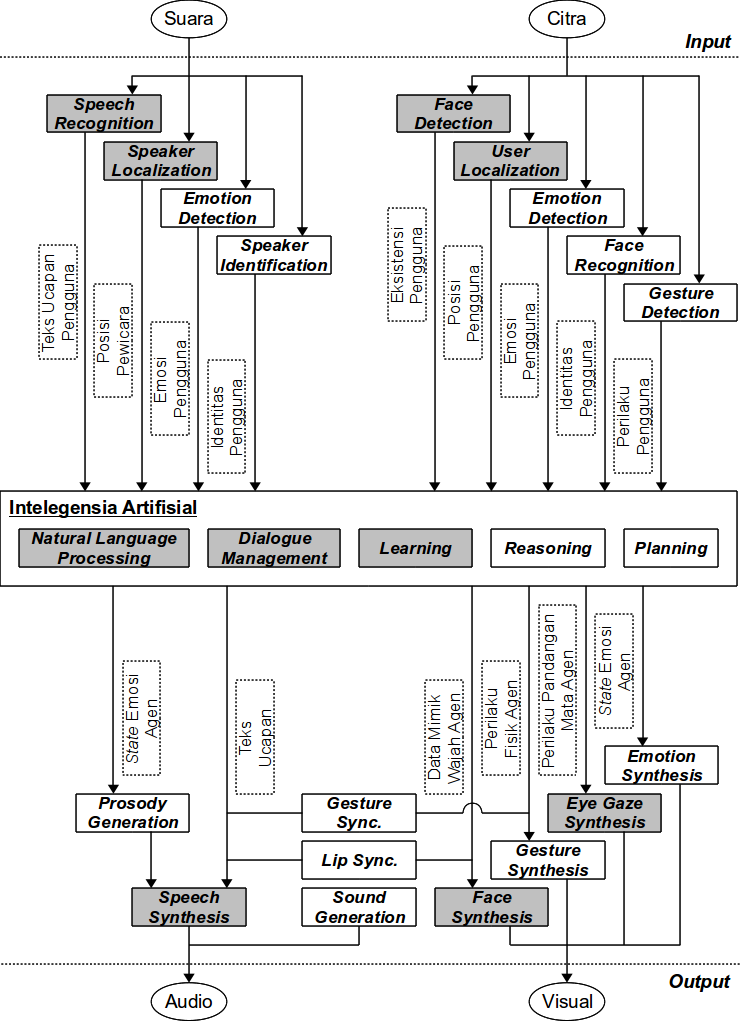
\includegraphics[width=\textwidth,keepaspectratio=true]{images/diagram_blok_eca.png}
 \caption[Diagram blok teknologi penyusun RESTU]{Diagram blok teknologi penyusun RESTU.}
 \label{fig:diagram_blok_eca}
\vskip .5em
\end{figure}

\autoref{fig:diagram_blok_eca} menunjukkan berbagai teknologi terkait ECA yang dapat diimplementasikan pada RESTU. Pada saat ini, teknologi yang diimplementasikan masih terbatas pada teknologi-teknologi yang dalam \autoref{fig:diagram_blok_eca} diberi \textit{background} berwarna abu-abu. Di luar teknologi-teknologi yang sudah tercantum, masih banyak teknologi yang berpotensi meningkatkan kemampuan interaksi ECA. Sebagai contoh, pada pengolahan masukan berupa suara (ucapan), terdapat teknologi \textit{speaker segmentation} dan \textit{speaker tracking}. Implementasi kedua teknologi ini pada RESTU akan memberi kemampuan pada ECA yang dihasilkan untuk mengelola komunikasi dengan pengguna lebih dari satu (\textit{multi-speaker environment}) \cite{martin2001}.

Seperti yang dapat dilihat pada \autoref{fig:diagram_blok_eca}, pada dasarnya komunikasi antara ECA dengan penggunanya hanya memanfaatkan media suara (audio) dan gambar (visual). Meskipun demikian, dari media audiovisual ini, berbagai komunikasi non-verbal dapat berlangsung, misalnya emosi pengguna dapat diketahui dari intonasi suaranya, ekspresi wajahnya, sikap tubuhnya, atau tatapan matanya. Di sisi lain, agen virtual juga dapat menunjukkan emosi yang beragam dengan memberi intonasi tertentu pada suara yang dihasilkan, ekspresi wajah tertentu, sikap tubuh serta pergerakan anggota badan tertentu, atau bahkan dengan tatapan mata tertentu \cite{morency2006, hartmann2005}.


% natural communication: face-to-face, implementation in ECA (need to know speaker location)

Dalam komunikasi tatap muka antar manusia, tatapan mata berperan penting dalam komunikasi non-verbal. Contoh yang paling sederhana adalah tatapan mata dapat memberi petunjuk kepada siapa seseorang sedang berbicara dan dapat memberi petunjuk kondisi emosi seseorang. Oleh karena ECA memiliki wujud, termasuk mata, tatapan mata sebagai salah satu metode komunikasi non-verbal ini juga dapat diimplementasikan untuk menciptakan komunikasi antara manusia dan komputer yang sama alaminya dengan komunikasi antar manusia. Implementasi tatapan mata dan pergerakan mata yang berbeda pada ECA juga telah terbukti memberikan kesan dan tingkat kepuasan yang berbeda bagi penggunanya \cite{lee2002, vanes2002}. Oleh karena itu, sebagai \textit{engine} ECA, RESTU juga harus mengakomodasi fitur ECA yang berupa tatapan dan pergerakan mata agen.

% source localization

Informasi yang dibutuhkan oleh agen dalam menentukan ke arah mana mata agen harus menatap adalah lokasi pengguna atau lawan bicara agen. Dalam RESTU, penentuan lokasi pengguna mungkin dilakukan dengan memanfaatkan informasi yang didapatkan dari: (1) sinyal suara yang ditangkap oleh mikrofon; dan/atau (2) citra yang ditangkap oleh kamera. Mempertimbangkan persyaratan \textit{modularity} dan \textit{extensibility} terkait modalitas masukan dan keluaran yang termasuk dalam persyaratan arsitektur ECA seperti yang tercantum dalam \cite{cassell1998}, penentuan lokasi pengguna dalam RESTU juga harus dapat dilakukan hanya berdasarkan sinyal suara saja atau gambar saja. Meskipun demikian, hasil penentuan lokasi kedua metode tersebut juga dapat dikombinasikan untuk memperoleh lokasi pengguna yang lebih akurat. Penentuan lokasi menggunakan citra yang ditangkap kamera cenderung menghasilkan nilai posisi yang lebih akurat. Akan tetapi, area dimana metode ini dapat digunakan lebih sempit dibandingkan area dimana metode penentuan lokasi menggunakan suara dapat digunakan. Analogi sederhananya adalah telinga manusia dapat mendengar suara yang berasal dari suatu posisi yang terletak di luar jangkauan pandangan mata, misalnya sebuah posisi yang terletak di belakang kepala.

\section{Tujuan Penelitian}

Secara umum, tujuan penelitian ini adalah merancang sebuah subsistem penentuan lokasi pengguna, yang merupakan komponen dari sistem ECA, berdasarkan sinyal suara yang ditangkap oleh mikrofon. Secara lebih khusus, penelitian ini bertujuan: (1) merancang subsistem penentuan lokasi pengguna untuk RESTU dengan memanfaatkan perangkat keras yang murah dan mudah didapatkan, serta perangkat lunak \textit{open source}; (2) mengimplementasikan rancangan yang dihasilkan pada RESTU; serta (3) mengujicoba subsistem penentuan lokasi pengguna yang telah diintegrasikan dalam RESTU.
\section{Batasan Masalah}
\label{sec:batasan}

Dalam perancangan subsistem penentuan lokasi pengguna berdasarkan sinyal suara ini, beberapa asumsi penting yang digunakan adalah sebagai berikut.

\begin{enumerate}
\item Hanya ada satu sumber suara yang dideteksi pada satu waktu.
\item Tidak ada derau dengan intensitas yang tinggi sedemikian sehingga suara ucapan yang tertangkap oleh mikrofon masih terdengar dengan jelas dan dominan.
\item Tidak ada efek akustik dari ruangan, misalnya gema atau gaung. Dengan kata lain, mikrofon hanya menangkap sinyal yang bersifat \textit{direct path} dari sumber suara.
\end{enumerate}

Subsistem penentuan lokasi pengguna yang dirancang memanfaatkan perangkat keras yang murah dan mudah didapatkan, serta perangkat lunak \textit{open source}. Perangkat keras utama yang dibutuhkan oleh subsistem ini adalah komputer, \textit{sound card}, dan mikrofon. Komputer yang digunakan memiliki prosesor Intel$^{\small{\textregistered}}$~Core\texttrademark~2 Duo T8100 2,1 GHz dan memori 2 GB. \textit{Sound card} yang digunakan adalah \textit{USB sound card} tanpa merk yang memiliki dua kanal keluaran (hanya mendukung \textit{sample rate} 48 KHz) dan satu kanal masukan (hanya mendukung \textit{sample rate} 24 KHz). Sedangkan, mikrofon yang digunakan adalah mikrofon \textit{omnidirectional} merk Genius. Subsistem dirancang dan diimplementasikan pada sistem operasi Ubuntu (Linux). Oleh karena kompatibilitas terhadap sistem operasi belum dipertimbangkan, subsistem tidak dapat dipastikan berjalan pada sistem operasi selain Ubuntu (Linux).

Subsistem penentuan lokasi pengguna yang dirancang akan diintegrasikan ke dalam RESTU. Sebagai \textit{showcase}, RESTU akan digunakan untuk membangun sebuah ECA yang berperan sebagai pemandu atau pusat informasi Laboratorium Sistem Komputer dan Kendali (LSKK), ITB. Perangkat keras yang akan digunakan untuk menampilkan pemandu virtual tersebut adalah perangkat \textit{multitouch screen} vertikal milik LSKK yang berdimensi 139 x 60 x 180 centimeter (panjang x lebar x tinggi) seperti yang terlihat pada \autoref{fig:multitouch-foto} dan \autoref{fig:multitouch-dim}. Layar berada di bagian atas dari salah satu sisi terluas perangkat. Pengguna diasumsikan manusia dewasa dengan tinggi badan 150-170 cm yang berdiri di depan layar pada jarak yang wajar diambil saat melakukan komunikasi tatap muka antar manusia (kurang lebih 1 meter). Pengguna juga diasumsikan menghadap ke layar saat berbicara, sedemikian sehingga sinyal suara yang dihasilkan dapat ditangkap oleh mikrofon-mikrofon yang ditempelkan pada perangkat.

\section{Sistematika Pembahasan}

BAB \ref{chap:pendahuluan} menguraikan sejarah singkat dan potensi-potensi pemanfaatan CA, serta proyek pengembangan RESTU, sebuah \textit{engine} ECA, yang kemudian menjadi latar belakang dan motivasi perancangan subsistem penentuan lokasi pengguna berdasarkan sinyal suara. \chaptername~ini juga mendefinisikan batasan-batasan yang digunakan dalam perancangan subsistem tersebut.

BAB \ref{chap:tinjauan_pustaka} membahas landasan teori terkait subsistem penentuan lokasi pengguna berdasarkan sinyal suara yang dirancang dalam penelitian ini. Pembahasan mencakup metode-metode penentuan lokasi sumber suara berdasarkan sinyal suara yang ditangkap.

%\autoref{chap:RESTU} menguraikan arsitektur RESTU secara umum dan menjelaskan bagaimana subsistem yang dirancang diintegrasikan di dalam RESTU.

BAB \ref{chap:perancangan} menjelaskan arsitektur RESTU secara umum dan hubungan subsistem yang dirancang dalam penelitian ini dengan subsistem-subsistem lain yang ada di dalam RESTU, serta menguraikan proses perancangan subsistem penentuan lokasi pengguna berdasarkan sinyal suara, yang meliputi perancangan perangkat keras dan lunak, proses pengambilan dan pengolahan data yang digunakan untuk melatih jaringan syaraf tiruan, serta proses pengujian dan analisis hasil pengujiannya.

BAB \ref{chap:integrasi} membahas proses integrasi subsistem penentuan lokasi pengguna berdasarkan sinyal suara ke dalam RESTU dan proses pengujiannya.

Sedangkan, BAB \ref{chap:kesimpulan} memuat kesimpulan dan saran berdasarkan penelitian yang dilakukan.
\chapter{\uppercase{Tinjauan Pustaka}}
\label{chap:tinjauan_pustaka}

\section{Gelombang Suara Ucapan Manusia}

Gelombang bunyi adalah gelombang longitudinal yang dihasilkan oleh suatu sumber bunyi dan merambat melalui suatu medium. Cepat rambat gelombang bunyi di udara kira-kira $331.5 + 0.6 T_c \, m/s$, dengan $T_c$ adalah temperatur udara dalam satuan Celcius \cite{huang2001}.

Suara ucapan merupakan gelombang bunyi yang dihasilkan oleh pita suara manusia. Dalam menghasilkan ucapan, pita suara dapat bergetar dan menghasilkan gelombang dengan frekuensi yang disebut sebagai frekuensi fundamental ($F_0$) atau \textit{pitch}. Frekuensi fundamental yang dapat dihasilkan oleh pita suara manusia berbeda antara satu orang dengan orang lainnya. Frekuensi fundamental yang umumnya dapat dihasilkan oleh pita suara manusia adalah sebesar 100 Hz pada pria hingga 250 Hz pada wanita dan anak-anak \cite{rabiner2007}. Sumber lain menyebutkan bahwa frekuensi fundamental yang umumnya dapat dihasilkan adalah sebesar 60 Hz pada pria hingga 300 Hz pada wanita dan anak-anak \cite{huang2001}.

Pada umumnya, energi dari sebuah sinyal berada pada frekuensi fundamental hingga harmonik kesepuluhnya. Oleh karena itu, untuk mendapatkan representasi sinyal suara ucapan manusia yang baik, jangkauan frekuensi yang harus dapat ditangkap adalah $F_0$ hingga $10 \, F_0$ \cite{baken1999}. Sebagai contoh, apabila mengacu pada frekuensi fundamental yang dinyatakan dalam \cite{huang2001}, jangkauan frekuensi yang harus dapat ditangkap agar sinyal suara ucapan baik pria, wanita, mau pun anak-anak dapat direpresentasikan dengan baik adalah 60 Hz hingga 3000 Hz. Di bidang telefoni, kanal suara pada jaringan telepon memiliki lebar pita 4000 Hz (frekuensi 0-4000 Hz), meski transmisi suara hanya memanfaatkan frekuensi dalam jangkauan 300-3300 Hz (lebar pita 3000 Hz) \cite{forouzan2003}.

Berdasarkan teorema Nyquist, untuk memastikan suatu sinyal analog yang dikonversi menjadi sinyal digital dapat direproduksi dengan baik, frekuensi \textit{sampling} (\textit{sampling rate}) sekurang-kurangnya dua kali frekuensi tertinggi dari sinyal analog yang di-\textit{sampling} \cite{forouzan2003, baken1999}. Oleh karena itu, apabila diasumsikan bahwa frekuensi tertinggi dari sinyal suara ucapan manusia adalah 4000 Hz, maka frekuensi \textit{sampling} paling rendah yang boleh digunakan adalah sebesar 8000 Hz.

\section{Penentuan Lokasi Sumber Suara}
\label{sec:sound_local}

Manusia dengan indra pendengaran yang berfungsi dengan baik dapat memperkirakan lokasi sumber suara. Ketika seseorang dipanggil oleh rekannya dari belakang, orang tersebut dapat memperkirakan bahwa suara panggilan berasal dari belakang sehingga orang tersebut akan menengok ke arah belakang. Selain itu, seseorang juga dapat memperkirakan arah (sudut) datangnya suara dengan indra pendengaran, yang lokasi sumber suaranya kemudian dapat dikonfirmasi oleh indra penglihatan setelah orang tersebut menengok ke arah perkiraan datangnya suara. Kemampuan menentukan lokasi sumber suara (\textit{sound localization}) yang dimiliki secara alami oleh manusia ini juga akan diimplementasikan pada agen virtual yang dihasilkan oleh RESTU.


\subsection{Penentuan Lokasi Sumber Suara Pada Manusia}
\label{subsec:human_sound_local}

Menurut para peneliti bidang psikoakustik, manusia menggunakan tiga dimensi dalam menentukan lokasi sumber suara \cite{goldstein2010}. Dimensi-dimensi tersebut adalah: (1) \textit{azimuth}, (2) elevasi, dan (3) jarak (\autoref{fig:psychoacoustic-dim}). Untuk menentukan \textit{azimuth}, manusia menggunakan parameter-parameter binaural, yaitu: (1) \textit{interaural time difference} (ITD); (2) \textit{interaural level difference} (ILD), yang dikenal juga sebagai \textit{interaural intensity difference} (IID); dan (3) perubahan spektral (\textit{coloration}) dari bunyi yang mencapai telinga bagian dalam \cite{goldstein2010, gelfand2010, kollmeier2008}. Untuk menentukan elevasi, manusia menggunakan parameter monaural berupa \textit{head-related transfer function} (HRTF). Sedangkan, untuk menentukan jarak, belum ada parameter yang pasti \cite{goldstein2010, gelfand2010}. Pada \autoref{sec:sound_local} ini, pembahasan terkait metode penentuan lokasi sumber suara pada manusia hanya mencakup parameter-parameter binaural, yaitu ITD dan ILD.

\begin{figure}[ht!]
\vskip 1em
\centering
 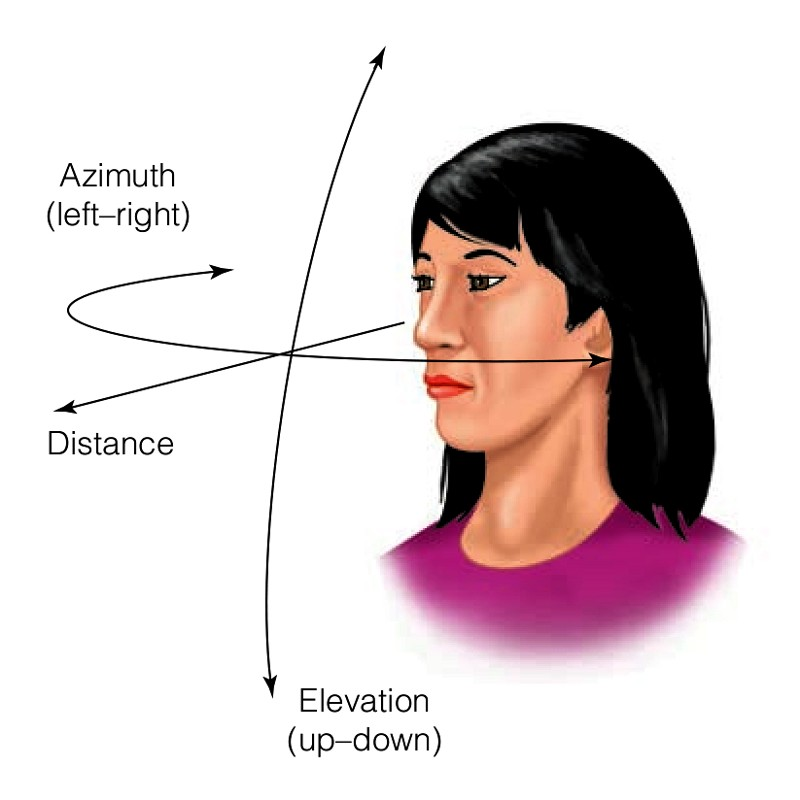
\includegraphics[width=.6\textwidth,keepaspectratio=true]{images/psychoacoustic-dim.jpg}
 \caption[Tiga dimensi yang digunakan manusia untuk menentukan lokasi sumber suara]{Tiga dimensi yang digunakan manusia untuk menentukan lokasi sumber suara \cite{goldstein2010}.}
 \label{fig:psychoacoustic-dim}
\vskip .5em
\end{figure} 

Parameter-parameter binaural didapatkan dengan membandingkan gelombang bunyi yang ditangkap oleh telinga kanan dan kiri. Pada ITD, variabel yang dibandingkan adalah waktu kedatangan gelombang bunyi pada kedua telinga tersebut. Apabila jarak sumber bunyi terhadap kedua telinga sama, misalnya sumber bunyi berada tepat di depan atau di belakang kepala pendengar, parameter ITD bernilai nol (titik A pada \autoref{fig:ilutrasi-itd}). Parameter ITD akan bernilai tidak nol apabila sumber bunyi berada pada \textit{azimuth} tertentu relatif terhadap arah depan kepala. Sebagai contoh, gelombang bunyi yang bersumber pada titik B (\autoref{fig:ilutrasi-itd}) akan diterima oleh telinga kanan terlebih dahulu. Pada gelombang sinusoidal, ITD akan bersifat ambigu antara \textit{leading} atau \textit{lagging} saat perbedaan fasa antara dua gelombang sinyal mencapai $180^o$. Oleh karena itu, ITD rentan menghasilkan nilai yang tidak tepat pada gelombang dengan frekuensi tinggi. 

Pada ILD atau IID, variabel yang dibandingkan adalah \textit{sound pressure level} (SPL) yang diterima oleh telinga kanan dan kiri. Perbedaan SPL yang diterima oleh kedua telinga disebabkan karena kepala membentuk sebuah \textit{acoustic shadow} yang meredam gelombang bunyi yang melaluinya, sehingga intensitas gelombang bunyi yang diterima oleh telinga yang jauh lebih kecil. Meskipun demikian, peredaman ini hanya signifikan pada gelombang dengan frekuensi tinggi (\autoref{fig:ilutrasi-ild-h} dan \autoref{fig:ilutrasi-ild-l}). Oleh karena itu, penentuan \textit{azimuth} lokasi sumber suara pada manusia mengombinasikan ITD dan ILD. ITD untuk gelombang bunyi dengan frekuensi rendah dan ILD untuk gelombang bunyi dengan frekuensi tinggi.

\begin{figure}[ht!]
\vskip 1em
\centering
 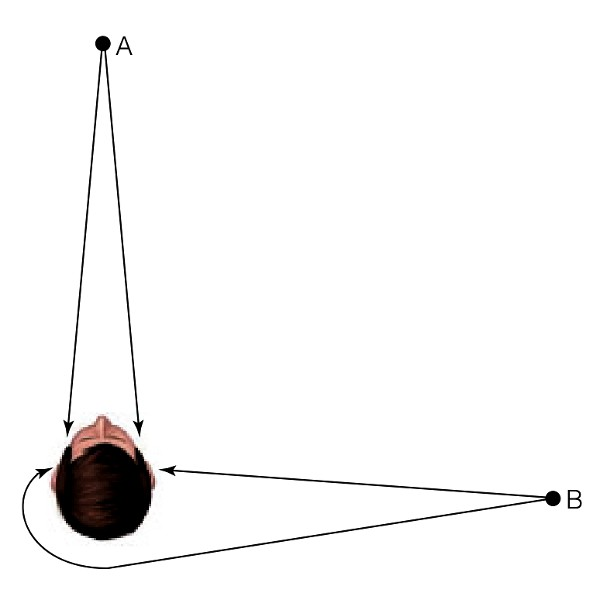
\includegraphics[width=.6\textwidth,keepaspectratio=true]{images/ilustrasi_itd.jpg}
 \caption[Ilustrasi \textit{interaural time difference} (ITD)]{Ilustrasi \textit{interaural time difference} (ITD) \cite{goldstein2010}.}
 \label{fig:ilutrasi-itd}
\vskip .5em
\end{figure}

\begin{figure}[ht!]
\vskip 1em
\centering
 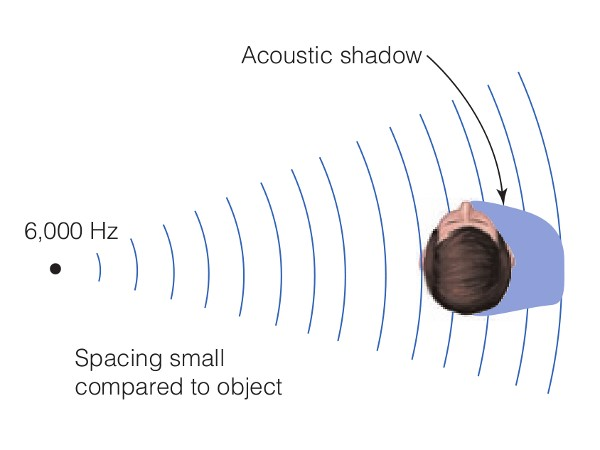
\includegraphics[width=.6\textwidth,keepaspectratio=true]{images/ilustrasi_ild_h.jpg}
 \caption[Ilustrasi \textit{interaural level difference} (ILD) pada gelombang dengan frekuensi tinggi]{Ilustrasi \textit{interaural level difference} (ILD) pada gelombang dengan frekuensi tinggi \cite{goldstein2010}.}
 \label{fig:ilutrasi-ild-h}
\vskip .5em
\end{figure}

\begin{figure}[ht!]
\vskip 1em
\centering
 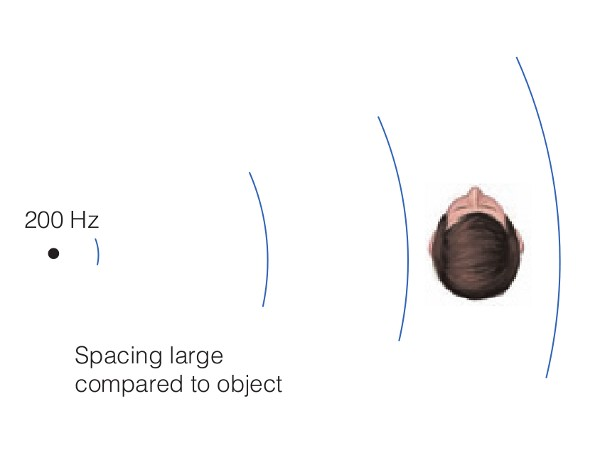
\includegraphics[width=.6\textwidth,keepaspectratio=true]{images/ilustrasi_ild_l.jpg}
 \caption[Ilustrasi \textit{interaural level difference} (ILD) pada gelombang dengan frekuensi rendah]{Ilustrasi \textit{interaural level difference} (ILD) pada gelombang dengan frekuensi rendah \cite{goldstein2010}.}
 \label{fig:ilutrasi-ild-l}
\vskip .5em
\end{figure}

Penentuan lokasi sumber suara yang digunakan RESTU untuk agen virtual (ECA) akan menggunakan konsep yang sama dengan ITD dan ILD, yaitu membandingkan waktu kedatangan dan amplitudo dari gelombang suara ucapan yang tertangkap oleh sepasang mikrofon.


\subsection{\textit{Time Difference of Arrival} (TDOA)}
\label{subsec:tdoa}

Parameter \textit{time difference of arrival} (TDOA) digunakan untuk mengukur perbedaan waktu kedatangan antara suara yang ditangkap oleh mikrofon yang satu dengan mikrofon yang lain dalam sebuah konfigurasi \textit{microphone array}. Pengukuran TDOA dikenal juga sebagai \textit{time delay estimation} (TDE), meskipun sebenarnya TDE sendiri dapat dibagi menjadi pengukuran TDOA dan pengukuran \textit{time of arrival} (TOA) \cite{huang2008}. Pada \autoref{sec:sound_local} ini, pembahasan metode TDE terbatas mengacu pada asumsi-asumsi yang telah didefinisikan pada \autoref{sec:batasan}.

Secara umum, dalam metode TDE terdapat dua model sinyal, yaitu model \textit{free-field} ideal dan model \textit{reverberant} \cite{huang2008, benesty2008}. Dalam \cite{chen2004}, terdapat satu model lagi yang disebut model \textit{multipath}. Tidak seperti model \textit{free-field} ideal yang hanya memperhitungkan sinyal yang bersifat \textit{direct path}, model \textit{multipath} dan model \textit{reverberant} memperhitungkan efek akustik dari ruangan, misalnya pantulan gelombang bunyi (\autoref{fig:propagation_model}). Perbedaan di antara keduanya adalah pada model \textit{multipath} jumlah pantulan dapat diperkirakan, sehingga jumlah \textit{path} gelombang dari sumber bunyi ke mikrofon dapat diketahui dan dapat dihitung. Pada model ini, terdapat variabel $\tau_{lm}$ yang menyatakan waktu tunda relatif antara mikrofon ke-$l$ dengan mikrofon ke-$0$ untuk \textit{path} ke-$m$, dengan $\tau_{01} = 0$. Sedangkan, pada model \textit{reverberant} jumlah \textit{path} sangat banyak sehingga nilai $\tau_{lm}$ sangat sulit untuk dihitung.


\begin{figure}[ht!]
\vskip 1em
\centering
 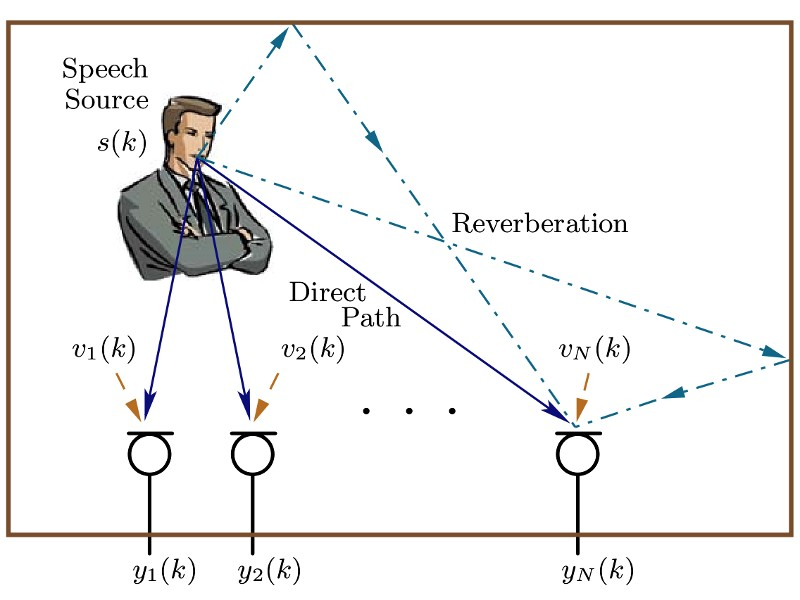
\includegraphics[width=.8\textwidth,keepaspectratio=true]{images/propagation_model.jpg}
 \caption[Ilustrasi model propagasi ideal dan model \textit{reverberant}]{Ilustrasi model propagasi ideal dan model \textit{reverberant} \cite{benesty2008}.}
 \label{fig:propagation_model}
\vskip .5em
\end{figure}


Model \textit{free-field} ideal, juga disebut sebagai model propagasi ideal, mengasumsikan bahwa mikrofon hanya menangkap sinyal yang bersifat \textit{direct path}. Dengan demikian, mikrofon diasumsikan menangkap sinyal yang teredam dan tertunda karena pengaruh propagasi dari sinyal asli yang dihasilkan oleh sumber suara, serta menangkap derau yang bersifat aditif. Mengacu ke skenario yang tergambar pada \autoref{fig:propagation_model}, sinyal yang ditangkap mikrofon $n$ dari sinyal $s$ pada waktu ke-$k$ dapat dinyatakan sebagai \autoref{eq:sinyal_ditangkap}.

\begin{equation}\label{eq:sinyal_ditangkap}
y_{n}(k) = \alpha_{n}s(k - \tau_{n}) + v_{n}(k), \qquad n = 1, 2, \cdots, N
\end{equation}

Pada \autoref{eq:sinyal_ditangkap} tersebut, $\alpha_{n}$ adalah faktor redaman karena propagasi ($0 \leq \alpha_{n} \leq 1$), $\tau_{n}$ adalah waktu yang dibutuhkan untuk propagasi, dan $v_{n}$ adalah derau aditif. Sinyal derau $v_{n}$ diasumsikan tidak berkorelasi dengan sinyal dari sumber suara dan derau yang tertangkap oleh mikrofon yang lain.

TDOA antara mikrofon ke-$i$ dan ke-$j$ dapat didefinisikan sebagai \autoref{eq:tdoa_mic_i_j}.

\begin{equation}\label{eq:tdoa_mic_i_j}
\tau_{ij} \triangleq \tau_{i} - \tau_{j}, \qquad i,j = 1, 2, \cdots, N
\end{equation}

Metode yang paling sederhana dan paling umum digunakan dalam menghitung TDOA adalah \textit{classical cross-correlation} (CCC) \cite{huang2008, benesty2008, chen2004}. Mengacu ke skenario yang tergambar pada \autoref{fig:propagation_model}, CCC antara sinyal $y_{1}(k)$ dan $y_{2}(k)$ dapat didefinisikan sebagai \autoref{eq:CCC_y1k_y2k}.

\begin{equation}\label{eq:CCC_y1k_y2k}
r^{CCC}_{y_{1} y_{2}} (p) = E [y_{1} (k) y_{2} (k + p)]
\end{equation}
 
Kemudian, TDOA dapat diperoleh dari \autoref{eq:tdoa_ccc}.

\begin{equation}\label{eq:tdoa_ccc}
\widehat{\tau}^{CCC}_{y_{1} y_{2}} = \operatorname*{arg\,max}_p r^{CCC}_{y_{1} y_{2}} (p)
\end{equation}

Pada \autoref{eq:CCC_y1k_y2k} dan \autoref{eq:tdoa_ccc}, $p \in [ -\tau_{max} , \tau_{max} ]$ dan $\tau_{max}$ adalah TDOA maksimum yang mungkin terjadi.

CCC sendiri merupakan kasus khusus dari \textit{generalized cross-correlation} (GCC) \cite{huang2008, benesty2008, chen2004}. TDOA pada GCC diperoleh dari \autoref{eq:tdoa_gcc}.

\begin{equation}\label{eq:tdoa_gcc}
\widehat{\tau}^{GCC}_{y_{1} y_{2}} = \operatorname*{arg\,max}_\tau r^{GCC}_{y_{1} y_{2}} (\tau)
\end{equation}

Sedangkan, persamaan GCC didefinisikan sebagai \autoref{eq:gcc_eq}.

\begin{align}\label{eq:gcc_eq}
r^{GCC}_{y_{1} y_{2}} (p) &= F^{-1} [ \Psi_{y_{1} y_{2}} (f) ] \nonumber \\
& = \int_{-\infty}^\infty \Psi_{y_{1} y_{2}} (f) e^{j 2 \pi f p} df \nonumber \\
& = \int_{-\infty}^\infty \vartheta (f) \phi_{y_{1} y_{2}} (f) e^{j 2 \pi f p} df
\end{align}

Pada \autoref{eq:gcc_eq} tersebut, $F^{-1} [ \cdot ]$ menyatakan \textit{inverse discrete-time Fourier transform} (IDTFT), $\Psi_{y_{1} y_{2}} (f)$ adalah \textit{generalized cross-spectrum}, dan $\phi_{y_{1} y_{2}} (f)$ adalah \textit{cross-spectrum}.

\textit{Cross-spectrum} didefinisikan sebagai \autoref{eq:cross_spectrum}, dengan $Y_n (f)$ didefinisikan sebagai \autoref{eq:transform_eq}.

\begin{equation}\label{eq:cross_spectrum}
\phi_{y_{1} y_{2}} (f) = E [ Y_1 (f) Y^*_2 (f) ]
\end{equation}

\begin{equation}\label{eq:transform_eq}
Y_n (f) = \sum_k y_n (k) e^{-j 2 \pi f k}, \qquad n = 1, 2
\end{equation}

Pada \autoref{eq:transform_eq}, $( \cdot )^*$ menyatakan konjugat kompleks.

\textit{Generalized cross-spectrum} didefinisikan sebagai \autoref{eq:gen_cross_spectrum}.

\begin{equation}\label{eq:gen_cross_spectrum}
\Psi_{y_{1} y_{2}} (f) = \vartheta (f) \phi_{y_{1} y_{2}} (f)
\end{equation}

Pada \autoref{eq:gen_cross_spectrum} tersebut, $\vartheta (f)$ adalah fungsi pembobotan pada domain frekuensi. Pada CCC, $\vartheta (f) = 1$.

Persamaan-persamaan GCC di atas dan hubungannya dengan CCC menunjukkan bahwa perhitungan CCC dapat dilakukan menggunakan \textit{discrete Fourier transform} (DFT) dan \textit{inverse} DFT (IDFT), yang dapat diimplementasikan secara efisien memanfaatkan \textit{fast Fourier transform} (FFT).


\subsection{\textit{Peak-to-Peak Amplitude Ratio} (PtPAR)}
\label{subsec:amplitude_ratio}

Parameter \textit{peak-to-peak amplitude ratio} (PtPAR) digunakan untuk mengukur perbedaan amplitudo gelombang antara sinyal suara yang ditangkap oleh mikrofon yang satu dengan mikrofon yang lain.

Intensitas gelombang suara pada sebuah ruang dapat dirumuskan sebagai \autoref{eq:intensitas_suara}.

\begin{equation}\label{eq:intensitas_suara}
I = \frac{P_{av}}{A} = \frac{P_{av}}{4 \pi r^2}
\end{equation}

Pada \autoref{eq:intensitas_suara} tersebut, $P_{av}$ adalah daya rata-rata yang dihasilkan oleh sumber suara, $A$ adalah luas permukaan bola, dan $r$ adalah jari-jari bola \cite{halliday2004}. Dengan demikian, hubungan antara intensitas gelombang suara $I$  dengan sebuah titik yang berjarak $r$ dari sumber suara dapat dinyatakan sebagai \autoref{eq:intensitas_jarak}.

\begin{equation} \label{eq:intensitas_jarak}
I \propto \frac{1}{r^2}
\end{equation}

Sedangkan, daya suatu gelombang dapat dirumuskan sebagai \autoref{eq:daya_gelombang}.

\begin{equation}\label{eq:daya_gelombang}
P = \frac{1}{2}	\mu \omega^2 A^2 v
\end{equation}

Pada \autoref{eq:daya_gelombang} tersebut, $\mu$ adalah rapat massa per satuan panjang medium, $\omega$ adalah frekuensi angular gelombang, $A$ adalah amplitudo gelombang, dan $v$ adalah cepat rambat gelombang \cite{halliday2004}. Dengan demikian, hubungan antara intensitas gelombang suara $I$ dengan amplitudo gelombang suara $A$ dapat dinyatakan sebagai \autoref{eq:intensitas_amplitudo}.

\begin{equation} \label{eq:intensitas_amplitudo}
I \propto {A^2}
\end{equation}

Dari \autoref{eq:intensitas_jarak} dan \autoref{eq:intensitas_amplitudo}, hubungan antara amplitudo gelombang suara $A$ dengan sebuah titik yang berjarak $r$ dari sumber suara dapat dinyatakan sebagai \autoref{eq:amplitudo_jarak}.

\begin{equation} \label{eq:amplitudo_jarak}
A \propto \frac{1}{r}
\end{equation}

Dengan demikian, hubungan perbandingan jarak titik 1 dan 2 dari sumber suara ($r_1$ dan $r_2$) dengan perbandingan amplitudo gelombang yang tertangkap pada kedua titik tersebut ($A_1$ dan $A_2$) dapat dinyatakan sebagai \autoref{eq:amplitudo_jarak_1}.

\begin{equation} \label{eq:amplitudo_jarak_1}
\frac{A_1}{A_2} = \frac{r_2}{r_1}
\end{equation}

Mengacu pada \autoref{eq:amplitudo_jarak} dan skenario yang tergambar pada \autoref{fig:propagation_model}, sinyal yang ditangkap mikrofon $n$ dari sinyal $s$ pada waktu ke-$k$ dengan mengabaikan waktu yang dibutuhkan oleh propagasi gelombang dapat dinyatakan dalam persamaan matematika sebagai \autoref{eq:sinyal_tanpa_propagasi}.

\begin{equation} \label{eq:sinyal_tanpa_propagasi}
y_{n}(k) = \frac{s(k)}{r_n} + v_{n}(k), \qquad n = 1, 2, \cdots, N
\end{equation}

Pada \autoref{eq:sinyal_tanpa_propagasi} tersebut, $r_{n}$ adalah jarak antara mikrofon $n$ dari sumber suara dan $v_{n}$ adalah derau aditif \cite{birchfield2005}.

Berdasarkan eksperimen yang dilakukan dalam \cite{birchfield2005}, dengan menggunakan parameter ILD saja, penentuan lokasi sumber suara dapat dilakukan secara akurat.
%\section{Jaringan Syaraf Tiruan}
%\chapter{\uppercase{Subsistem Penentuan Posisi Pengguna Berdasarkan Sinyal Suara Untuk RESTU}}
\chapter{\uppercase{Perancangan SpeaCal Untuk RESTU}}
\label{chap:perancangan}

%\chapter{\textit{RESTU'S AN ENGINE FOR SYNTHETIC THESPIAN UNITS} (RESTU)}
%\label{chap:RESTU}

\section{\textit{RESTU's an Engine for Synthetic Thespian Units} (RESTU)}
\label{sec:RESTU}

Pengembangan \textit{engine} ECA yang diberi nama \textit{RESTU's an Engine for Synthetic Thespian Units} (RESTU) ini berangkat dari konsep yang terdapat pada \textit{conversational agent}, yaitu gagasan akan mampunya komputer melakukan perbincangan dengan manusia dalam bahasa alami manusia. \textit{Conversational agent}, yang sebelumnya hanya mampu menerima masukan dan memberi keluaran dalam bentuk teks atau suara saja, kemudian berevolusi menjadi \textit{conversational agent} yang memiliki wujud, misalnya berupa karakter manusia dalam bentuk 3-dimensi (3D), yang dikenal sebagai \textit{embodied conversational agent} (ECA) atau \textit{embodied conversational interface agent}. Wujud yang dimiliki oleh agen memungkinkan lebih banyak cara yang dapat digunakan dalam komunikasi antara manusia dan komputer, misalnya arah tatapan mata, gerakan badan, dan mimik muka. Dengan kata lain, agen memiliki kemampuan untuk melakukan komunikasi non-verbal dengan pengguna, seperti yang dilakukan dalam komunikasi tatap muka antar manusia, sehingga berpotensi menciptakan komunikasi yang lebih alami dan pengalaman interaksi yang lebih kaya bagi pengguna.

Fitur dasar dari ECA yang dibangun dengan \textit{engine} ini adalah mampu melakukan perbincangan dengan penggunanya dalam Bahasa Indonesia. Fitur dasar produk ECA yang lain akan sangat bergantung pada peran agen virtual. Sebagai contoh, apabila produk ECA ditujukan untuk berperan sebagai asisten, agen virtual akan mampu memahami permintaan penggunanya dan berusaha mewujudkannya. Apabila produk ECA ditujukan untuk berperan sebagai pemandu museum, agen virtual akan mampu memahami pertanyaan pengguna dan berusaha untuk menjawab serta menjelaskannya. Meskipun demikian, perlu diingat bahwa tindakan-tindakan tersebut sangat bergantung pada pengetahuan yang dimiliki oleh agen virtual. Sebagai contoh, agen virtual yang berperan sebagai pemandu museum hanya dapat menjawab pertanyaan-pertanyaan terkait museum. Fitur yang lain adalah agen virtual diwujudkan dalam tampilan 3D yang dilengkapi dengan kemampuan menggerakkan anggota badannya. Selain dapat menggerakkan bibir saat berbicara, agen virtual dapat menengokkan kepalanya untuk memandang lawan bicaranya. Agen juga dapat menunjukkan pose tertentu untuk mencapai tujuannya, misalnya menunjukkan suatu gambar ke pengguna, atau sekedar untuk membangun suasana percakapan yang tidak kaku.

\begin{figure}[ht!]
\vskip 1em
\centering
 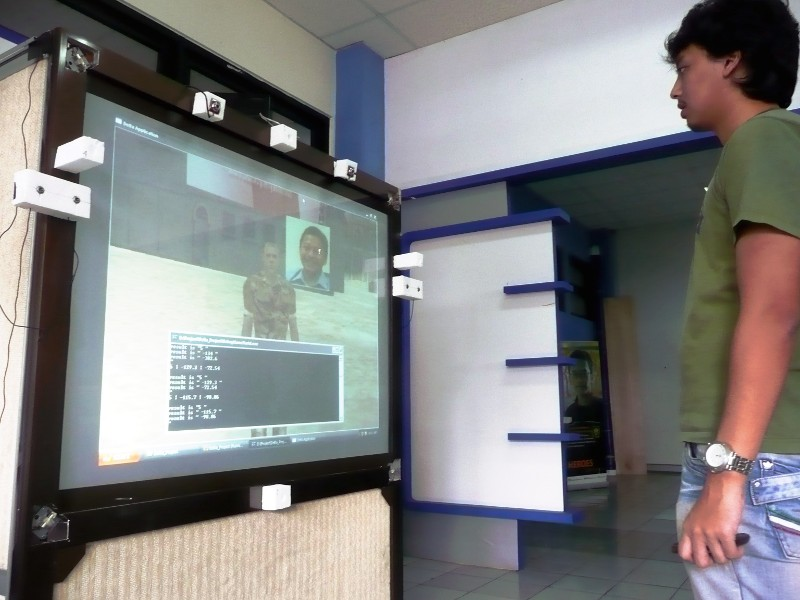
\includegraphics[width=0.9\textwidth,keepaspectratio=true]{images/prototipe_lskk.jpg}
 \caption[Interaksi pengguna dengan prototipe pemandu virtual LSKK yang dibangun dengan RESTU]{Interaksi pengguna dengan prototipe pemandu virtual LSKK yang dibangun dengan RESTU.}
 \label{fig:prototipe_lskk}
\vskip .5em
\end{figure}

Secara umum, RESTU disusun oleh teknologi pemrosesan bahasa alami, pemrosesan suara, pemrosesan citra, grafis 3D, dan kecerdasan artifisial. Teknologi pemrosesan bahasa alami, mencakup teknologi pengenalan suara dan sintesis suara. Teknologi pemrosesan suara digunakan dalam fungsi penentuan lokasi pengguna berdasarkan suara dan teknologi pemrosesan citra digunakan dalam fungsi pengenalan wajah untuk menentukan lokasi pengguna berdasarkan citra. Teknologi grafis digunakan untuk mewujudkan karakter virtual, perilakunya, dan lingkungannya. Sedangkan, teknologi kecerdasan artifisial dimanfaatkan untuk menyusun respons terhadap masukan dari pengguna yang diterima oleh agen berdasarkan pengetahuan yang dimilikinya.

Fungsi-fungsi yang menyusun RESTU tersebut dapat dikelompokkan menjadi dua bagian, yaitu bagian kognitif dan bagian interaksi. Fungsi kecerdasan artifisial menyusun bagian kognitif. Sedangkan, bagian interaksi tersusun dari fungsi pengenalan suara, sintesis suara, penentuan lokasi pengguna baik menggunakan suara mau pun citra, dan antarmuka grafis. Dengan mengikuti pengelompokan tersebut, di sisi implementasi RESTU dibangun dengan menggunakan dua kelompok \textit{server}, yaitu \textit{Artificial Intelligence (AI) Engine Server} dan \textit{User Interface (UI) Engine Server}. UI Engine Server dapat dibagi menjadi \textit{Camera Engine Server}, \textit{Speech Engine Server}, dan \textit{Graphical User Interface (GUI) Engine Server}. Diagram aliran data antar \textit{server}, atau modul yang ada di dalamnya, ditunjukkan oleh \autoref{fig:RESTU_arch}.

\begin{figure}[ht!]
\vskip 1em
\centering
 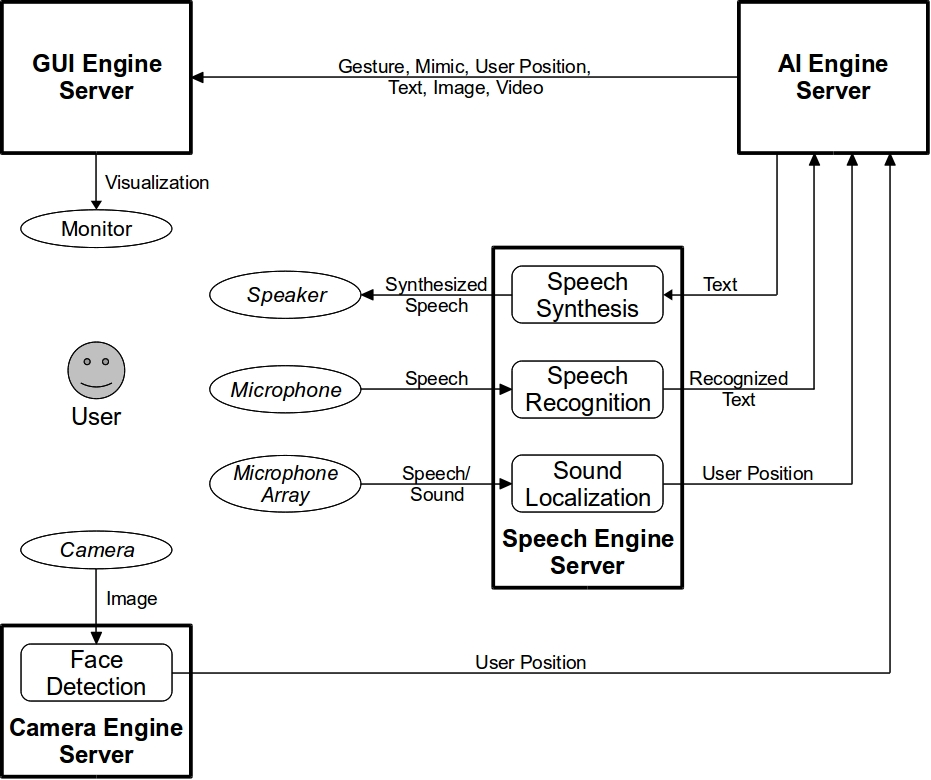
\includegraphics[width=.95\textwidth,keepaspectratio=true]{images/RESTU_arch.jpg}
 \caption[Diagram aliran data RESTU]{Diagram aliran data RESTU.}
 \label{fig:RESTU_arch}
\vskip .5em
\end{figure}


\section{\textit{Speaker Localization} (SpeaCal)}
\label{sec:speacal}

SpeaCal, yang berasal dari istilah \textit{Speaker Localization}, merupakan subsistem penentuan posisi pengguna berdasarkan sinyal suara, yang dalam \autoref{fig:RESTU_arch} disebut sebagai \textit{Sound Localization}. \autoref{sec:speacal} ini akan menguraikan proses perancangan SpeaCal yang menggunakan model perancangan iteratif. Perancangan melalui tahap pendefinisian kebutuhan, penentuan spesifikasi, pembuatan desain, pengimplementasian desain, serta pengujian dan evaluasi. Proses iterasi dilakukan pada tiga tahap yang disebutkan terakhir.

Tahap pembuatan desain meliputi pembuatan desain perangkat lunak dan desain perangkat keras, yang kemudian akan diimplementasikan pada tahap implementasi. Sedangkan, tahap pengujian dan evaluasi meliputi pengambilan data latih dan data uji yang akan digunakan untuk melatih dan menguji JST. Analisis kemudian dilakukan terhadap semua data yang diperoleh, tanpa membedakan antara data latih dan data uji, untuk menentukan apakah desain perangkat lunak dan perangkat keras dapat menghasilkan data yang cukup konsisten sehingga dapat digunakan untuk melatih JST. Apabila data tidak cukup konsisten, proses perancangan akan kembali pada tahap pembuatan desain.

\subsection{Definisi Kebutuhan}

SpeaCal dikembangkan spesifik untuk RESTU. Dari \autoref{chap:pendahuluan} dan \autoref{sec:RESTU}, fungsi penentuan posisi pengguna dibutuhkan untuk mengetahui ke arah mana mata atau kepala agen virtual harus menatap atau menoleh. Dalam komunikasi tatap muka antar manusia, kontak mata diperlukan untuk menunjukkan perhatian terhadap lawan bicara dan topik pembicaraan. meskipun demikian, kontak mata tidak berarti mata seseorang \textit{selalu} menatap lawan bicara \textit{tepat} di matanya selama percakapan.

Dengan demikian, SpeaCal harus dapat menghasilkan informasi \textit{perkiraan} posisi pengguna berdasarkan suara pengguna yang ditangkap oleh mikrofon. Informasi perkiraan posisi yang menjadi prioritas utama adalah informasi \textit{azimuth}. Informasi ini kemudian harus dapat digunakan oleh \textit{AI Engine}, atau \textit{GUI Engine} secara langsung, untuk menentukan ke arah mana mata atau kepala agen virtual harus menatap atau menoleh.

Definisi kebutuhan di atas dapat digambarkan oleh \autoref{fig:speacal_block_diagram}.

\begin{figure}[ht!]
\vskip 1em
\centering
 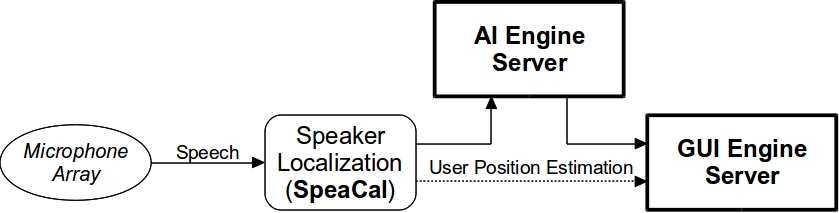
\includegraphics[width=.9\textwidth,keepaspectratio=true]{images/speacal_block_diagram.jpg}
 \caption[Ilustrasi definisi kebutuhan SpeaCal]{Ilustrasi definisi kebutuhan SpeaCal.}
 \label{fig:speacal_block_diagram}
\vskip .5em
\end{figure}

%%%%%%%%%%%%%%%%%%%%%%%%%%%%%%%%%%%%%%%%%%%%%%%%%%5

\subsection{Spesifikasi}
\label{subsec:spesifikasi}

Dari definisi kebutuhan di atas, SpeaCal harus mampu memperkirakan posisi pengguna berdasarkan suara pengguna yang ditangkap oleh mikrofon. Untuk melakukannya, SpeaCal akan menggunakan parameter ITD dan/atau ILD yang membandingkan dua sinyal. Oleh karena itu, diperlukan lebih dari satu mikrofon untuk menangkap suara pengguna. Pada manusia, dua indera pendengaran dapat digunakan untuk memperkirakan \textit{azimuth} posisi sumber suara. Mengacu pada fakta ini, SpeaCal akan menggunakan empat buah mikrofon yang dipasang di bagian atas, bawah, kanan, dan kiri perangkat. Dengan mikrofon-mikrofon tersebut (selanjutnya disebut \textit{microphone array}) diharapkan informasi posisi sumber suara yang diperoleh tidak hanya \textit{azimuth}, tetapi juga \textit{elevation}.

Untuk menangkap sinyal dari mikrofon dibutuhkan \textit{sound card}. Sinyal suara yang akan ditangkap oleh mikrofon adalah suara manusia, sehingga satu kanal suara (mono) saja cukup untuk merepresentasikan sinyal yang ditangkap dengan baik. Dengan demikian, untuk menangkap sinyal dari empat mikrofon dibutuhkan empat kanal suara. Dari hasil survei, \textit{sound card} yang dapat diakses (dibeli) dengan mudah dan harganya murah adalah \textit{USB sound card}. Perangkat seharga Rp 28.000,00 ini memiliki satu kanal masukan yang dapat dimanfaatkan untuk menerima sinyal dari mikrofon.

Untuk mengelola empat \textit{sound card} ini dibutuhkan sebuah program (pustaka) yang mampu mengakses \textit{buffer} yang dimiliki \textit{sound card}, sehingga data sinyal yang tertangkap oleh mikrofon dapat disimpan dalam sebuah file. File-file representasi sinyal dari setiap mikrofon kemudian akan diolah untuk menghitung TDOA, sebagai parameter ITD, dan PtPAR, sebagai parameter ILD. Perhitungan TDOA akan menggunakan DFT agar komputasi dapat dilakukan dengan lebih cepat. Oleh karena itu, dibutuhkan pustaka yang mampu melakukan FFT.

Parameter TDOA dan/atau PtPAR inilah yang kemudian digunakan oleh JST untuk memperkirakan posisi pengguna. Untuk membangun sebuah JST diperlukan kumpulan data latih dan data uji yang memuat nilai masukan, berupa nilai TDOA dan/atau PtPAR, dan nilai keluaran, berupa posisi. Data latih digunakan untuk membangun (melatih) JST, sedangkan data uji digunakan untuk menguji jaringan yang telah dilatih. JST tersebut kemudian digunakan untuk proses penentuan posisi pengguna saat SpeaCal telah diintegrasikan dalam RESTU. Oleh karena itu, dibutuhkan pustaka pustaka yang mampu membangun dan menggunakan JST.

Dengan demikian, SpeaCal harus mampu:

\begin{enumerate}
\item menangkap suara pengguna dengan menggunakan \textit{microphone array}, yang terdiri dari empat mikrofon, secara bersamaan;
\item menghitung TDOA dari sinyal suara yang ditangkap oleh \textit{microphone array};
\item menghitung PtPAR dari sinyal suara yang ditangkap oleh \textit{microphone array};
\item menyimpan data TDOA, PtPAR, dan posisi untuk membuat data latih dan data uji JST;
\item melatih JST dengan nilai TDOA dan PtPAR yang didapatkan selama pengambilan data latih;
\item menguji JST dengan nilai TDOA dan PtPAR yang didapatkan selama pengambilan data uji;
\item menggunakan JST untuk menghasilkan informasi perkiraan posisi pengguna (sumber suara); dan
\item mengirimkan informasi perkiraan posisi pengguna ke subsistem lain (\textit{AI Engine} atau \textit{GUI Engine}).
\end{enumerate}

Perangkat keras yang akan digunakan meliputi:

\begin{itemize}
\item perangkat \textit{multitouch screen} vertikal milik LSKK yang berdimensi 139 x 60 x 180 centimeter (panjang x lebar x tinggi) (\autoref{fig:multitouch-foto}, \autoref{fig:multitouch-dim});

\item komputer:
\begin{itemize}
\item untuk perancangan serta pengambilan data latih dan uji: laptop Dell XPS M1330 dengan prosesor Intel$^{\small{\textregistered}}$~Core\texttrademark~2 Duo T8100 2,1 GHz dan memori 2 GB, dan
\item untuk demo: komputer rakitan dengan prosesor Intel$^{\small{\textregistered}}$~Core\texttrademark~i7 2,67 GHz dan memori 2 GB;
\end{itemize}

\item \textit{USB sound card} tanpa merk (4 buah), dengan dua kanal keluaran yang hanya mendukung \textit{sample rate} 48 KHz dan satu kanal masukan yang hanya mendukung \textit{sample rate} 24 KHz (\autoref{fig:foto_sound_card_dan_hub});

\item \textit{USB hub} merk Belkin, yang memiliki empat \textit{port} (\autoref{fig:foto_sound_card_dan_hub}); 

\item mikrofon (4 buah) merk Genius seri MIC-01A, yang bagian tangkainya dipotong dan bagian kepalanya ditancapkan pada \textit{styrofoam} yang ditempelkan pada perangkat \textit{multitouch screen} vertikal (\autoref{fig:foto_mic_styrofoam}); dan

\item \textit{speaker} merk Genius seri SP-i150;
\end{itemize}

Sedangkan, perangkat lunak yang akan digunakan meliputi:

\begin{itemize}
\item sistem operasi: Ubuntu 10.04.2 LTS;
\item bahasa pemrograman: C, C++;
\item IDE: CodeBlocks;
\item pustaka: C Std Lib, C POSIX Lib, C++ Std Lib, Portaudio, FFTW3, FANN, Boost, wxWidgets;
\item pengolah data: gedit, OpenOffice Calc;
\item pendukung: Audacity, Octave.
\end{itemize}

\begin{figure}[ht!]
\vskip 1em
\centering
 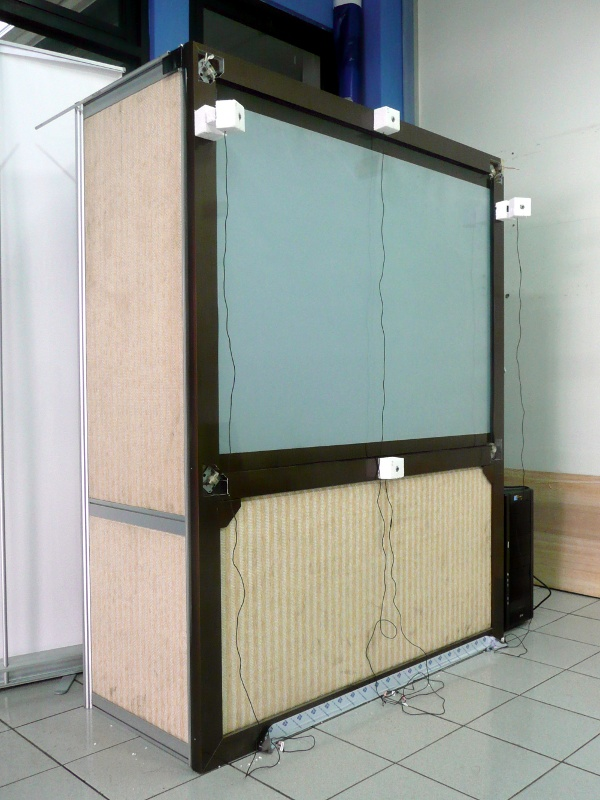
\includegraphics[height=12cm,keepaspectratio=true]{images/multitouch.jpg}
 \caption[Foto perangkat \textit{multitouch screen} vertikal yang akan digunakan untuk demo RESTU]{Foto perangkat \textit{multitouch screen} vertikal yang akan digunakan untuk demo RESTU.}
 \label{fig:multitouch-foto}
\vskip .5em
\end{figure}

\begin{figure}[htp!]
\vskip 1em
\centering
 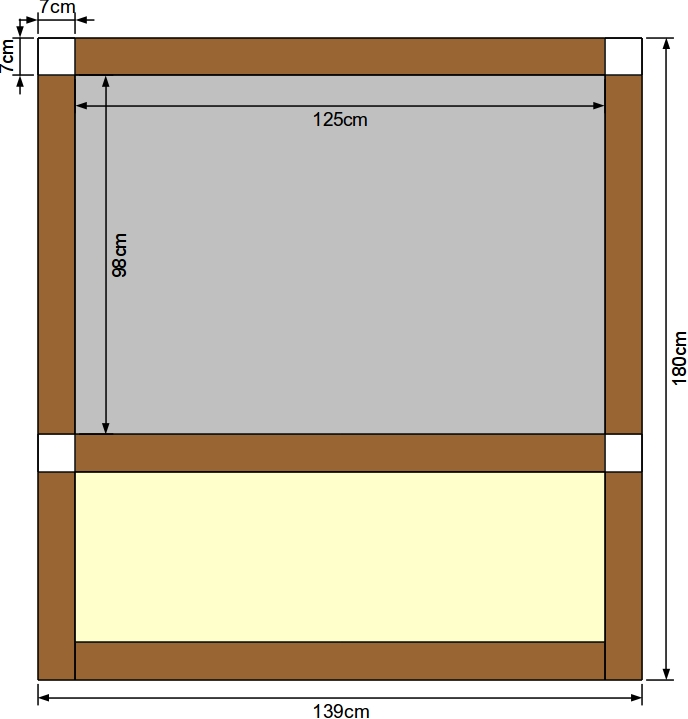
\includegraphics[height=12cm,keepaspectratio=true]{images/multitouch-dim.jpg}
 \caption[Dimensi bagian muka perangkat \textit{multitouch screen} vertikal yang akan digunakan untuk demo RESTU]{Dimensi bagian muka perangkat \textit{multitouch screen} vertikal yang akan digunakan untuk demo RESTU.}
 \label{fig:multitouch-dim}
\vskip .5em
\end{figure}

\begin{figure}[htp!]
\vskip 1em
  \begin{center}
    \subfigure[Foto \textit{USB sound card} dan \textit{USB hub}.]
    {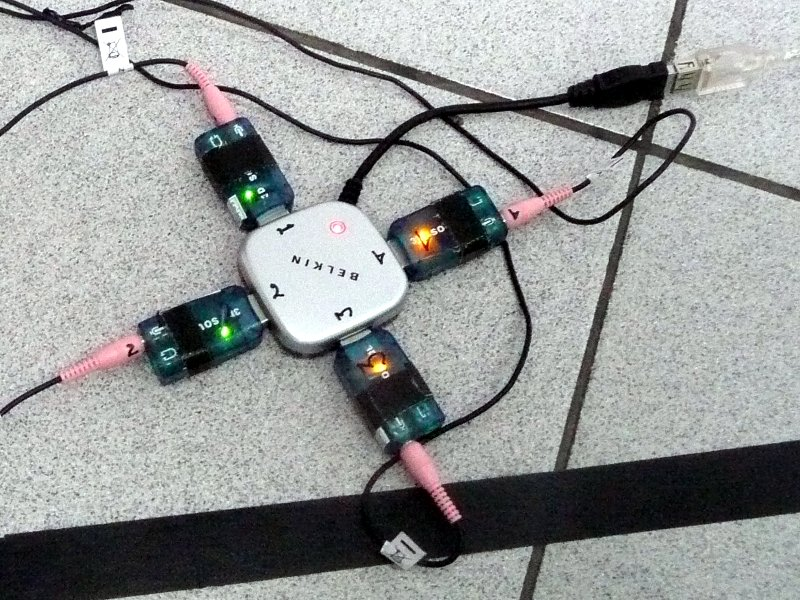
\includegraphics[width=.475\textwidth,keepaspectratio=true]{images/foto_sound_card_dan_hub.jpg}
    \label{fig:foto_sound_card_dan_hub}}
    \subfigure[Foto instalasi mikrofon pada perangkat \textit{multitouch screen} vertikal.]
    {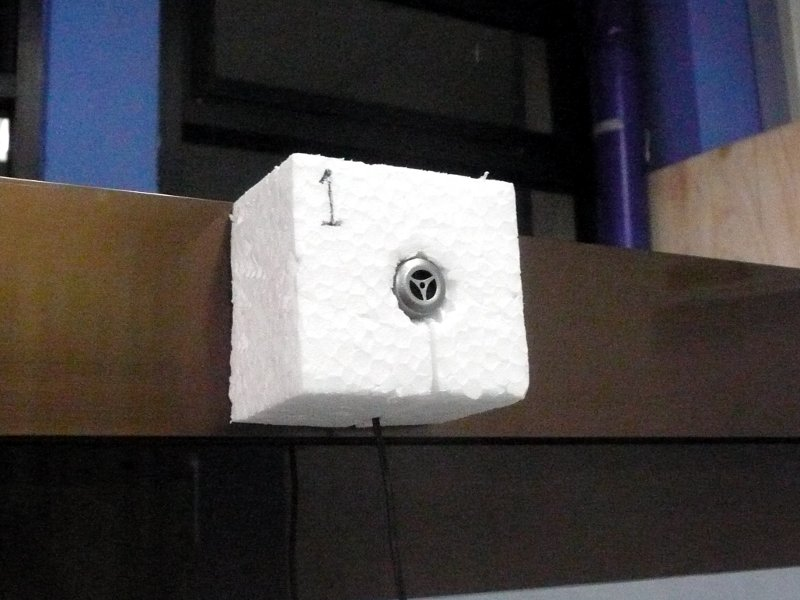
\includegraphics[width=.475\textwidth,keepaspectratio=true]{images/foto_mic_styrofoam.jpg}
    \label{fig:foto_mic_styrofoam}}
  \end{center}
  \caption[Foto \textit{USB sound card}, \textit{USB hub}, dan mikrofon yang digunakan dalam perancangan]{Foto sebagian perangkat keras yang digunakan dalam perancangan.}
  \vskip .5em
\end{figure}


\subsection{Iterasi I: Desain}
\label{subsec:iter1_desain}

\subsubsection{Perangkat Lunak}

Dari \autoref{subsec:spesifikasi} dapat didefinisikan tiga perangkat lunak (program) utama yang dibutuhkan dalam perancangan subsistem penentuan posisi pengguna berdasarkan sinyal suara, yaitu:
\begin{enumerate}
\item SpeaCalTrain, yaitu perangkat lunak (program) yang digunakan untuk memperoleh data latih dan data uji untuk JST;
\item SpeaCal, yaitu perangkat lunak (program) yang digunakan untuk memperkirakan posisi pengguna memanfaatkan JST; dan
\item perangkat lunak (program) pendukung yang digunakan untuk melatih JST dengan memanfaatkan data latih dan mengujinya dengan memanfaatkan data uji.
\end{enumerate}

Dalam \autoref{subsec:spesifikasi} telah dijelaskan bahwa penentuan posisi pengguna akan memanfaatkan parameter TDOA dan PtPAR. Kedua parameter tersebut akan dihitung dari empat sinyal suara yang ditangkap oleh empat mikrofon. Oleh karena itu, fungsi penangkap sinyal suara serta fungsi penghitung parameter TDOA dan PtPAR menjadi inti dari SpeaCalTrain dan SpeaCal. 

\autoref{fig:flowchart_main_wxspeacaltrain} menunjukkan alur program yang digunakan untuk mendapatkan data latih dan data uji untuk JST. \autoref{fig:flowchart_main_wxspeacal} menunjukkan alur program yang digunakan untuk memperkirakan posisi pengguna memanfaatkan JST. Sedangkan, \autoref{fig:flowchart_main_anntraining} menunjukkan alur program yang digunakan untuk melatih JST.

\autoref{fig:flowchart_record_wxspeacaltrain} dan \autoref{fig:flowchart_record_wxspeacal} menunjukkan alur fungsi penangkap sinyal pada SpeaCalTrain dan SpeaCal. Sedangkan, \autoref{fig:flowchart_compute_wxspeacaltrain} dan \autoref{fig:flowchart_compute_wxspeacal} menunjukkan alur fungsi penghitung parameter TDOA dan PtPAR. Pada prinsipnya, fungsi penangkap sinyal suara dan penghitung parameter yang digunakan pada kedua program adalah sama. Perbedaannya terletak pada adanya proses menyimpan data pada program SpeaCalTrain dan adanya proses menjalankan JST pada program SpeaCal.

Durasi sampel sinyal suara yang direkam oleh fungsi penangkap sinyal dapat diatur secara fleksibel. Akan tetapi, perlu diingat bahwa durasi sampel sinyal suara berpengaruh pada banyaknya \textit{frame} yang harus diolah oleh fungsi penghitung parameter. Dari pengamatan, durasi sampel berbanding lurus dengan waktu yang dibutuhkan oleh fungsi penghitung parameter untuk menyelesaikan operasinya. Oleh karena itu, apabila durasi sampel sinyal diset $x$ detik, fungsi penangkap sinyal harus diset ke \textit{idle} selama $x$ detik setiap kali selesai merekam sinyal selama $x$ detik untuk memastikan bahwa fungsi penghitung parameter telah menyelesaikan operasinya. Dalam perancangan ini, durasi yang digunakan adalah 0,5 dan 1 detik, sehingga nilai perkiraan posisi pengguna diperbarui setiap 1 dan 2 detik.

Data yang disimpan pada program SpeaCalTrain terdiri dari data suara dalam file berekstensi \texttt{raw} dan data TDOA serta PtPAR yang tertulis dalam sebuah file teks. Format penulisan file teks yang memuat data TDOA dan PtPAR disesuaikan dengan format data latih JST. Contoh penulisan file teks data tersebut dapat dilihat pada \autoref{lst:teks_data}. Baris pertama dalam file menunjukkan jumlah data (pasangan masukan dan keluaran) yang tercantum dalam file tersebut, jumlah masukan, dan jumlah keluaran. Dalam contoh yang tercantum pada \autoref{lst:teks_data}, jumlah data adalah 120, jumlah masukan 12, dan jumlah keluaran 3. Baris-baris selanjutnya terbagi atas dua macam, yaitu baris genap menuliskan data masukan dan baris ganjil menuliskan data keluaran yang bersesuaian. Dalam contoh yang tercantum pada \autoref{lst:teks_data}, baris data masukan mencantumkan enam data TDOA yang disusul dengan enam data PtPAR dan baris data keluaran mencantumkan representasi sebuah titik dalam koordinat Cartesian.

\singlespacing
\begin{figure}[htp!]
\vskip 1em
\begin{lstlisting}
120	12	3
1.375	2.833	3.208	1.417	1.792	0.417	-7.214	-11.371	-15.296	-4.156	-8.081	-3.925
190	30	60
-1.458	2.500	1.292	3.833	2.667	-1.125	-7.244	-11.366	-15.586	-4.121	-8.341	-4.220
190	30	60
0.000	7.292	2.667	2.917	2.667	-0.250	-7.097	-11.227	-15.222	-4.130	-8.125	-3.995
190	30	60
...
\end{lstlisting}
\caption[Contoh penulisan data TDOA dan PtPAR dalam file teks data]{Contoh penulisan data TDOA dan PtPAR dalam file teks data.}
\label{lst:teks_data}
\vskip .5em
\end{figure}
\onehalfspacing

\begin{figure}[htp!]
\vskip 1em
\centering
 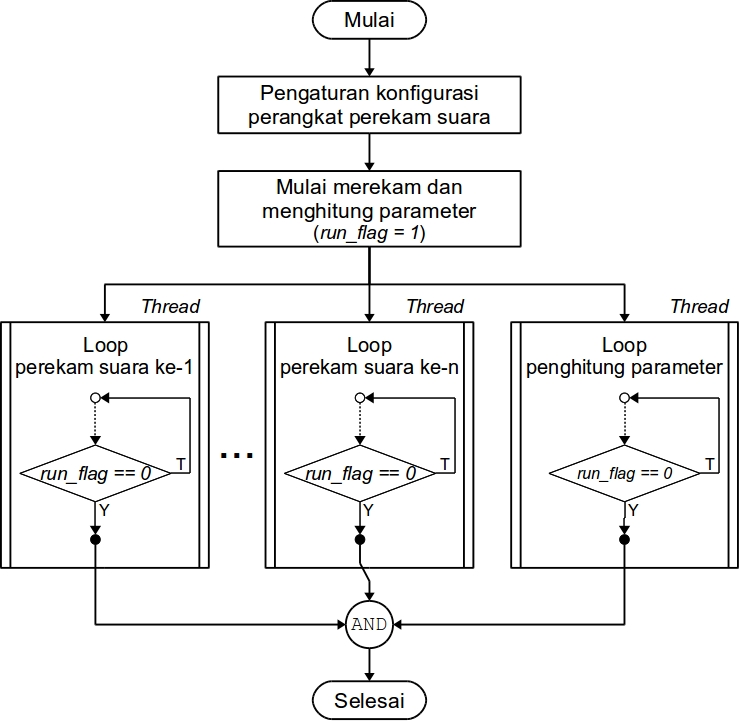
\includegraphics[scale=.5,keepaspectratio=true]{images/flowchart_main_wxspeacaltrain.jpg}
 \caption[Diagram alir SpeaCalTrain]{Diagram alir SpeaCalTrain.}
 \label{fig:flowchart_main_wxspeacaltrain}
\vskip .5em
\end{figure}

\begin{figure}[htp!]
\vskip 1em
\centering
 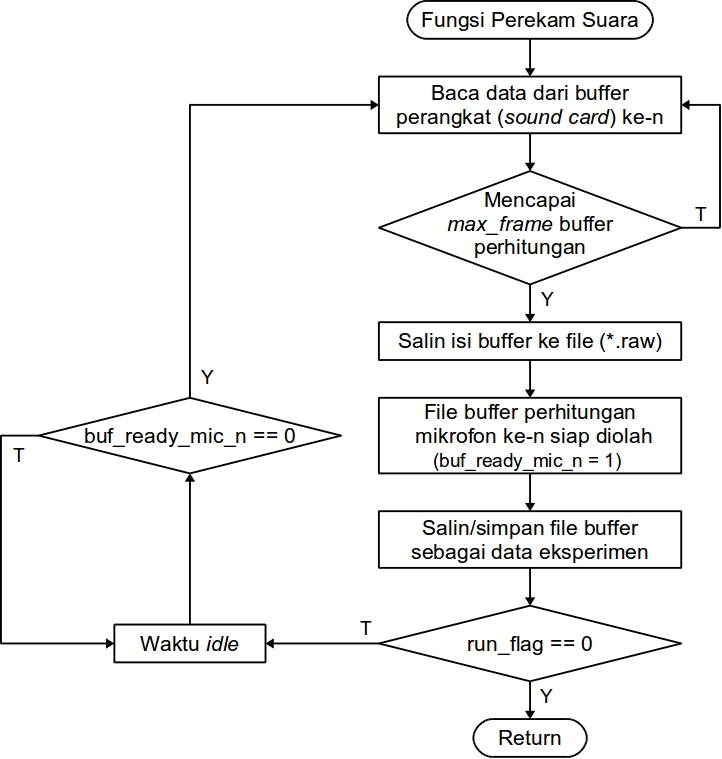
\includegraphics[scale=.5,keepaspectratio=true]{images/flowchart_record_wxspeacaltrain.jpg}
 \caption[Diagram alir fungsi perekam suara pada SpeaCalTrain]{Diagram alir fungsi perekam suara pada SpeaCalTrain.}
 \label{fig:flowchart_record_wxspeacaltrain}
\vskip .5em
\end{figure}

\begin{figure}[htp!]
\vskip 1em
\centering
 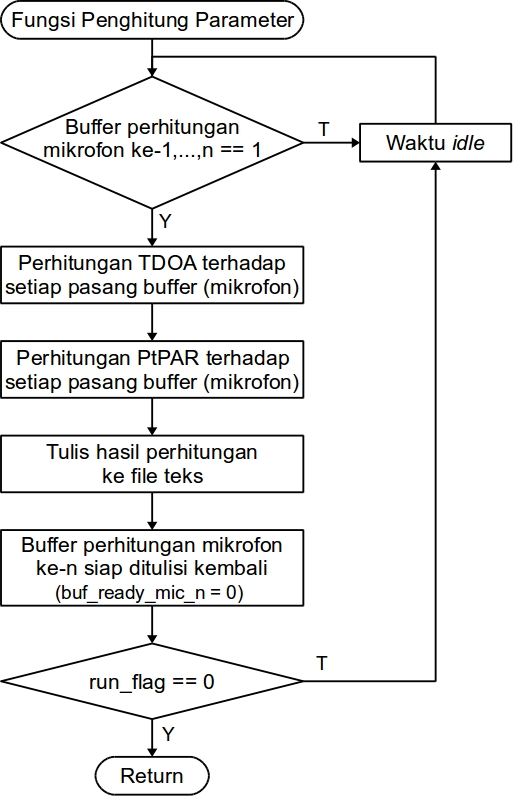
\includegraphics[scale=.5,keepaspectratio=true]{images/flowchart_compute_wxspeacaltrain.jpg}
 \caption[Diagram alir fungsi penghitung parameter TDOA dan PtPAR pada SpeaCalTrain]{Diagram alir fungsi penghitung parameter TDOA dan PtPAR pada SpeaCalTrain.}
 \label{fig:flowchart_compute_wxspeacaltrain}
\vskip .5em
\end{figure}

\begin{figure}[htp!]
\vskip 1em
\centering
 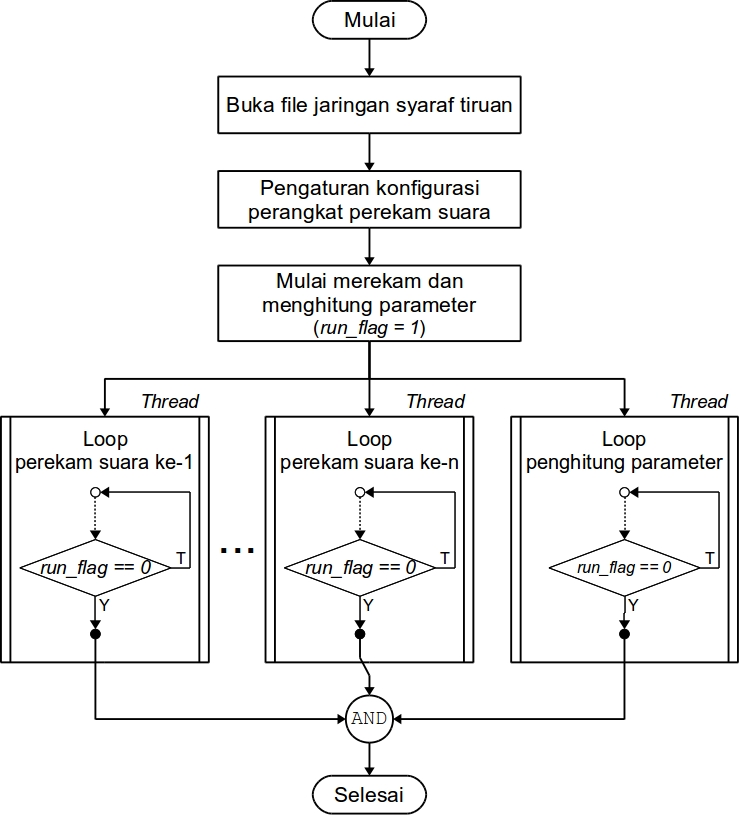
\includegraphics[scale=.5,keepaspectratio=true]{images/flowchart_main_wxspeacal.jpg}
 \caption[Diagram alir SpeaCal]{Diagram alir SpeaCal.}
 \label{fig:flowchart_main_wxspeacal}
\vskip .5em
\end{figure}

\begin{figure}[htp!]
\vskip 1em
\centering
 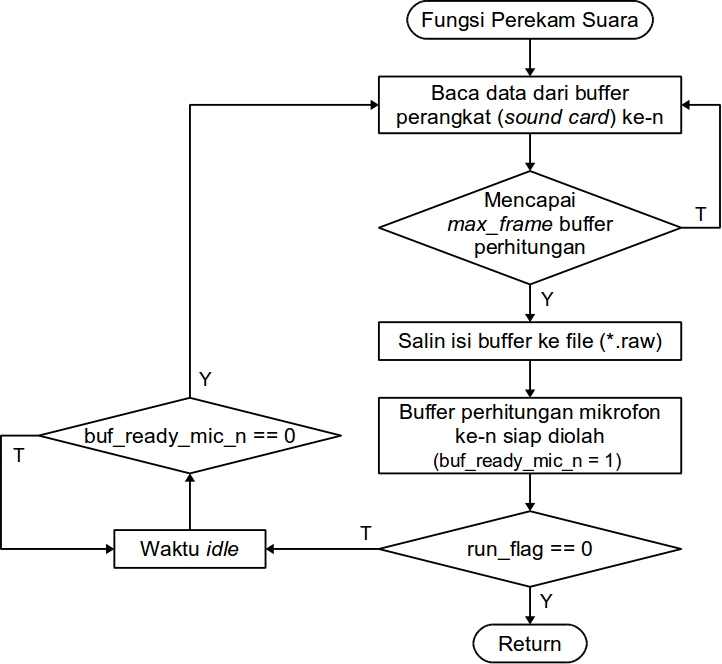
\includegraphics[scale=.5,keepaspectratio=true]{images/flowchart_record_wxspeacal.jpg}
 \caption[Diagram alir fungsi perekam suara pada SpeaCal]{Diagram alir fungsi perekam suara pada SpeaCal.}
 \label{fig:flowchart_record_wxspeacal}
\vskip .5em
\end{figure}

\begin{figure}[htp!]
\vskip 1em
\centering
 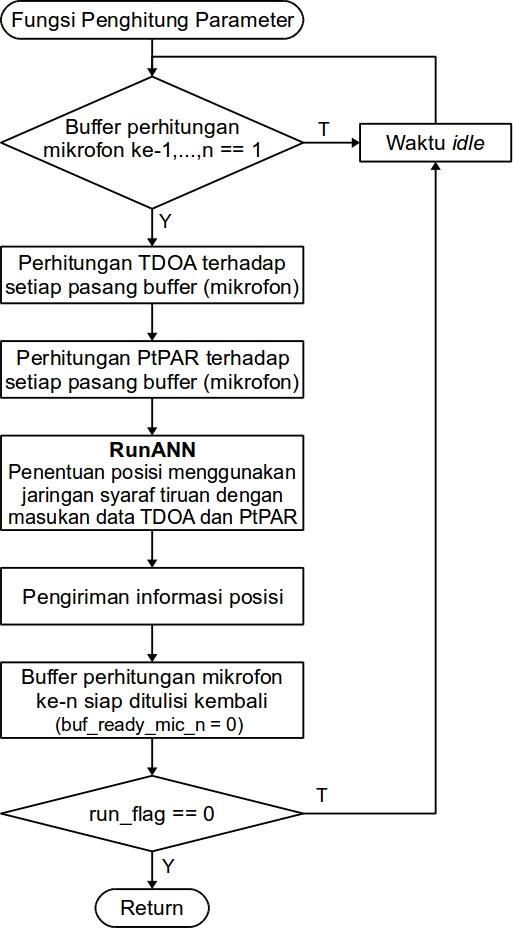
\includegraphics[scale=.5,keepaspectratio=true]{images/flowchart_compute_wxspeacal.jpg}
 \caption[Diagram alir fungsi penghitung parameter TDOA dan PtPAR pada SpeaCal]{Diagram alir fungsi penghitung parameter TDOA dan PtPAR pada SpeaCal.}
 \label{fig:flowchart_compute_wxspeacal}
\vskip .5em
\end{figure}

\begin{figure}[ht!]
\vskip 1em
\centering
 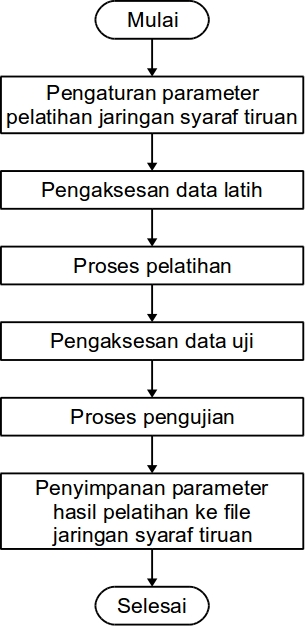
\includegraphics[scale=.5,keepaspectratio=true]{images/flowchart_main_anntraining.jpg}
 \caption[Diagram alir program untuk melatih JST]{Diagram alir program untuk melatih JST.}
 \label{fig:flowchart_main_anntraining}
\vskip .5em
\end{figure}


\subsubsection{Perangkat Keras}

Dalam penentuan posisi pengguna berdasarkan TDOA dan PtPAR, penempatan mikrofon akan sangat berpengaruh. Empat mikrofon yang digunakan akan ditempatkan pada perangkat \textit{multitouch} vertikal seperti yang ditunjukkan oleh \autoref{fig:desain_mic_1}. Dengan desain tersebut diharapkan posisi pengguna dalam ruang dapat diperkirakan. Apabila manusia dapat memperkirakan \textit{azimuth} posisi sumber suara dengan dua telinga, secara logis \textit{azimuth} posisi pengguna dapat diperkirakan dengan membandingkan sinyal yang tertangkap oleh mikrofon kanan dan kiri, sedangkan \textit{elevation} dapat diperkirakan dengan sinyal dari mikrofon atas dan bawah. Selain itu, dengan adanya perbedaan jarak mikrofon kanan-kiri dan mikrofon atas-bawah terhadap permukaan layar, diharapkan jarak pengguna terhadap layar juga dapat diperkirakan memanfaatkan parameter TDOA dan PtPAR yang membandingkan kombinasi mikrofon kanan-kiri dan mikrofon atas-bawah, misalnya parameter TDOA dan PtPAR pasangan mikrofon atas dan kanan. meskipun demikian, prioritas utama adalah memperolah \textit{azimuth} posisi pengguna relatif terhadap perangkat \textit{multitouch}.

\addtocontents{lof}{\vspace{4em} \hfill {Halaman} \par}

\begin{figure}[ht!]
\vskip 1em
  \begin{center}
    \subfigure[Tampak muka]
    {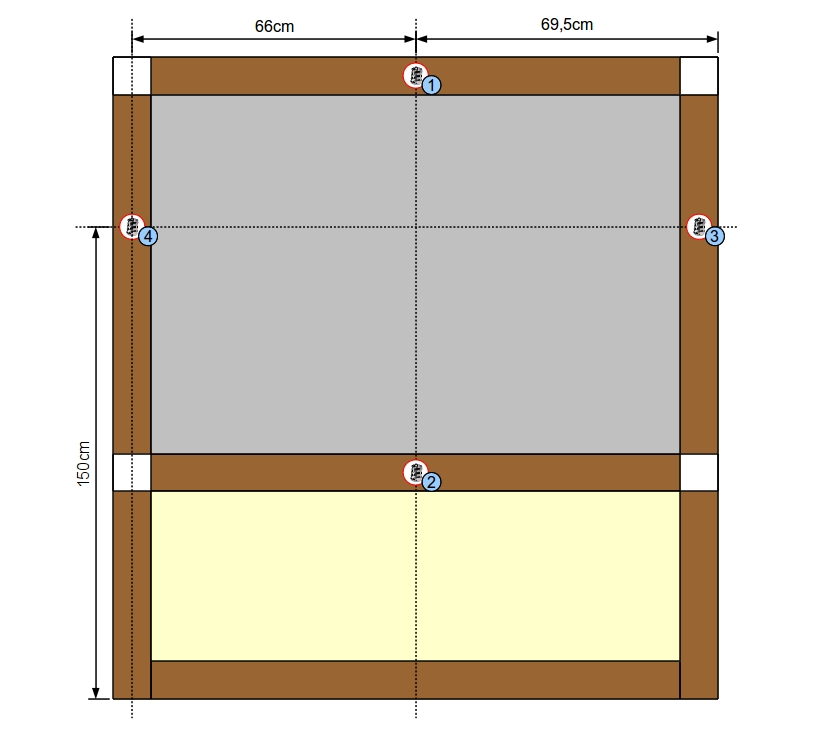
\includegraphics[scale=.5,keepaspectratio=true]{images/desain_mic_1a.jpg}
    \label{fig:desain_mic_1a}}
    \subfigure[Tampak atas]
    {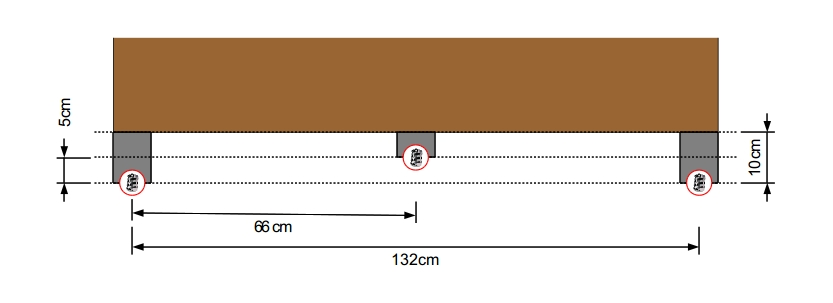
\includegraphics[scale=.5,keepaspectratio=true]{images/desain_mic_1b.jpg}
    \label{fig:desain_mic_1b}}
  \end{center}
  \caption[Rancangan penempatan mikrofon]{Rancangan penempatan mikrofon.}
  \label{fig:desain_mic_1}
  \vskip .5em
\end{figure}


\subsubsection{Pengambilan Data}

Pengambilan data latih dan uji untuk JST dilakukan dengan menempatkan sumber suara (\textit{speaker}) pada koordinat tertentu relatif terhadap perangkat \textit{multitouch} vertikal. Titik 0 dari koordinat Cartesian yang digunakan adalah ujung kiri atas perangkat \textit{multitouch}. Pengguna diasumsikan merupakan manusia dewasa dengan tinggi 160-170 cm. Dengan demikian, dapat diasumsikan bahwa posisi mulut berada pada ketinggian 150 cm dari tanah. Oleh karena itu, sumber suara ditempatkan pada koordinat $z = -30$, sedangkan koordinat $x$ dan $y$ merupakan variabel. Jangkauan nilai kedua koordinat tersebut adalah $x = \{-50, 10, 70, 130, 190\}$ dan $y = \{60, 120, 180\}$ (ditandai dengan tanda X pada \autoref{fig:floor_plan_1}).

\begin{figure}[ht!]
\vskip 1em
\centering
 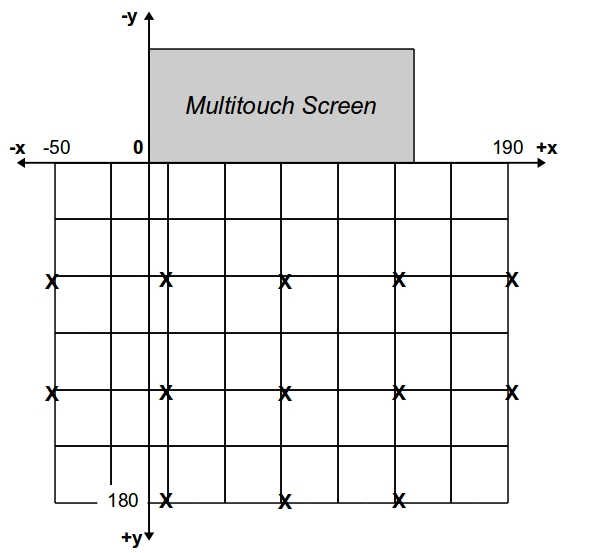
\includegraphics[scale=.5,keepaspectratio=true]{images/floor_plan_1.jpg}
 \caption[Rancangan titik pengambilan data]{Rancangan titik pengambilan data.}
 \label{fig:floor_plan_1}
\vskip .5em
\end{figure}


\subsection{Iterasi I: Implementasi}

\subsubsection{Perangkat Lunak}

Implementasi fungsi perekam suara memanfaatkan pustaka Portaudio untuk mengakses \textit{buffer} yang dimiliki \textit{sound card} dan menyalinnya ke sebuah file yang berekstensi \texttt{raw}. File-file yang berisi representasi sinyal suara dari empat mikrofon inilah yang kemudian akan diolah oleh fungsi penghitung parameter.

\singlespacing
\begin{figure}[htp!]
\vskip 1em
\begin{lstlisting}
if(inputBuffer == NULL)
{
	for(i=0; i<framesPerBuffer; i++)
    {
		output_data_buffer[i] = SAMPLE_SILENCE;  /* left */
		if(NUM_CHANNELS == 2)
			output_data_buffer[i] = SAMPLE_SILENCE;  /* right */
	}
}
else
{
	for(i=0; i<framesPerBuffer; i++)
	{
		output_data_buffer[i] = *input++;
	}
}
\end{lstlisting}
\caption[Kode program operasi pembacaan data dari \textit{buffer} yang dimiliki \textit{sound card}]{Kode program operasi pembacaan data dari \textit{buffer} yang dimiliki \textit{sound card}.}
\label{lst:read_sound_card_buffer}
\vskip .5em
\end{figure}
\onehalfspacing

\singlespacing
\begin{figure}[htp!]
\vskip 1em
\begin{lstlisting}
sprintf(recordFileName,"dev-%d-buf-rec-%d.raw", userDataFile->devNum, pubBufFileID);
buf_fid = fopen(recordFileName, "wb");
if(buf_fid == NULL)
{
	printf("Could not open file for saving the buffer.");
	exit(1);
}
else
{
	fwrite(output_data_buffer, NUM_CHANNELS * sizeof(SAMPLE), framesPerBuffer, buf_fid);
	fclose(buf_fid);
}
\end{lstlisting}
\caption[Kode program operasi penyimpanan data ke file yang berekstensi \texttt{raw}]{Kode program operasi penyimpanan data ke file yang berekstensi \texttt{raw}.}
\label{lst:save_data_to_raw_file}
\vskip .5em
\end{figure}
\onehalfspacing


Fungsi penghitung parameter terdiri dari penghitung parameter TDOA dan PtPAR. Metode CCC digunakan untuk menghitung TDOA dari sepasang data sinyal. Untuk memperoleh operasi yang cepat, metode CCC diimplentasikan menggunakan DFT. Oleh karena itu, fungsi ini memanfaatkan pustaka FFTW3 dalam proses penghitungan TDOA. \autoref{lst:ccc_op} menunjukkan implementasi metode CCC. Parameter TDOA dapat diperoleh dengan mencari nilai maksimum dari hasil operasi CCC.

\singlespacing
\begin{figure}[htp!]
\vskip 1em
\begin{lstlisting}
pa = fftw_plan_dft_1d((N << 1) - 1, signala_ext, outa, FFTW_FORWARD, FFTW_ESTIMATE);
pb = fftw_plan_dft_1d((N << 1) - 1, signalb_ext, outb, FFTW_FORWARD, FFTW_ESTIMATE);
px = fftw_plan_dft_1d((N << 1) - 1, out, out_shifted, FFTW_BACKWARD, FFTW_ESTIMATE);

for (i = 0; i < (N << 1) - 1; i++) {
	if (i < N) {
		signala_ext[i] = signala[i];
		signalb_ext[i] = signalb[i];
	}
	else {
		signala_ext[i] = 0;
		signalb_ext[i] = 0;
	}
}

fftw_execute(pa);
fftw_execute(pb);

for (i = 0; i < (N << 1) - 1; i++)
	out[i] = outa[i] * conj(outb[i]);

fftw_execute(px);

for (i = 0; i < (N << 1) - 1; i++)
	result[i] = out_shifted[(i + N) % ((N << 1) - 1)] / ((N << 1) - 1);
\end{lstlisting}
\caption[Kode program operasi CCC terhadap dua data sinyal]{Kode program operasi CCC terhadap dua data sinyal.}
\label{lst:ccc_op}
\vskip .5em
\end{figure}
\onehalfspacing


\singlespacing
\begin{figure}[htp!]
\vskip 1em
\begin{lstlisting}
maxTemp1 = minTemp1 = creal(first_xcorr_signal[0]);;
maxTemp2 = minTemp2 = creal(second_xcorr_signal[0]);

for(l = 0; l < FramesPerBuffer; l++) {
	if(creal(first_xcorr_signal[l]) > maxTemp1)
		maxTemp1 = creal(first_xcorr_signal[l]);
	if(creal(first_xcorr_signal[l]) < minTemp1)
		minTemp1 = creal(first_xcorr_signal[l]);
	if(creal(second_xcorr_signal[l]) > maxTemp2)
		maxTemp2 = creal(second_xcorr_signal[l]);
	if(creal(second_xcorr_signal[l]) < minTemp2)
		minTemp2 = creal(second_xcorr_signal[l]);
}

return 20*log10((maxTemp1-minTemp1)/(maxTemp2-minTemp2));
\end{lstlisting}
\caption[Kode program operasi perhitungan PtPAR]{Kode program operasi perhitungan PtPAR.}
\label{lst:ptpar_op}
\vskip .5em
\end{figure}
\onehalfspacing


\subsubsection{Perangkat Keras}

Implementasi rancangan penempatan mikrofon dapat dilihat pada \autoref{fig:desain_mic_1c}. Mikrofon ditancapkan pada \textit{styrofoam} yang ditempelkan pada perangkat \textit{multitouch} vertikal (\autoref{fig:desain_mic_2c2}). Selain sebagai tempat untuk meletakkan mikrofon, \textit{styrofoam} juga dapat berfungsi sebagai peredam suara. Oleh karena itu, diharapkan mikrofon hanya menangkap sinyal suara dari arah depan.

\begin{figure}[ht!]
\vskip 1em
\centering
 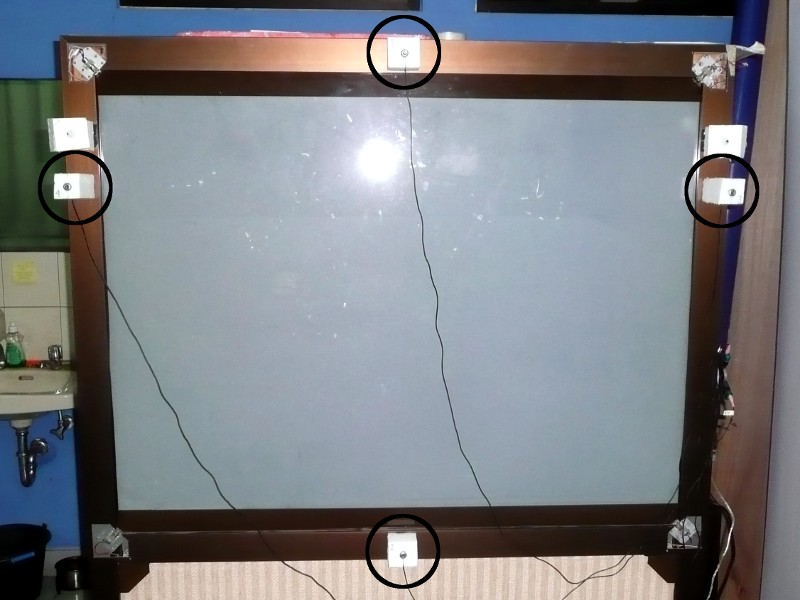
\includegraphics[width=.9\textwidth,keepaspectratio=true]{images/desain_mic_1c.jpg}
 \caption[Foto implementasi rancangan penempatan mikrofon]{Foto implementasi rancangan penempatan mikrofon.}
 \label{fig:desain_mic_1c}
\vskip .5em
\end{figure}


\subsection{Iterasi I: Pengujian dan Evaluasi}

Pengambilan data dilakukan dengan memutar secara berulang-ulang file rekaman suara FAN\_1A dan MAA\_1A yang berisi ucapan kata "satu". Masing-masing rekaman menghasilkan sebuah set data yang memuat 78 data dari 13 titik pengambilan data yang telah didefinisikan pada \autoref{subsec:iter1_desain} (6 data per titik). \autoref{fig:1_fan_1a_34}  dan \autoref{fig:1_maa_1a_34} menunjukkan parameter TDOA dan PtPAR pasangan mikrofon 3 dan 4 dari set data FAN\_1A dan MAA\_1A. Untuk memudahkan pembacaan grafik, jangkauan nilai koordinat $x = \{-50, 10, 70, 130, 190\}$ dan $y = \{60, 120, 180\}$ diubah menjadi $x = \{-2, -1, 0, 1, 2\}$ dan $y = \{-1, 0, 1\}$.

Grafik-grafik dari dua set data tersebut memperlihatkan bahwa nilai parameter PtPAR tidak cukup konsisten dan nilai parameter TDOA sangat tidak konsisten. Dua set data ini tidak dapat digunakan untuk  melatih JST yang baik.

\begin{figure}[htp!]
\vskip 1em
  \begin{center}
    \subfigure[PtPAR]
    {\fbox{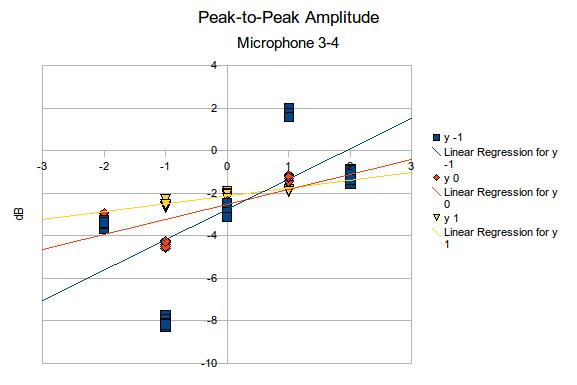
\includegraphics[scale=.55,keepaspectratio=true]{images/1_ptpar_fan_1a_34.jpg}
    \label{fig:1_ptpar_fan_1a_34}}}
    \subfigure[TDOA]
    {\fbox{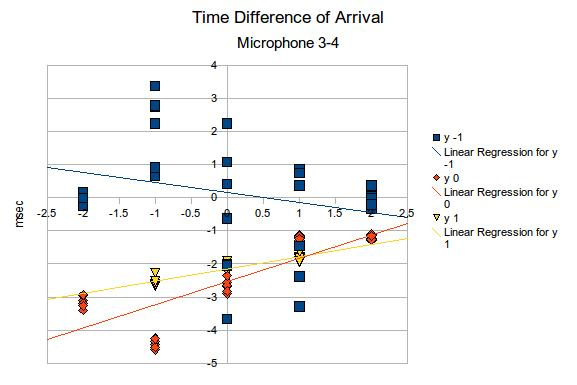
\includegraphics[scale=.55,keepaspectratio=true]{images/1_tdoa_fan_1a_34.jpg}
    \label{fig:1_tdoa_fan_1a_34}}}
  \end{center}
  \caption[Grafik TDOA dan PtPAR mikrofon 3-4 dari set data FAN\_1A]{Grafik TDOA dan PtPAR mikrofon 3-4 dari set data FAN\_1A.}
  \label{fig:1_fan_1a_34}
  \vskip .5em
\end{figure}

\begin{figure}[htp!]
\vskip 1em
  \begin{center}
    \subfigure[PtPAR]
    {\fbox{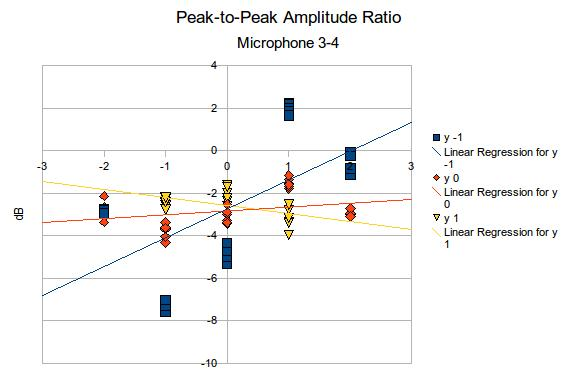
\includegraphics[scale=.55,keepaspectratio=true]{images/1_ptpar_maa_1a_34.jpg}
    \label{fig:1_ptpar_maa_1a_34}}}
    \subfigure[TDOA]
    {\fbox{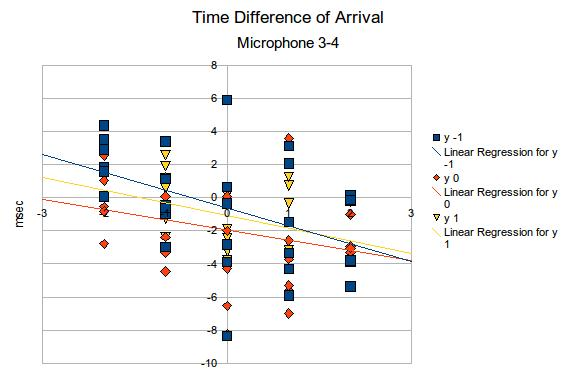
\includegraphics[scale=.55,keepaspectratio=true]{images/1_tdoa_maa_1a_34.jpg}
    \label{fig:1_tdoa_maa_1a_34}}}
  \end{center}
  \caption[Grafik TDOA dan PtPAR mikrofon 3-4 dari set data MAA\_1A]{Grafik TDOA dan PtPAR mikrofon 3-4 dari set data MAA\_1A.}
  \label{fig:1_maa_1a_34}
  \vskip .5em
\end{figure}

\subsection{Iterasi II: Desain}
\label{subsec:iter2_desain}

\subsubsection{Perangkat Keras}

Oleh karena prioritas utama adalah menentukan \textit{azimuth} posisi pengguna relatif terhadap layar, penempatan mikrofon diubah menjadi seperti yang terlihat pada \autoref{fig:desain_mic_2}. Dengan perubahan desain ini, pendekatan terhadap masalah TDOA berubah dari seperti yang tergambar pada \autoref{fig:tdoa_before} menjadi seperti yang tergambar pada \autoref{fig:tdoa_after1} dan \autoref{fig:tdoa_after2}. Selain itu, lebih banyak pasangan mikrofon yang dapat digunakan untuk memperkirakan \textit{azimuth} posisi pengguna relatif terhadap layar. Dengan demikian, terdapat enam parameter yang berpotensi sebagai masukan JST, yaitu dua nilai TDOA dari dua pasang mikrofon yang saling berdekatan dan empat nilai PtPAR dari empat pasang mikrofon yang saling berjauhan. Dua nilai PtPAR dari dua pasang mikrofon yang saling berdekatan dapat diabaikan karena perbedaan amplitudo sinyal yang tertangkap oleh sepasang mikrofon yang letaknya berdekatan tidak signifikan.

\begin{figure}[htp!]
\vskip 1em
  \begin{center}
    \subfigure[Tampak muka]
    {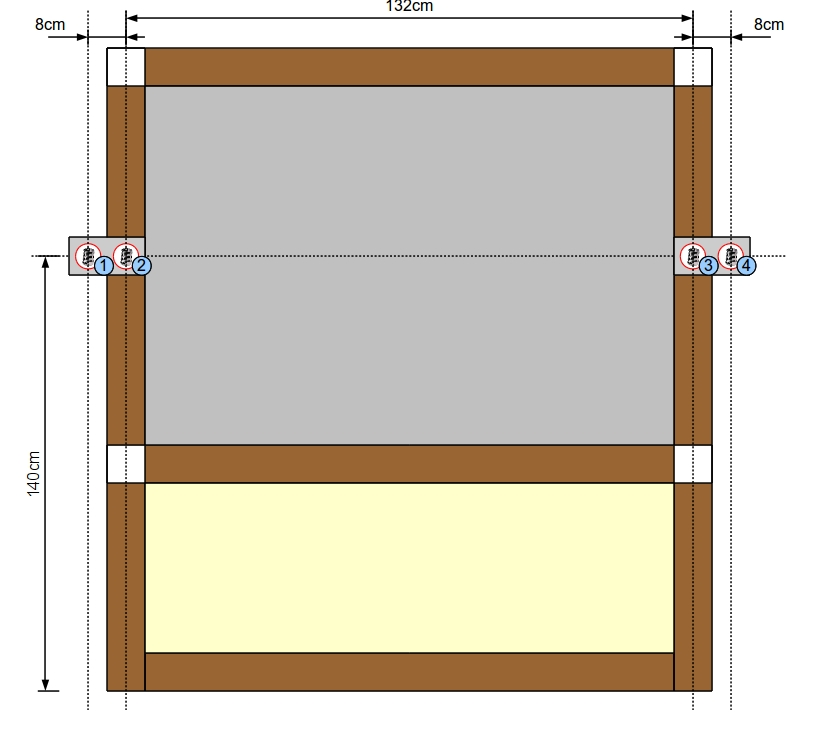
\includegraphics[scale=.5,keepaspectratio=true]{images/desain_mic_2a.jpg}
    \label{fig:desain_mic_2a}}
    \subfigure[Tampak atas]
    {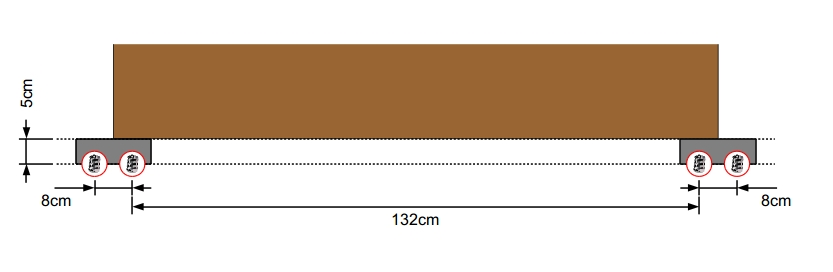
\includegraphics[scale=.5,keepaspectratio=true]{images/desain_mic_2b.jpg}
    \label{fig:desain_mic_2b}}
  \end{center}
  \caption[Perbaikan rancangan penempatan mikrofon]{Perbaikan rancangan penempatan mikrofon.}
  \label{fig:desain_mic_2}
  \vskip .5em
\end{figure}

\begin{figure}[htp!]
\vskip 1em
  \begin{center}
    \subfigure[]
    {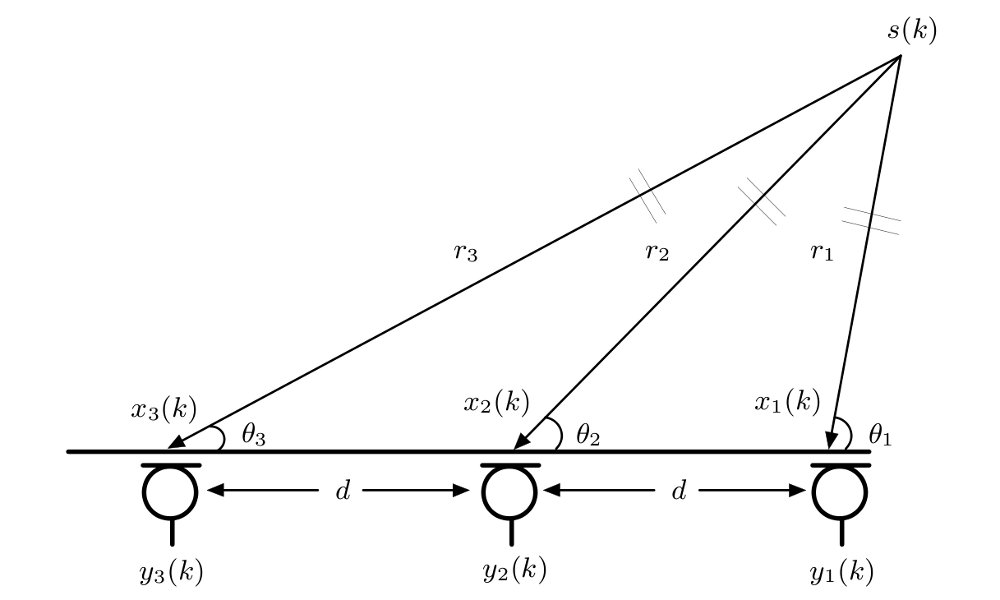
\includegraphics[scale=1.2,keepaspectratio=true]{images/tdoa_before.jpg}
    \label{fig:tdoa_before}}
    \subfigure[]
    {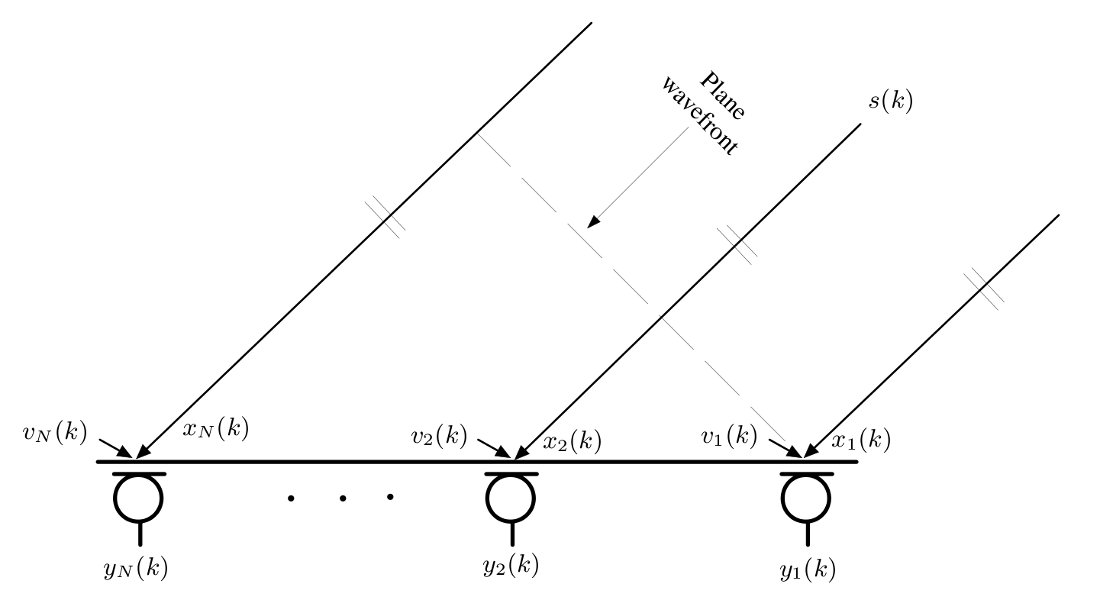
\includegraphics[scale=1.2,keepaspectratio=true]{images/tdoa_after1.jpg}
    \label{fig:tdoa_after1}}
    \subfigure[]
    {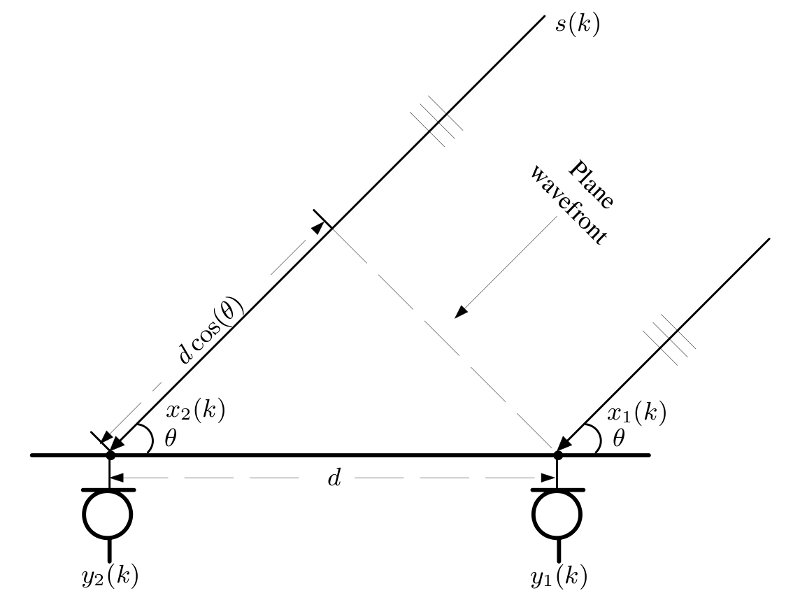
\includegraphics[scale=1.2,keepaspectratio=true]{images/tdoa_after2.jpg}
    \label{fig:tdoa_after2}}
  \end{center}
  \caption[Ilustrasi perubahan pendekatan masalah TDOA]{Ilustrasi perubahan pendekatan masalah TDOA \cite{benesty2008}.}
  \label{fig:tdoa_change}
  \vskip .5em
\end{figure}


\subsubsection{Pengambilan Data}

Jangkauan nilai koordinat sumber suara sama dengan yang digunakan sebelumnya (Iterasi I), yaitu $x = \{-50, 10, 70, 130, 190\}$, $y = \{60, 120, 180\}$, dan $z = -30$. Akan tetapi, titik-titik pengambilan data tersebut kemudian dibagi dalam kawasan-kawasan seperti yang ditunjukkan oleh \autoref{fig:floor_plan_2}. Oleh karena itu, apabila sebelumnya kemungkinan keluaran penentuan posisi pengguna adalah sebuah titik dalam koordinat Cartesian tiga dimensi yang relatif terhadap perangkat \textit{multitouch}, dengan penggunaan kawasan kemungkinan keluaran adalah sebuah sudut (\textit{azimuth}) yang relatif terhadap titik tengah perangkat \textit{multitouch}.

\begin{figure}[ht!]
\vskip 1em
\centering
 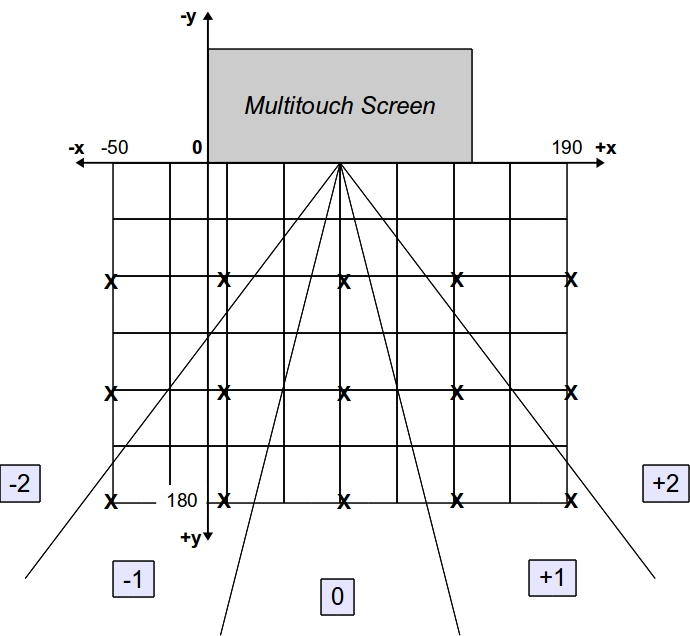
\includegraphics[scale=.5,keepaspectratio=true]{images/floor_plan_2.jpg}
 \caption[Perbaikan rancangan titik pengambilan data]{Perbaikan rancangan titik pengambilan data.}
 \label{fig:floor_plan_2}
\vskip .5em
\end{figure}

%%%%%%%%%%%%%%%%%%%%%%%%%%%%%%%%%%%%%%%%%%%%%%%%%%%%%%%%%%%%%%

\subsection{Iterasi II: Implementasi}

\subsubsection{Perangkat Keras}

Implementasi perbaikan rancangan penempatan mikrofon dapat dilihat pada \autoref{fig:desain_mic_2c1}. \autoref{fig:desain_mic_2c2} menunjukkan bagaimana mikrofon diletakkan dalam \textit{styrofoam} yang ditempelkan pada perangkat \textit{multitouch}.


\begin{figure}[ht!]
\vskip 1em
  \begin{center}
    \subfigure[]
    {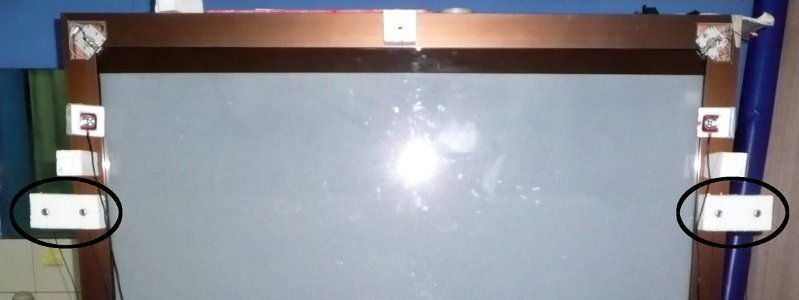
\includegraphics[width=.9\textwidth,keepaspectratio=true]{images/desain_mic_2c1.jpg}
    \label{fig:desain_mic_2c1}}
    \subfigure[]
    {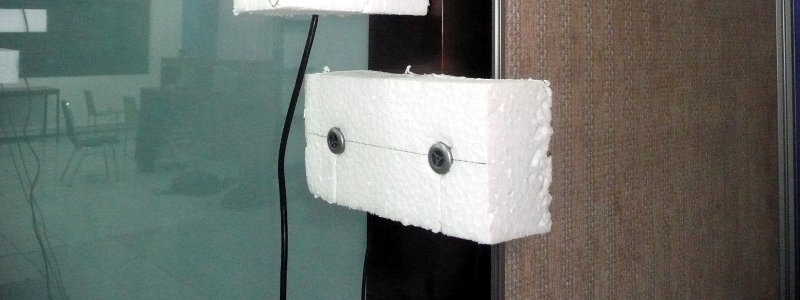
\includegraphics[width=.9\textwidth,keepaspectratio=true]{images/desain_mic_2c2.jpg}
    \label{fig:desain_mic_2c2}}
  \end{center}
  \caption[Foto implementasi perbaikan rancangan penempatan mikrofon]{Foto implementasi perbaikan rancangan penempatan mikrofon.}
  \label{fig:desain_mic_2c}
  \vskip .5em
\end{figure}

%%%%%%%%%%%%%%%%%%%%%%%%%%%%%%%%%%%%%%%%%%%%%%%%%%%%%%%%%%%%%%

\subsection{Iterasi II: Pengujian dan Evaluasi}

Dalam tahap ini, pengambilan data menggunakan empat file rekaman suara, yaitu FAN\_9B (ucapan kata "sembilan"), FAW\_7B (ucapan kata "tujuh"), MAF\_25A (ucapan frase "dua lima"), dan MSD\_5B (ucapan kata "lima"). Untuk memudahkan pembacaan grafik, jangkauan nilai koordinat $x = \{-50, 10, 70, 130, 190\}$ dan $y = \{60, 120, 180\}$ diubah menjadi $x = \{-4, -2, 0, 2, 4\}$ dan $y = \{-2, -4, -6\}$. 

Dari pengamatan terhadap empat set data, nilai parameter PtPAR cukup konsisten, sedangkan nilai parameter TDOA masih saja tidak konsisten. Dengan data tersebut, penentuan posisi pengguna diputuskan hanya akan menggunakan parameter PtPAR saja. Secara lebih spesifik, parameter PtPAR yang akan digunakan adalah parameter PtPAR mikrofon 1-3, 1-4, 2-3, dan 2-4.

Grafik TDOA dan PtPAR yang akan ditampilkan secara lengkap hanya set data FAN\_9B yang cukup merepresentasikan set data yang lain (\autoref{fig:2_fan_9b_tdoa_1} sampai dengan \autoref{fig:2_fan_9b_ptpar_3}). \autoref{fig:2_faw_7b_ptpar_1} dan \autoref{fig:2_faw_7b_ptpar_2} menunjukkan grafik PtPAR mikrofon 1-3, 1-4, 2-3, dan 2-4 dari set data FAW\_7B untuk memberikan gambaran lebih lanjut mengenai data latih dan data uji JST.

\begin{figure}[htp!]
\vskip 1em
  \begin{center}
    \subfigure[TDOA 1-2]
    {\fbox{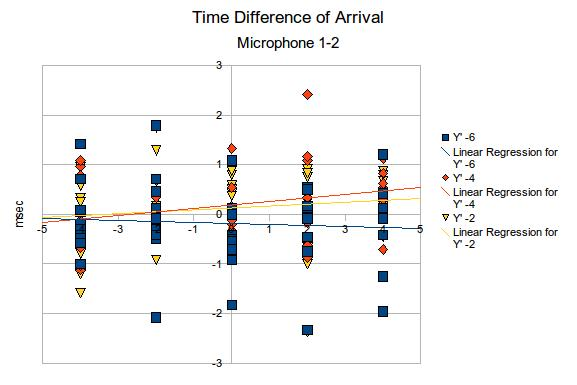
\includegraphics[scale=.55,keepaspectratio=true]{images/2_fan_9b_tdoa_12.jpg}
    \label{fig:2_fan_9b_tdoa_12}}}
    \subfigure[TDOA 3-4]
    {\fbox{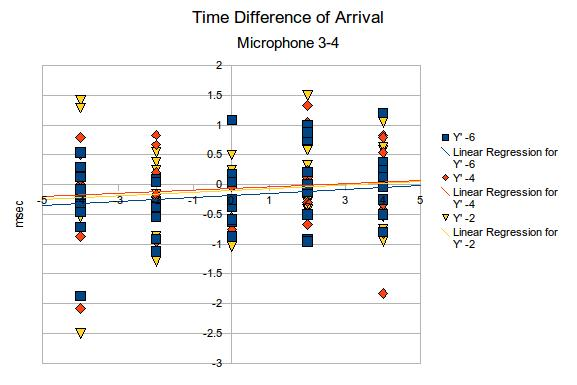
\includegraphics[scale=.55,keepaspectratio=true]{images/2_fan_9b_tdoa_34.jpg}
    \label{fig:2_fan_9b_tdoa_34}}}
  \end{center}
  \caption[Grafik TDOA dari set data FAN\_9B (1)]{Grafik TDOA dari set data FAN\_9B (1).}
  \label{fig:2_fan_9b_tdoa_1}
  \vskip .5em
\end{figure}

\begin{figure}[htp!]
\vskip 1em
  \begin{center}
    \subfigure[TDOA 1-3]
    {\fbox{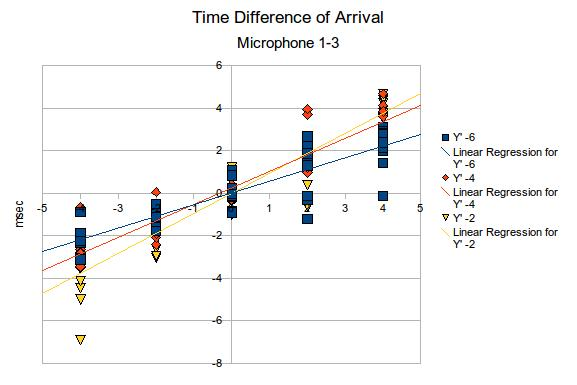
\includegraphics[scale=.55,keepaspectratio=true]{images/2_fan_9b_tdoa_13.jpg}
    \label{fig:2_fan_9b_tdoa_13}}}
    \subfigure[TDOA 1-4]
    {\fbox{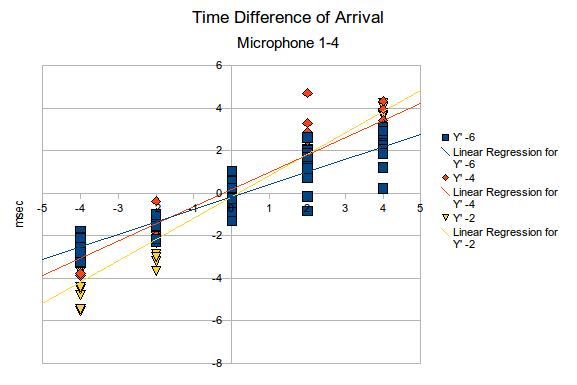
\includegraphics[scale=.55,keepaspectratio=true]{images/2_fan_9b_tdoa_14.jpg}
    \label{fig:2_fan_9b_tdoa_14}}}
  \end{center}
  \caption[Grafik TDOA dari set data FAN\_9B (2)]{Grafik TDOA dari set data FAN\_9B (2).}
  \label{fig:2_fan_9b_tdoa_2}
  \vskip .5em
\end{figure}

\begin{figure}[htp!]
\vskip 1em
  \begin{center}
    \subfigure[TDOA 2-3]
    {\fbox{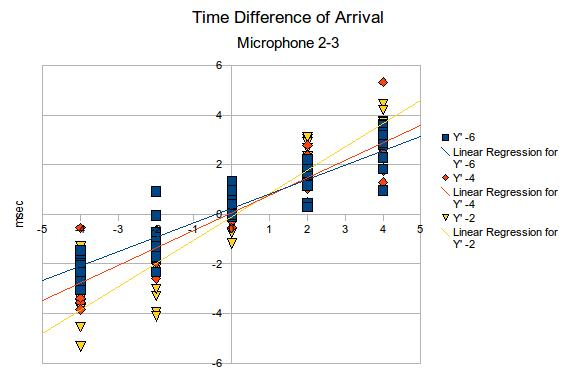
\includegraphics[scale=.55,keepaspectratio=true]{images/2_fan_9b_tdoa_23.jpg}
    \label{fig:2_fan_9b_tdoa_23}}}
    \subfigure[TDOA 2-4]
    {\fbox{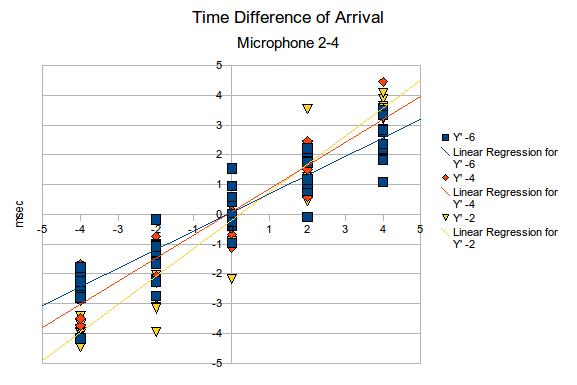
\includegraphics[scale=.55,keepaspectratio=true]{images/2_fan_9b_tdoa_24.jpg}
    \label{fig:2_fan_9b_tdoa_24}}}
  \end{center}
  \caption[Grafik TDOA dari set data FAN\_9B (3)]{Grafik TDOA dari set data FAN\_9B (3).}
  \label{fig:2_fan_9b_tdoa_3}
  \vskip .5em
\end{figure}

\begin{figure}[htp!]
\vskip 1em
  \begin{center}
    \subfigure[PtPAR 1-2]
    {\fbox{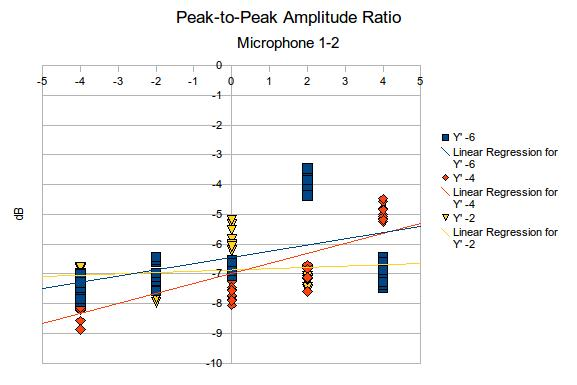
\includegraphics[scale=.55,keepaspectratio=true]{images/2_fan_9b_ptpar_12.jpg}
    \label{fig:2_fan_9b_ptpar_12}}}
    \subfigure[PtPAR 3-4]
    {\fbox{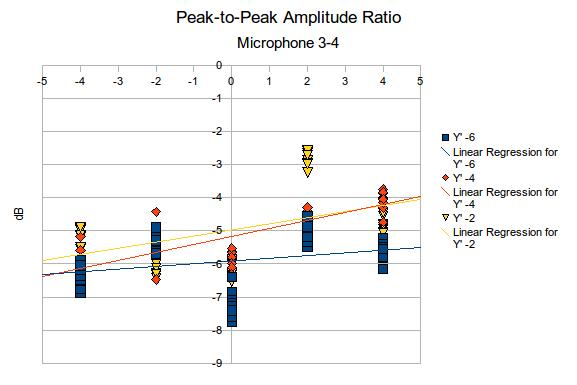
\includegraphics[scale=.55,keepaspectratio=true]{images/2_fan_9b_ptpar_34.jpg}
    \label{fig:2_fan_9b_ptpar_34}}}
  \end{center}
  \caption[Grafik PtPAR dari set data FAN\_9B (1)]{Grafik PtPAR dari set data FAN\_9B (1).}
  \label{fig:2_fan_9b_ptpar_1}
  \vskip .5em
\end{figure}

\begin{figure}[htp!]
\vskip 1em
  \begin{center}
    \subfigure[PtPAR 1-3]
    {\fbox{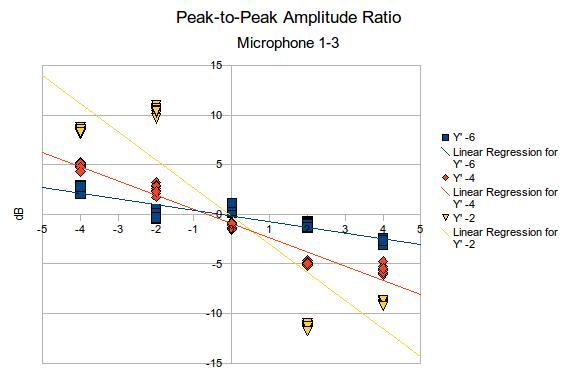
\includegraphics[scale=.55,keepaspectratio=true]{images/2_fan_9b_ptpar_13.jpg}
    \label{fig:2_fan_9b_ptpar_13}}}
    \subfigure[PtPAR 1-4]
    {\fbox{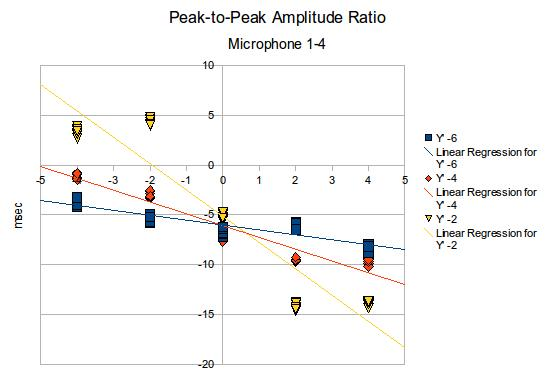
\includegraphics[scale=.55,keepaspectratio=true]{images/2_fan_9b_ptpar_14.jpg}
    \label{fig:2_fan_9b_ptpar_14}}}
  \end{center}
  \caption[Grafik PtPAR dari set data FAN\_9B (2)]{Grafik PtPAR dari set data FAN\_9B (2).}
  \label{fig:2_fan_9b_ptpar_2}
  \vskip .5em
\end{figure}

\begin{figure}[htp!]
\vskip 1em
  \begin{center}
    \subfigure[PtPAR 2-3]
    {\fbox{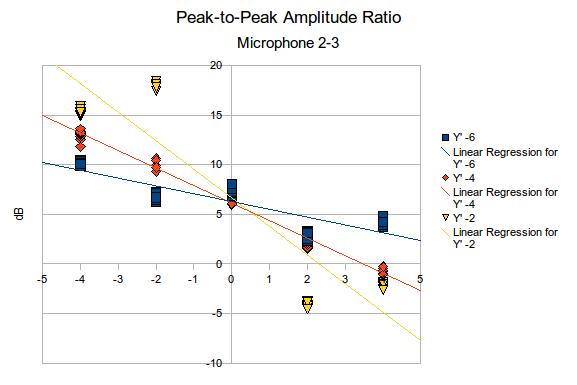
\includegraphics[scale=.55,keepaspectratio=true]{images/2_fan_9b_ptpar_23.jpg}
    \label{fig:2_fan_9b_ptpar_23}}}
    \subfigure[PtPAR 2-4]
    {\fbox{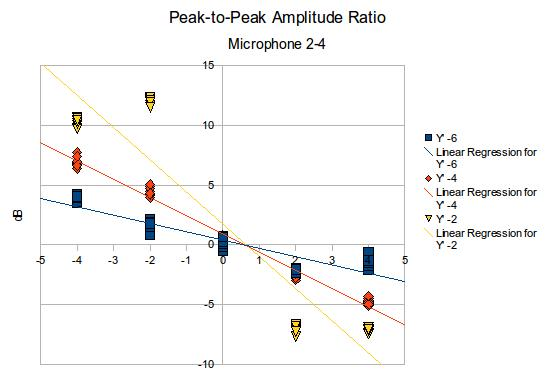
\includegraphics[scale=.55,keepaspectratio=true]{images/2_fan_9b_ptpar_24.jpg}
    \label{fig:2_fan_9b_ptpar_24}}}
  \end{center}
  \caption[Grafik PtPAR dari set data FAN\_9B (3)]{Grafik PtPAR dari set data FAN\_9B (3).}
  \label{fig:2_fan_9b_ptpar_3}
  \vskip .5em
\end{figure}

\begin{figure}[htp!]
\vskip 1em
  \begin{center}
    \subfigure[PtPAR 1-3]
    {\fbox{\includegraphics[scale=.55,keepaspectratio=true]{images/2_faw_7b_ptpar_13.jpg}
    \label{fig:2_faw_7b_ptpar_13}}}
    \subfigure[PtPAR 1-4]
    {\fbox{\includegraphics[scale=.55,keepaspectratio=true]{images/2_faw_7b_ptpar_14.jpg}
    \label{fig:2_faw_7b_ptpar_14}}}
  \end{center}
  \caption[Grafik PtPAR dari set data FAW\_7B (1)]{Grafik PtPAR dari set data FAW\_7B (1).}
  \label{fig:2_faw_7b_ptpar_1}
  \vskip .5em
\end{figure}

\begin{figure}[htp!]
\vskip 1em
  \begin{center}
    \subfigure[PtPAR 2-3]
    {\fbox{\includegraphics[scale=.55,keepaspectratio=true]{images/2_faw_7b_ptpar_23.jpg}
    \label{fig:2_faw_7b_ptpar_23}}}
    \subfigure[PtPAR 2-4]
    {\fbox{\includegraphics[scale=.55,keepaspectratio=true]{images/2_faw_7b_ptpar_24.jpg}
    \label{fig:2_faw_7b_ptpar_24}}}
  \end{center}
  \caption[Grafik PtPAR dari set data FAW\_7B (2)]{Grafik PtPAR dari set data FAW\_7B (2).}
  \label{fig:2_faw_7b_ptpar_2}
  \vskip .5em
\end{figure}



\addtocontents{toc}{\vspace{1em} \hfill {Halaman} \par}
\subsection{Pelatihan dan Pengujian Jaringan Syaraf Tiruan}

JST dilatih dengan menggunakan set data yang diperoleh pada Iterasi II. Data latih dan data uji yang digunakan berasal dari set data FAN\_9B dan FAW\_7B yang memiliki 240 data latih dan 60 data uji. Selain melakukan pelatihan dengan parameter yang sama secara berulang, parameter jumlah neuron tersembunyi dan \textit{mean squared error} (MSE) pelatihan (\textit{desired error}) juga diubah-ubah untuk memperoleh MSE pelatihan dan pengujian yang baik. Data dari proses pelatihan JST ditampilkan pada \autoref{tbl:data_pelatihan}.

JST yang diperoleh kemudian diuji dengan set data MAF\_25A dan MSD\_5B yang masing-masing memuat 50 data, serta FAN\_9B\_2 yang memuat 150 data. Data dari proses pengujian JST ditampilkan pada \autoref{tbl:data_pengujian}. Data pengujian tersebut menunjukkan bahwa MSE rata-rata terendah diperoleh dari penggunaan JST yang dihasilkan pada pelatihan ke-7. JST inilah yang nantinya akan digunakan untuk memperkirakan posisi pengguna setelah subsistem diintegrasikan ke dalam RESTU.

\begin{table}[ht!]
  \vskip 1em
\centering
\caption{Data pelatihan JST.}
\label{tbl:data_pelatihan}
\begin{tabular}{| c | c | c | c | c |}
\hline
\textbf{Pelatihan} & \textbf{Jumlah} & \textbf{Jumlah neuron} & \textbf{MSE} & \textbf{MSE} \\
\textbf{ke-} & \textbf{layer} & \textbf{tersembunyi} & \textbf{pelatihan} & \textbf{pengujian} \\
\hline
1 & 3 & 64 & 0,0009989900 & 0,010317 \\
\hline
2 & 3 & 32 & 0,0009997976 & 0,004737 \\
\hline
3 & 3 & 16 & 0,0009985201 & 0,000379 \\
\hline
4 & 3 & 16 & 0,0007484510 & 0,002396 \\
\hline
5 & 3 & 16 & 0,0004987848 & 0,004765 \\
\hline
6 & 3 & 16 & 0,0002499711 & 0,008815 \\
\hline
7 & 3 & 16 & 0,0001499649 & 0,005309 \\
\hline
8 & 3 & 16 & 0,0000999883 & 0,027223 \\
\hline
\end{tabular}
  \vskip .5em
\end{table}


\begin{table}[ht!]
  \vskip 1em
\centering
\caption{Data pengujian JST.}
\label{tbl:data_pengujian}
\begin{tabular}{| c | c | c | c | c |}
\hline
\textbf{JST Hasil} & \textbf{MSE} & \textbf{MSE} & \textbf{MSE} & \textbf{MSE} \\
\textbf{Pelatihan ke-} & \textbf{MAF\_25A} & \textbf{MSD\_5B} & \textbf{FAN\_9B\_2} & \textbf{Rata-rata} \\
\hline
1 & 0,174747 & 0,366794 & 0,309057 & 0,283533 \\
\hline
2 & 0,191638 & 0,400196 & 0,467885 & 0,353240 \\
\hline
3 & 0,201244 & 0,372975 & 0,426066 & 0,333428 \\
\hline
4 & 0,199302 & 0,219985 & 0,417764 & 0,279017 \\
\hline
5 & 0,176784 & 0,230723 & 0,445191 & 0,284233 \\
\hline
6 & 0,172334 & 0,368824 & 0,437893 & 0,326350 \\
\hline
7 & 0,139543 & 0,210295 & 0,464500 & 0,271446 \\
\hline
8 & 0,181249 & 0,356440 & 0,602393 & 0,380027 \\
\hline
\end{tabular}
  \vskip .5em
\end{table}


%%%%%%%%%%%%%%%%%%%%%%%%%%%%%%%%%%%%%%%%%%%%%%%%%%%

\subsection{Analisis Hasil}

Dari proses perancangan yang telah dilakukan, beberapa pencapaian yang telah diperoleh antara lain sebagai berikut.

\begin{enumerate}
\item Menangkap suara pengguna dengan menggunakan \textit{microphone array}, yang terdiri dari empat mikrofon, secara bersamaan memanfaatkan pustaka Portaudio. Representasi sinyal yang ditangkap disimpan dalam file yang berekstensi \texttt{raw}.
\item Menghitung TDOA dari sinyal suara yang ditangkap oleh \textit{microphone array} menggunakan metode CCC. Implementasi CCC menggunakan DFT memanfaatkan pustaka FFTW3. Implementasi telah diverifikasi kebenarannya dengan cara membandingkan hasil perhitungan yang diperoleh dari implementasi dengan hasil perhitungan yang diperoleh dari fungsi \texttt{xcorr} pada program Octave.
\item Menghitung PtPAR dari sinyal suara yang ditangkap oleh \textit{microphone array}. Implementasi telah diverifikasi kebenarannya dengan cara membandingkan hasil perhitungan yang diperoleh dari implementasi dengan hasil pengamatan grafik sinyal yang ditampilkan program Audacity.
\item Menyimpan data TDOA, PtPAR, dan posisi untuk membuat data latih dan data uji JST.
\item Melatih JST dengan nilai TDOA dan/atau PtPAR yang didapatkan selama pengambilan data latih dengan memanfaatkan pustaka FANN.
\item Menguji JST dengan nilai TDOA dan/atau PtPAR yang didapatkan selama pengambilan data uji dengan memanfaatkan pustaka FANN.
\end{enumerate}

Pada awal penelitian, parameter TDOA dan PtPAR diperkirakan dapat digunakan untuk melakukan penentuan posisi sumber suara, atau dalam hal ini adalah posisi pengguna. Parameter PtPAR terbukti dapat digunakan untuk memperkirakan posisi pengguna, sedangkan parameter TDOA tidak dapat. Meskipun demikian, parameter TDOA sebenarnya merupakan parameter yang banyak digunakan dalam penentuan posisi sumber suara sehingga tingkat keakuratannya seharusnya cukup baik. Oleh karena itu, tidak dapat digunakannya parameter tersebut dalam penelitian ini disebabkan oleh desain dan implementasi yang kurang sesuai dengan batasan masalah TDOA.

Faktor utama yang menyebabkan hasil perhitungan TDOA sangat tidak konsisten adalah faktor perangkat keras yang digunakan. Penggunaan \textit{USB sound card} yang kemudian datanya dikelola oleh program yang memanfaatkan pustaka Portaudio tidak dapat menghasilkan representasi data sinyal yang baik karena batasan waktu tidak ditepati dengan baik. Dari pengamatan, proses perekaman yang dilakukan oleh empat \textit{sound card} tidak berjalan secara bersamaan. Pengamatan dilakukan dengan memberikan penanda waktu (\textit{timestamp}) saat proses merekam mulai dan berakhir. Dari penanda waktu tersebut diketahui bahwa durasi perekaman tidak pernah terpenuhi dan durasi \textit{sound card} yang satu dengan yang lain dalam mengambil data tidak sama , meskipun semua \textit{sound card} diset untuk merekam dalam durasi yang sama. Sebagai contoh, apabila semua \textit{sound card} diset untuk merekam selama 1 detik, penanda waktu menunjukkan bahwa \textit{sound card} merekam dalam durasi $1 + \delta t$, dengan $\delta t$ bervariasi antara satu \textit{sound card} dengan \textit{sound card} yang lain. Apabila  $\delta t$ dari satu proses perekaman ke proses yang lain sama (konsisten), permasalahan mungkin dapat dipecahkan dengan memberikan \textit{offset} pada data. Dari pengamatan $\delta t$ dari satu proses perekaman ke proses yang lain tidak konsisten. meskipun nilai $\delta t$ hanya dalam orde milidetik, pada dasarnya file representasi sinyal suara yang diperoleh tidak dapat digunakan untuk menghitung TDOA. Apabila sinyal tersebut digunakan untuk menghitung TDOA, hasil perhitungan merupakan nilai yang tidak valid karena nilai tersebut sangat dipengaruhi oleh $\delta t$ sehingga tidak merepresentasikan perbedaan waktu yang dibutuhkan propagasi sinyal dari sumber suara ke mikrofon dengan baik.

Untuk memecahkan permasalahan tersebut dibutuhkan perangkat akuisisi sinyal yang mampu berjalan secara \textit{real-time}, seperti yang digunakan pada \cite{lee2005}, \cite{nakano2010}, dan \cite{park2009}. Pada prinsipnya, apabila \textit{time-constraint} yang diberikan dapat ditepati dengan baik, dengan asumsi model \textit{free-field} ideal, representasi sinyal akan memenuhi \autoref{eq:sinyal_ditangkap}.

\chapter{\uppercase{Integrasi SpeaCal dalam RESTU}}
\label{chap:integrasi}

\section{Iterasi III: Desain}

\subsubsection{Perangkat Lunak}

Subsistem penentuan posisi pengguna berdasarkan sinyal suara yang telah didesain pada \autoref{chap:perancangan} harus diintegrasikan dengan RESTU. Pada dasarnya, proses integrasi hanya mencakup proses pengiriman data hasil penentuan posisi yang dihasilkan oleh SpeaCal ke salah satu bagian dari RESTU, misalnya \textit{AI Engine} atau \textit{GUI Engine} (\autoref{fig:speacal_block_diagram}).

Pada konsep \textit{artificial general intelligence} (AGI), semua informasi yang diterima oleh agen, termasuk informasi posisi pengguna, seharusnya masuk ke \textit{AI Engine} terlebih dahulu. Oleh karena bagian kognitif dari RESTU belum menggunakan konsep AGI ini, untuk sementara informasi yang diterima oleh agen diteruskan ke bagian yang langsung membutuhkannya. Dengan demikian, informasi dari subsistem penentuan posisi pengguna berdasarkan sinyal suara dan subsistem penentuan posisi pengguna berdasarkan citra langsung dikirimkan ke \textit{GUI Engine}, tanpa melalui \textit{AI Engine} (\autoref{fig:speacal_block_diagram_rev}). Oleh karena itu, desain pengiriman data dari subsistem penentuan posisi pengguna berdasarkan sinyal suara perlu memperhatikan desain masukan data yang digunakan oleh \textit{GUI Engine}.

\begin{figure}[ht!]
\vskip 1em
\centering
 \includegraphics[width=.9\textwidth,keepaspectratio=true]{images/speacal_block_diagram_rev.jpg}
 \caption[Diagram aliran data dari SpeaCal ke \textit{GUI Engine}]{Diagram aliran data dari SpeaCal ke \textit{GUI Engine}.}
 \label{fig:speacal_block_diagram_rev}
\vskip .5em
\end{figure}

\textit{GUI Engine} akan membuka sebuah \textit{socket} untuk pengiriman data dari subsistem penentuan posisi pengguna berdasarkan sinyal suara dan subsistem penentuan posisi pengguna berdasarkan citra. Format penulisan informasi posisi dari dua subsistem tersebut dibedakan agar \textit{GUI Engine} mengetahui darimana informasi berasal. Informasi posisi kemudian dituliskan dalam format koordinat Cartesian tiga dimensi dengan urutan penulisan: koordinat $z$, $y$, kemudian $x$. (\autoref{lst:format_audio}).

\singlespacing
\begin{figure}[htp!]
\vskip 1em
\begin{lstlisting}
a|-30|120|10|
\end{lstlisting}
\caption[Contoh penulisan informasi posisi yang dikirim dari SpeaCal ke \textit{GUI Engine Server}]{Contoh penulisan informasi posisi yang dikirim dari SpeaCal ke \textit{GUI Engine Server}.}
\label{lst:format_audio}
\vskip .5em
\end{figure}
\onehalfspacing

Daerah cakupan subsistem penentuan posisi pengguna berdasarkan citra relatif sempit. Apabila mengacu pada pembagian kawasan yang digunakan oleh subsistem penentuan posisi pengguna berdasarkan sinyal suara (\autoref{fig:floor_plan_2}), subsistem penentuan posisi pengguna berdasarkan citra hanya mencakup kawasan 0 saja.

Prioritas penggunaan informasi posisi pengguna yang berdasarkan citra lebih tinggi daripada informasi yang berdasarkan sinyal suara. Hal ini dikarenakan penentuan posisi pengguna berdasarkan citra menghasilkan posisi yang lebih akurat daripada penentuan posisi berdasarkan sinyal suara. Apabila subsistem penentuan posisi pengguna berdasarkan citra menangkap posisi pengguna melalui dua \textit{webcam} yang digunakannya, \textit{GUI Engine} akan menggunakan informasi posisi dari subsistem tersebut. Apabila tidak ada informasi dari subsistem penentuan posisi berdasarkan citra, \textit{GUI Engine} akan menggunakan informasi dari subsistem penentuan posisi berdasarkan sinyal suara.

Untuk meningkatkan akurasi dalam penentuan posisi pengguna, SpeaCal melakukan tiga kali proses penentuan posisi dengan JST. Hasil dari tiga proses tersebut kemudian diurutkan untuk mencari nilai mediannya. Dengan demikian, apabila sampel sinyal suara yang digunakan untuk menentukan posisi diset $\dfrac{1}{2}$ detik, informasi posisi pengguna akan diperbarui setiap 3 detik.

Informasi posisi yang diterima oleh \textit{GUI Engine} menggunakan format koordinat Cartesian tiga dimensi. Oleh karena itu, nilai median yang diperoleh sebelumnya perlu dikonversi terlebih dahulu dari format kawasan ke format koordinat Cartesian tiga dimensi. Dalam proses konversi koordinat yang dipilih untuk merepresentasikan kawasan adalah koordinat yang terletak pada $y = 120$. Dengan kata lain, $posisi_{kawasan} = {-2, -1, 0, 1, 2}$ dikonversi menjadi $posisi_{Cartesian} = (x, 120, -30)$, dengan $x = {-50, 10, 70, 130, 190}$. Koordinat Cartesian inilah yang kemudian dikirimkan ke \textit{GUI Engine} dengan format seperti yang tercantum pada \autoref{lst:format_audio}.


%%%%%%%%%%%%%%%%%%%%%%%%%%%%%%%%%%%%%%%%%%%

\section{Iterasi III: Implementasi}

\subsubsection{Perangkat Lunak}

Implementasi konversi koordinat dari format kawasan ke format koordinat Cartesian tiga dimensi tertulis pada \autoref{lst:konversi}. Sedangkan, implementasi penyusunan data yang akan dikirimkan ke \textit{GUI Engine} sesuai format penulisan yang telah didefinisikan dan pengiriman data melalui \textit{socket} tertulis pada \autoref{lst:socket}. Dua operasi terkait \textit{socket} tersebut diimplementasikan memanfaatkan pustaka Boost.

\singlespacing
\begin{figure}[htp!]
\vskip 1em
\begin{lstlisting}
speakerPosValue[0] = annResult * 60 + 70;
speakerPosValue[1] = 120;
speakerPosValue[2] = -30;
\end{lstlisting}
\caption[Kode program operasi konversi koordinat]{Kode program operasi konversi koordinat.}
\label{lst:konversi}
\vskip .5em
\end{figure}
\onehalfspacing

\singlespacing
\begin{figure}[htp!]
\vskip 1em
\begin{lstlisting}
try
{
	boost::asio::io_service io_service;
	boost::asio::ip::tcp::resolver resolver(io_service);
	boost::asio::ip::tcp::resolver::query query(boost::asio::ip::tcp::v4(), "167.205.56.139", "12137");
	boost::asio::ip::tcp::resolver::iterator endpoint_iterator = resolver.resolve(query);
	boost::asio::ip::tcp::resolver::iterator end;
	boost::asio::ip::tcp::socket socket(io_service);
	boost::system::error_code error = boost::asio::error::host_not_found;
	while (error && endpoint_iterator != end)
	{
		socket.close();
		socket.connect(*endpoint_iterator++, error);
	}
	if (error)
		throw boost::system::system_error(error);

	std::string pos_info;
	std::string pos_data_start ("a");
	std::string pos_data_separator ("|");

	pos_info.clear();
	pos_info = pos_data_start;
	pos_info += pos_data_separator;
	pos_info += boost::lexical_cast<std::string>(speakerPosValue[2]);
	pos_info += pos_data_separator;
	pos_info += boost::lexical_cast<std::string>(speakerPosValue[1]);
	pos_info += pos_data_separator;
	pos_info += boost::lexical_cast<std::string>(speakerPosValue[0]);
	pos_info += pos_data_separator;

	try
	{
		boost::asio::write(socket, boost::asio::buffer( pos_info ));
		std::cout << pos_info << std::endl;
	}
	catch( std::exception e )
		throw std::runtime_error("message send error | " + std::string( e.what() ) );
}
catch (std::exception& e)
	std::cerr << e.what() << std::endl;
\end{lstlisting}
\caption[Kode program operasi pengiriman data dari SpeaCal ke \textit{GUI Engine} melalui \textit{socket}]{Kode program operasi pengiriman data dari SpeaCal ke \textit{GUI Engine} melalui \textit{socket}.}
\label{lst:socket}
\vskip .5em
\end{figure}
\onehalfspacing

%%%%%%%%%%%%%%%%%%%%%%%%%%%%%%%%%%%%%%%%%%%

\section{Iterasi III: Pengujian dan Evaluasi}

Pengujian menunjukkan bahwa data dari SpeaCal dapat diterima dengan baik oleh \textit{GUI Engine}. Pada saat pengujian, koneksi beberapa kali terputus karena sinyal WLAN yang lemah. Selain itu, tidak ada permasalahan yang dihadapi oleh komunikasi data antara SpeaCal dan \textit{GUI Engine}.

Setelah SpeaCal berhasil diintegrasikan dalam RESTU, pengujian pengguna secara terbatas juga dilakukan. Pengujian melibatkan pihak-pihak yang juga terlibat dalam pengembangan RESTU. Dari proses pengujian, diketahui bahwa SpeaCal dapat menghasilkan informasi posisi pengguna berdasarkan suara pengguna. Meskipun demikian, informasi posisi yang dihasilkan seringkali masih tidak akurat. Dari hasil pengamatan, hasil SpeaCal cenderung berkisar pada nilai -1, 0, dan 1, meskipun pada faktanya pengguna berada pada kawasan -2 atau 2. SpeaCal akan menghasilkan nilai -2 atau 2 apabila jarak pengguna relatif sangat dekat dengan salah satu pasangan mikrofon.

Pengujian menunjukkan bahwa SpeaCal menghasilkan perkiraan posisi yang lebih akurat apabila pengguna memperbesar amplitudo suaranya dengan sedikit berteriak. Selain itu, SpeaCal sensitif terhadap suara yang bersifat \textit{spike}, misalnya suara tepukan tangan dan suara jentikan jari.

Pengujian juga menunjukkan bahwa SpeaCal sangat sensitif terhadap derau. Pada awal pengujian, sebuah \textit{server} diletakkan di samping perangkat \textit{multitouch}, di bawah mikrofon 1-2. Dalam kondisi ini, SpeaCal memiliki kecenderungan menunjukkan nilai -1, bahkan saat tidak ada suara yang dominan di ruangan. Ketika posisi \textit{server} sedikit dimundurkan, kecenderungan menunjukkan nilai -1 berkurang dan SpeaCal kembali menunjukkan nilai 0 saat tidak ada suara pengguna.



%%%%%%%%%%%%%%%%%%%%%%%%%%%%%%%%%%%%%%%%%%%

\section{Analisis Hasil}

Dari proses perancangan lanjutan yang telah dilakukan, beberapa tambahan pencapaian yang telah diperoleh antara lain sebagai berikut.

\begin{enumerate}
\item Menggunakan JST untuk menghasilkan informasi perkiraan posisi pengguna (sumber suara) secara \textit{real-time}, meskipun hasilnya seringkali masih tidak akurat.
\item Mengirimkan informasi perkiraan posisi pengguna ke bagian \textit{GUI Engine} dari RESTU yang kemudian dimanfaatkan untuk menentukan ke arah mana agen virtual menengokkan kepalanya.
\end{enumerate}

Hasil penentuan posisi yang seringkali tidak akurat mungkin disebabkan oleh sensitivitas mikrofon yang kurang memadai. Hal ini ditandai oleh penentuan posisi sering menunjukkan hasil yang akurat apabila penguji (pengguna) mengeluarkan suara yang beramplitudo yang lebih besar dibandingkan dengan saat berbicara normal.

Kurang akuratnya penentuan posisi berdasarkan sinyal suara juga dipengaruhi oleh derau suara yang ada saat penggunaan. Saat sebuah komputer salah satu \textit{server} RESTU diletakkan di bawah mikrofon 1-2, hasil penentuan posisi cenderung menunjukkan nilai -1. Bahkan, dalam kondisi tidak ada pengguna yang bersuara, SpeaCal menunjukkan nilai -1. Hal ini menunjukkan bahwa suara kipas dari komputer tersebut menjadi derau bagi SpeaCal. Dengan demikian, mengganti mikrofon dengan yang lebih baik pun tidak cukup untuk meningkatkan akurasi SpeaCal karena dengan mikrofon yang lebih sensitif berarti semakin banyak pula derau yang tertangkap.

Alternatif solusi yang lain adalah menambahkan operasi pra-pemrosesan sinyal. Sebagai contoh, penggunaan \textit{filter} dimungkinkan untuk memperkecil pengaruh derau yang potensial ada di lingkungan penggunaan RESTU, misalnya derau kipas komputer. Sebenarnya SpeaCal telah mengimplementasikan \textit{biquad band-pass filter} untuk jangkauan frekuensi 300-3300 Hz yang merupakan jangkauan frekuensi suara manusia. Akan tetapi, tampaknya penggunaan \textit{filter} tersebut saja tidak cukup untuk menghasilkan penentuan posisi pengguna yang baik.

Salah satu batasan masalah dalam penelitian ini adalah hanya ada satu sumber suara (pengguna). Di luar batasan tersebut, potensi derau yang terbesar dari SpeaCal adalah suara manusia yang statusnya bukan pengguna. Alternatif solusi dari permasalahan ini adalah pengembangan subsistem penentuan posisi pengguna berdasarkan audiovisual yang mengintegrasikan proses penentuan posisi berdasarkan sinyal suara dan citra, tidak hanya mengombinasikan hasil dari dua proses penentuan posisi berdasarkan sinyal suara dan citra yang terpisah.

\chapter{\uppercase{Kesimpulan dan Saran}}
\label{chap:kesimpulan}

%%%%%%%%%%%%%%%%%%%%%%%%%%%%%%%%

\section{Kesimpulan}

SpeaCal yang merupakan subsistem penentuan posisi pengguna berdasarkan sinyal suara untuk RESTU telah berhasil dirancang, diimplementasikan, diuji, dan diintegrasikan dalam RESTU. SpeaCal telah memenuhi kebutuhan subsistem ini, yaitu memberikan informasi perkiraan \textit{azimuth} posisi pengguna relatif terhadap layar.

SpeaCal telah memenuhi spesifikasi yang sebelumnya didefinisikan, dengan detail sebagai berikut.

\begin{enumerate}
\item SpeaCal mampu menangkap suara pengguna dengan menggunakan \textit{microphone array}, yang terdiri dari empat mikrofon, secara bersamaan memanfaatkan pustaka Portaudio. Representasi sinyal yang ditangkap disimpan dalam file yang berekstensi \texttt{raw}.
\item SpeaCal mampu menghitung TDOA dari sinyal suara yang ditangkap oleh \textit{microphone array} menggunakan metode CCC. Implementasi CCC menggunakan DFT memanfaatkan pustaka FFTW3. Implementasi telah diverifikasi kebenarannya dengan cara membandingkan hasil perhitungan yang diperoleh dari implementasi dengan hasil perhitungan yang diperoleh dari fungsi \texttt{xcorr} pada program Octave.
\item SpeaCal mampu menghitung PtPAR dari sinyal suara yang ditangkap oleh \textit{microphone array}. Implementasi telah diverifikasi kebenarannya dengan cara membandingkan hasil perhitungan yang diperoleh dari implementasi dengan hasil pengamatan grafik sinyal yang ditampilkan program Audacity.
\item SpeaCal mampu menyimpan data TDOA, PtPAR, dan posisi untuk membuat data latih dan data uji JST.
\item SpeaCal mampu melatih JST dengan nilai TDOA dan/atau PtPAR yang didapatkan selama pengambilan data latih dengan memanfaatkan pustaka FANN.
\item SpeaCal mampu menguji JST dengan nilai TDOA dan/atau PtPAR yang didapatkan selama pengambilan data uji dengan memanfaatkan pustaka FANN.
\item SpeaCal mampu menggunakan JST untuk menghasilkan informasi perkiraan posisi pengguna (sumber suara) secara riil, meskipun hasilnya seringkali masih tidak akurat.
\item SpeaCal mampu mengirimkan informasi perkiraan posisi pengguna ke bagian \textit{GUI Engine} dari RESTU yang kemudian dimanfaatkan untuk menentukan ke arah mana agen virtual menengokkan kepalanya.
\end{enumerate}

Pada awal penelitian, parameter TDOA dan PtPAR diperkirakan dapat digunakan untuk melakukan penentuan posisi sumber suara, atau dalam hal ini adalah posisi pengguna. Parameter PtPAR terbukti dapat digunakan untuk memperkirakan posisi pengguna, sedangkan parameter TDOA tidak dapat digunakan karena syarat \textit{time-constraint} tidak dapat terpenuhi oleh desain dan implementasi yang digunakan. Oleh karena itu, SpeaCal hanya menggunakan PtPAR untuk memperkirakan posisi pengguna.

JST terbaik yang diperoleh dalam proses pelatihan memiliki tiga lapisan (terdiri dari satu masukan, satu tersembunyi, dan satu keluaran) dengan 16 neuron tersembunyi. MSE pelatihan dan pengujian JST tersebut mencapai 0,0001499649 dan 0,005309. Sedangkan, pengujian dengan tiga set data lain terhadap JST tersebut menghasilkan MSE 0,139543; 0,210295; dan 0,464500.


%%%%%%%%%%%%%%%%%%%%%%%%%%%%%%%%%%

\section{Saran}

Beberapa alternatif pengembangan subsistem penentuan posisi pengguna berdasarkan sinyal pengguna yang mungkin dilakukan adalah sebagai berikut.

\begin{itemize}
\item Penggunaan perangkat keras akuisisi sinyal yang mampu berjalan secara \textit{real-time}, misalnya sistem \textit{embedded}.
\item Penambahan operasi pra-pemrosesan sinyal, misalnya penapisan derau.
\item Pengembangan ke arah penentuan posisi pengguna berdasarkan audiovisual.
\item Penggunaan model propagasi sinyal suara \textit{reverberant}.
\end{itemize}


%%%
% Daftar Pustaka
%%%

\newpage
\phantomsection \label{daftarpustaka}
\renewcommand{\bibname}{\uppercase{Daftar Pustaka}}
\addcontentsline{toc}{chapter}{\bibname}
%%%
%% This is file `merlin.tex',
%% generated with the docstrip utility.
%%
%% The original source files were:
%%
%% merlin.mbs  (with options: `bblbst')
%% 
%% IMPORTANT NOTICE:
%% 
%% For the copyright see the source file.
%% 
%% Any modified versions of this file must be renamed
%% with new filenames distinct from merlin.tex.
%% 
%% For distribution of the original source see the terms
%% for copying and modification in the file merlin.mbs.
%% 
%% This generated file may be distributed as long as the
%% original source files, as listed above, are part of the
%% same distribution. (The sources need not necessarily be
%% in the same archive or directory.)
%% Copyright 1994-2007 Patrick W Daly
 % ===============================================================
 % IMPORTANT NOTICE:
 % This bibliographic style (bst) file has been generated from one or
 % more master bibliographic style (mbs) files, listed above.
 %
 % This generated file can be redistributed and/or modified under the terms
 % of the LaTeX Project Public License Distributed from CTAN
 % archives in directory macros/latex/base/lppl.txt; either
 % version 1 of the License, or any later version.
 % ===============================================================
 % Name and version information of the main mbs file:
 % \ProvidesFile{merlin.mbs}[2007/04/24 4.20 (PWD, AO, DPC)]
 % This is babelbst.tex for English.
 % It should serve as a model for other languages.
 % Alternatively, store it under a different name (e.g. englbst.tex)
 % and then \input it with a command in babelbst.tex.
\def\bbland{dan}                \def\bbletal{et~al.}
\def\bbleditors{editor}         \def\bbleds{ed.}
\def\bbleditor{editor}          \def\bbled{ed.}
\def\bbledby{diedit oleh}
\def\bbledition{edisi}          \def\bbledn{ed.}
\def\bblvolume{volume}          \def\bblvol{vol.}
\def\bblof{dari}
\def\bblnumber{nomor}           \def\bblno{no.}
\def\bblin{dalam}
\def\bblpages{halaman}          \def\bblpp{hlm.}
\def\bblpage{halaman}           \def\bblp{hlm.}
\def\bbleidpp{halaman}
\def\bblchapter{bab}            \def\bblchap{bab}
\def\bbltechreport{Technical Report}
\def\bbltechrep{Tech. Rep.}
\def\bblmthesis{Tesis Master}
\def\bblphdthesis{Disertasi Doktor}
\def\bblfirst{Pertama}          \def\bblfirsto{Ke-1}
\def\bblsecond{Kedua}           \def\bblsecondo{Ke-2}
\def\bblthird{Ketiga}           \def\bblthirdo{Ke-3}
\def\bblfourth{Keempat}         \def\bblfourtho{Ke-4}
\def\bblfifth{Kelima}           \def\bblfiftho{Ke-5}
\def\bblst{st}  \def\bblnd{nd}  \def\bblrd{rd}
\def\bblth{th}
\def\bbljan{Januari}  \def\bblfeb{Februari}  \def\bblmar{Maret}
\def\bblapr{April}    \def\bblmay{Mei}       \def\bbljun{Juni}
\def\bbljul{Juli}     \def\bblaug{Agustus}   \def\bblsep{September}
\def\bbloct{Oktober}  \def\bblnov{November}  \def\bbldec{Desember}
\endinput
%%
%% End of file `merlin.tex'.

%\bibliographystyle{bib/el-itb}
%\bibliography{Thesis}
\singlespacing
\setlength{\parskip}{.5em}
\begin{thebibliography}{10}
\def\enquote#1{``#1''}
\expandafter\ifx\csname url\endcsname\relax
  \def\url#1{{\tt #1}}\fi
\expandafter\ifx\csname urlprefix\endcsname\relax\def\urlprefix{URL }\fi

\bibitem{baken1999}
Baken, R.~J. dan Orlikoff, R.~F.,
  {\em {Clinical Measurement of Speech \& Voice}\/},
  edisi ke-2, Singular, 1999.

\bibitem{benesty2008}
Benesty, J., Chen, J., dan Huang, Y.,
  {Direction-of-Arrival and Time-Difference-of-Arrival Estimation},
  {\em {Microphone Array Signal Processing}\/},
  181--215, Springer, 2008.

\bibitem{beun2003}
Beun, R., Vos, E.~D., dan Witteman, C.,
  {Embodied Conversational Agents: Effects on Memory Performance and Anthropomorphisation},
  {\em Intelligent Virtual Agents\/}, 
  315--319, Springer, 2003.

\bibitem{birchfield2005}
Birchfield, S. dan Gangishetty, R.,
  {Acoustic localization by interaural level difference},
  {\em Proceedings of IEEE International Conference
  on Acoustics, Speech, and Signal Processing (ICASSP'05)\/},
  \textbf{4}, IEEE, 2005.

\bibitem{cassell2000}
Cassell, J.,
  {Embodied conversational interface agents},
  {\em Communications of the ACM\/}, \textbf{43}(4),
  70--78, 2000.

\bibitem{cassell2000a}
Cassell, J., Bickmore, T., Vilhj{\'a}lmsson, H., dan Yan, H.,
  {More than just a pretty face: affordances of embodiment},
  {\em Proceedings of the 5th International Conference on Intelligent User Interfaces\/},
  52--59, ACM, 2000.

\bibitem{cassell1998}
Cassell, J., et~al.,
  {An architecture for embodied conversational characters},
  {\em Proceedings of the First Workshop on Embodied Conversational Characters\/},
  109--120, 1998.

\bibitem{cassell1999}
Cassell, J., et~al.,
  {Embodiment in conversational interfaces: Rea},
  {\em Proceedings of the SIGCHI Conference on Human Factors in Computing Systems\/},
  520--527, 1999.

\bibitem{chen2004}
Chen, J., Huang, Y.~A., dan Benesty, J.,
  {Time Delay Estimation},
  {\em {Audio Signal Processing for Next-Generation Multimedia Communication Systems}\/},
  Kluwer Academic Publishers, 2004.

\bibitem{cole1997}
Cole, R.~A., Mariani, J., Uszkoreit, H., Zaenen, A., dan Zue, V. (editor),
  {\em {Survey of State of the Art in Human Language Technology}\/},
  Cambrige University Press, 1997, \urlprefix\url{http://cslu.cse.ogi.edu/HLTsurvey/}.

\bibitem{forouzan2003}
Forouzan, B.~A.,
  {\em {Data Communications and Networking}\/}, edisi ke-3,
  McGraw-Hill, 2003.

\bibitem{foster2007}
Foster, M.,
  {Enhancing human-computer interaction with embodied conversational agents},
  {\em Universal Access in Human-Computer Interaction. Ambient Interaction\/},
  828--837, 2007.

\bibitem{gasperis2010}
Gasperis, G.~D.,
  {Building an AIML Chatter Bot Knowledge-Base Starting from a FAQ and a Glossary},
  {\em Journal of e-Learning and Knowledge Society\/}, \textbf{6}(2),
  75--83, 2010.

\bibitem{gelfand2010}
Gelfand, S.~A.,
  {\em {Hearing: An Introduction to Psychological and Physiological Acoustics}\/},
  edisi ke-5, Informa Healthcare, 2010.

\bibitem{goldstein2010}
Goldstein, E.~B.,
  {\em {Sensation and Perception}\/},
  edisi ke-8, Wadsworth, 2010.

\bibitem{halliday2004}
Halliday, D., Resnick, R., dan Walker, J.,
  {\em {Fundamentals of Physics}\/},
  edisi ke-7, Wiley, 2004.

\bibitem{hartmann2005}
Hartmann, B., Mancini, M., dan Pelachaud, C.,
  Implementing expressive gesture synthesis for embodied conversational agents,
  {\em Gesture Workshop\/}, 188--199, Springer, 2005. 

\bibitem{huang2001}
Huang, X., Acero, A., dan Hon, H.-W.,
  {\em {Spoken Language Processing: A Guide to Theory, Algorithm, and System Development}\/},
  edisi ke-1, Prentice Hall, 2001.

\bibitem{huang2008}
Huang, Y.~A., Benesty, J., dan Chen, J.,
  {Time Delay Estimation and Source Localization},
  {\em {Springer Handbook of Speech Processing}\/},
  Benesty, J., Sondhi, M.~M., dan Huang, Y.~A., editor,
  1043--1063, Springer, 2008.

\bibitem{jurafsky2009}
Jurafsky, D. dan Martin, J.~H.,
  {\em {Speech and Language Processing}\/},
  edisi ke-2, Prentice-Hall, 2009.

\bibitem{kollmeier2008}
Kollmeier, B., Brand, T., dan Meyer, B.,
  {Perception of Speech and Sound},
  {\em {Springer Handbook of Speech Processing}\/},
  Benesty, J., Sondhi, M.~M., dan Huang, Y.~A., editor, 
  61--82, Springer, 2008.

\bibitem{lee2005}
Lee, J., Ji, S., Hahn, M., dan Cho, Y.,
  {Real-Time Sound Localization Using Time Difference for Human-Robot Interaction},
  {\em Proceedings of 16th IFAC World Congress\/}, 2005.

\bibitem{lee2002}
Lee, S., Badler, J., dan Badler, N.,
  {Eyes alive},
  {\em ACM Transactions on Graphics (TOG)\/},
  \textbf{21}, 637--644, ACM, Juli 2002.

\bibitem{loebner2011}
Loebner, H.~G.,
  {\em Home Page of The Loebner Prize in Artificial Intelligence\/},
  \urlprefix\url{http://www.loebner.net/Prizef/loebner-prize.html},
  diakses pada 10 Mei 2011, 02:00 WIB.

\bibitem{martin2001}
Martin, A.~F. dan Przybocki, M.~A.,
  Speaker recognition in a multi-speaker environment,
  {\em EUROSPEECH-2001\/}, 787-790, 2001.

\bibitem{massaro2006}
Massaro, D., Liu, Y., Chen, T., dan Perfetti, C., 
  {A multilingual embodied conversational agent for tutoring speech and language learning},
  {\em Proceedings of the Ninth International Conference on Spoken Language Processing
  (Interspeech 2006-ICSLP)\/}, 825--828, 2006.

\bibitem{mctear2002}
McTear, M.~F.,
  {Spoken dialogue technology: enabling the conversational user interface,}
  {\em ACM Computing Surveys\/}, \textbf{34}, 90--169, Maret 2002.

\bibitem{morency2006}
Morency, L.-P., Christoudias, C.~M., dan Darrell, T.,
  {Recognizing gaze aversion gestures in embodied conversational discourse},
  {\em Proceedings of the 8th international conference on Multimodal interfaces\/},
  289--294, ACM, 2006.

\bibitem{nakano2010}
Nakano, A.~Y.,
  {\em Exploring {Spatial Information For Distant Speech Recognition Under
  Real Environmental Conditions}\/}, Disertasi Doktor,
  Toyohashi University of Technology, Maret 2010.

\bibitem{niewiadomski2009}
Niewiadomski, R., Bevacqua, E., Mancini, M., dan Pelachaud, C.,
  {Greta: an interactive expressive ECA system,}
  {\em Proceedings of The 8th International Conference on Autonomous Agents and
  Multiagent Systems - Volume 2\/}, 1399--1400,
  International Foundation for Autonomous Agents and Multiagent Systems, 2009.

\bibitem{nugraha2010}
Nugraha, A.~A., Taufiq, A., Utama, N.~I., dan Prihatmanto, A.~S.,
  {Smart Assistant for Museum's Objects Navigation (SAMsON)},
  {\em Proceedings of The 5th AOTULE International Postgraduate
  Students Conference on Engineering\/}, 186--189, November 2010.

\bibitem{park2009}
Park, Y.,
  {Application of 3D sound technology to intelligent robots},
  {\em Proceedings of the 3rd International Universal Communication Symposium
  on - IUCS '09\/}, 199--204, 2009.

\bibitem{rabiner2007}
Rabiner, L.~R. dan Schafer, R.~W.,
  {Introduction to digital speech processing,}
  {\em Foundations and Trends in Signal Processing\/}, \textbf{1}(1-2),
  January 2007.

\bibitem{rehm2005}
Rehm, M.,
  {From Chatterbots to Natural Interaction -- 
  Face to Face Communication with Embodied Conversational Agents},
  {\em IEICE Transactions on Information and Systems\/}, \textbf{E88-D}(11),
  2445--2452, November 2005.

\bibitem{rickel2002}
Rickel, J., Marsella, S., Gratch, J., Hill, R., Traum, D., dan Swartout, W.,
  {Toward a new generation of virtual humans for interactive experiences},
  {\em IEEE Intelligent Systems\/}, \textbf{17}(4), 32--38, Juli 2002.

\bibitem{shawar2007}
Shawar, B.~A. dan Atwell, E.,
  {Chatbots: Are they Really Useful?}
  {\em LDV Forum\/}, \textbf{22}(1), 29--49, 2007.

\bibitem{stephens-}
Stephens, K.~R.,
  {What Has the Loebner Contest Told Us About Conversant Systems?}
  \urlprefix\url{http://www.behavior.org/resources/325.pdf}, diakses
  pada 10 Mei 2011, 02:00 WIB.

\bibitem{swartout2010}
Swartout, W., et~al.,
  Ada and grace: toward realistic and engaging virtual museum guides,
  {\em Proceedings of the 10th international conference on Intelligent virtual agents (IVA'10)\/},
  286--300, Springer-Verlag, 2010.

\bibitem{turing1950}
Turing, A.~M.,
  {Computing Machinery and Intelligence}, {\em Mind\/},
  \textbf{59}(236), 433--460, Oktober 1950.

\bibitem{vanes2002}
{Van Es}, I., Heylen, D., {Van Dijk}, B., dan Nijholt, A.,
  {Making agents gaze naturally-Does it work?}
  {\em Proceedings of the Working Conference on Advanced Visual Interfaces\/},
  357--358, ACM, 2002.

\bibitem{wallace2003}
Wallace, R.~S.,
  {\em The Elements of AIML Style\/}, Maret 2003.

\bibitem{wallace2009}
Wallace, R.~S.,
  {The Anatomy of A.L.I.C.E.},
  {\em {Parsing the Turing Test}\/},
  Epstein, R., Roberts, G., dan Beber, G., editor,
  181--210, Springer, 2009.

\bibitem{weizenbaum1966}
Weizenbaum, J.,
  {ELIZA}-a computer program for the study of natural
  language comunication between man and machine,
  {\em Communications of the ACM\/}, \textbf{9}(1), 36--45, 1966.

\bibitem{alice2011}
\underline{\hspace{5em}}, {\em Chat Robot Survey\/}, {ALICE Artificial Intelligence Foundation},
  \urlprefix\url{http://www.alicebot.org/aimlbots.html}, diakses pada 10 Mei 2011, 02:00 WIB.

\bibitem{bps2010}
\underline{\hspace{5em}}, {\em Hasil Sensus Penduduk 2010: Data Agregat per Provinsi\/},
  {Badan Pusat Statistik}, 2010.

\bibitem{dppobappenas2009}
\underline{\hspace{5em}}, {\em Jumlah Pengunjung Museum di Indonesia\/},
  {Direktorat Kebudayaan, Pariwisata, Pemuda, dan Olahraga, Badan Perencanaan Pembangunan Nasional}, 2009,
  \urlprefix\url{http://kppo.bappenas.go.id/preview/225}, diakses pada 10 Mei 2011, 17:00 WIB.
  
\bibitem{themuseumofscienceboston-}
\underline{\hspace{5em}}, {\em Meet Ada and Grace: Virtual Museum Guides\/},
  {The Museum of Science, Boston}, \urlprefix\url{http://www.mos.org/interfaces/adagrace.php},
  diakses pada 10 Mei 2011, 17:00 WIB.

\bibitem{uscinstituteforcreativetechnologies-}
\underline{\hspace{5em}}, {\em Responsive Virtual Human Museum Guides\/},
  {USC Institute for Creative Technologies},
  \urlprefix\url{http://ict.usc.edu/projects/responsive_virtual_human_museum_guides/},
  diakses pada 10 Mei 2011, 17:00 WIB.

\bibitem{armedwithscience-}
\underline{\hspace{5em}}, {\em Virtual Humans Blog on Science and Women’s History\/},
  {Armed with Science}, Maret 2010,
  \urlprefix\url{http://science.dodlive.mil/2010/03/04/virtual-humans-blog-on-science-and-womens-history/},
  diakses pada 10 Mei 2011, 17:00 WIB.

\end{thebibliography}


\end{document}
